\section{Introduction}
\label{sec:introduction}

The performance of an LLM agent depends not only on the underlying language
model but on the \emph{agent harness} that surrounds it: the control layer that
constructs context, exposes tools and retrieval, orchestrates calls, retains
memory, and processes outputs \citep{huang2026memoharness,lee2026metaharness}.
A growing line of work makes this layer \emph{learn from experience}. ExpeL
distills natural-language insights from past trajectories and recalls them at
inference \citep{zhao2023expel}; Reflexion turns feedback into verbal memory
\citep{shinn2023reflexion}; SkillOpt and SkillOS edit or curate skill libraries
around a frozen executor \citep{yang2026skillopt,ouyang2026skillos}; and
\memoharness accumulates an experience bank that it uses to search over and adapt
the harness itself \citep{huang2026memoharness}. These systems
share one mechanism: execution experience is converted into text that re-enters
the model's context.

Despite this progress, the evidence that an experience memory helps is usually a
with-versus-without comparison on a single base model, and the memory is rarely
separated from the other changes it brings to the prompt. Skill benchmarks find small,
heterogeneous, or negative marginal value at substantial token cost
\citep{li2026skillsbench,han2026sweskills,liu2026wildskills}, but they cannot
say \emph{why} a skill helps one configuration and hurts another. What is missing
is a measurement layer for the experience component itself: one that asks whether
an experience edit to the harness transfers across executors, and whether its
gain comes from what the experience says.

This setting creates three challenges. First, \textbf{the executor is a stack},
not a model: weights, tokenizer, chat template, serving runtime, and decoding
change together, and the same memory may help one stack while disrupting
another. Second, \textbf{a with-versus-without contrast confounds content with
context}: language models are sensitive to spurious prompt features
\citep{sclar2023quantifying} and to irrelevant context \citep{shi2023distracted},
and when a memory pool fits inside the context budget, every retriever injects the
same items and differs only in their order. Third, \textbf{aggregate gains hide
transfer structure}: a positive mean can combine rescues on some tasks with harm
on others.

We address this gap with \method, a \emph{reality check} (RC) for agent skills: a
controlled experience-memory harness and evaluation protocol. \method makes three
design choices.
\textbf{(1)~Experience memory as a controlled harness intervention.} We describe the
harness by the factors a memory comparison can change, namely the executor stack and
the memory's content, representation, presentation, and footprint, vary one factor
at a time on identical tasks, and audit the items, order, and tokens that actually
reach the model (\S\ref{sec:harness_space}).
\textbf{(2)~Interaction-first transfer estimation.} The focal quantity is the
\emph{transport gap}, the difference between two executor stacks' paired memory
gains on identical tasks, prompts, and memory, estimated with task-clustered
uncertainty (\S\ref{sec:transport}).
\textbf{(3)~A pre-registered order-placebo gate.} Before outcomes are inspected,
we freeze a placebo that preserves item membership, retrieval order, and token
footprint while removing every original adjacent word pair, together with the
rule for attributing a gain to content (\S\ref{sec:placebo}).
Figure~\ref{fig:pipeline} summarizes the protocol.

We evaluate \method on ALFWorld \citep{shridhar2021alfworld} with two executor
stacks and on WebShop \citep{yao2022webshop}. The experience memory improves the
harness for \gptm, raising success from $0.587$ to $0.714$, and the most compact
memory is also the most effective one. The improvement, however, does not transfer
to \qwenm, and a placebo that keeps the memory's rules, order, and length but
scrambles its words reproduces the same reversal. We report
these non-improvements as observations rather than failures: they locate the
gain in the interaction between added context and executor stack, which is the
part of an experience-driven harness that current evaluations leave unmeasured.

\methodlabel{Contributions.}
The main contributions of this work are as follows:
\begin{itemize}[leftmargin=1.35em, itemsep=0pt, topsep=1pt, parsep=0pt, partopsep=0pt]
  \item A \emph{controlled experience-memory harness} that describes a memory
  comparison by explicit factors (executor, content, representation, presentation,
  footprint), varies one at a time, and audits the realized payload through a
  SHA-256 payload passport
  (\S\ref{sec:harness_space} and~\S\ref{sec:audit}).
  \item An \emph{interaction-first evaluation protocol} that estimates executor
  transport gaps with task-clustered intervals and gates content claims behind a
  payload-matched order placebo frozen before outcomes
  (\S\ref{sec:transport} and~\S\ref{sec:placebo}).
  \item Empirical evidence that a compact skill memory improves one executor but not
  another, that a content-free placebo reproduces most of this gap, that transfer
  varies widely across tasks, and that the same kind of memory can hurt in a second
  environment (\S\ref{sec:experiments}).
\end{itemize}

\section{Method}
\label{sec:method}

\methodlabel{Overview.}
We study \emph{experience memory} as one component of an agent harness: a pool of
text distilled from past executions that a frozen executor reads at inference.
\method treats the memory as a controlled edit to a harness whose other dimensions
are fixed, executes the edited and unedited harness on identical tasks under
several executor stacks, and estimates how the paired gain changes across stacks.
It follows a \narraemph{content-attribution-first} principle: a gain is credited
to the experience content only if it survives a payload-matched placebo whose
decision rule is fixed in advance. Figure~\ref{fig:pipeline} shows the two phases
of the protocol.

\begin{figure}[t]
\centering
\resizebox{\columnwidth}{!}{% SkillRC overview figure (TikZ): how the question is decomposed. Included by preprint_body.tex.
\begin{tikzpicture}[
  x=1cm, y=1cm,
  font=\sffamily\scriptsize,
  col/.style={draw=#1!55, dashed, rounded corners=4pt, fill=#1!4, line width=0.6pt},
  steptitle/.style={font=\sffamily\bfseries\footnotesize, text=#1},
  body/.style={align=center, text=black!80, font=\sffamily\scriptsize},
  note/.style={align=center, text=black!55, font=\sffamily\tiny},
  card/.style={draw=#1!70, fill=#1!12, rounded corners=2pt, line width=0.5pt, align=center,
               font=\sffamily\scriptsize, inner sep=2.5pt},
  flow/.style={-{Latex[length=1.8mm]}, draw=black!55, line width=0.7pt},
  layer/.style={draw=black!25, fill=white, rounded corners=1.5pt, minimum width=2.6cm,
                minimum height=0.34cm, font=\sffamily\scriptsize, inner sep=1pt},
]
\def\cw{3.66}\def\gap{0.35}
\pgfmathsetmacro{\step}{\cw+\gap}
\pgfmathsetmacro{\W}{4*\cw+3*\gap}
\pgfmathsetmacro{\hc}{\cw/2}

% ============================ Phase A ======================================
\fill[phaseA, rounded corners=5pt] (0,0) rectangle (\W,-0.62);
\fill[white] (0.36,-0.31) circle (0.22);
\node[font=\sffamily\bfseries\small, text=phaseA] at (0.36,-0.31) {A};
\node[anchor=west, font=\sffamily\bfseries\normalsize, text=white] at (0.72,-0.31)
  {Phase A: Does the memory's gain transfer across executors?};
\foreach \i in {0,...,3} { \draw[col=phaseA] (\i*\step,-0.8) rectangle ++(\cw,-3.0); }

% A1 distill experience
\node[steptitle=phaseA] at (\hc,-1.08) {1. Distill experience};
\node[body] at (\hc,-1.5) {past successful runs};
\node[body] at (\hc,-1.83) {$\downarrow$ distill};
\node[card=phaseA, text width=3.0cm] at (\hc,-2.35) {\textbf{skill memory}\\short rules per task type};
\node[note, text width=3.3cm] at (\hc,-3.2) {\texttt{[clean]} Always clean the item using\\the designated cleaning area \ldots};

% A2 insert into a fixed agent
\node[steptitle=phaseA] at (\hc+\step,-1.08) {2. Insert into the agent};
\node[layer] at (\hc+\step,-1.55) {task instruction};
\node[layer] at (\hc+\step,-1.95) {demonstrations};
\node[layer, draw=salmon, fill=salmon!15, font=\sffamily\bfseries\scriptsize] at (\hc+\step,-2.35) {experience memory};
\node[body] at (\hc+\step,-2.9) {only the memory changes};
\node[note] at (\hc+\step,-3.25) {the rest of the agent is shared};

% A3 two executors
\node[steptitle=phaseA] at (\hc+2*\step,-1.08) {3. Run two executors};
\node[card=gptblue, text width=2.7cm] at (\hc+2*\step,-1.62) {\textbf{Executor A}\\GPT-4o-mini};
\node[card=qwenmint, text width=2.7cm] at (\hc+2*\step,-2.5) {\textbf{Executor B}\\Qwen3-8B};
\node[body] at (\hc+2*\step,-3.12) {same tasks, $\pm$ memory};

% A4 compare gains
\node[steptitle=phaseA] at (\hc+3*\step,-1.08) {4. Compare the gains};
\node[body] at (\hc+3*\step,-1.6) {gain $=$ success with $-$ without};
\node[card=salmon, text width=2.9cm] at (\hc+3*\step,-2.3) {\textbf{transport gap}\\gain$_B$ $-$ gain$_A$};
\node[body] at (\hc+3*\step,-3.12) {$\approx 0$ $\Rightarrow$ the memory transfers};

\foreach \i in {0,...,2} { \draw[flow] (\i*\step+\cw+0.02,-2.3) -- (\i*\step+\cw+\gap-0.02,-2.3); }

% ============================ Phase B ======================================
\fill[phaseB, rounded corners=5pt] (0,-4.0) rectangle (\W,-4.62);
\fill[white] (0.36,-4.31) circle (0.22);
\node[font=\sffamily\bfseries\small, text=phaseB] at (0.36,-4.31) {B};
\node[anchor=west, font=\sffamily\bfseries\normalsize, text=white] at (0.72,-4.31)
  {Phase B: Is the gain due to what the memory says?};
\foreach \i in {0,...,3} { \draw[col=phaseB] (\i*\step,-4.8) rectangle ++(\cw,-3.0); }

% B1 build a placebo
\node[steptitle=phaseB] at (\hc,-5.08) {1. Build a placebo};
\node[body] at (\hc,-5.5) {same rules, order, and length;};
\node[body] at (\hc,-5.8) {words scrambled};
\node[card=phaseB, text width=3.2cm, align=left, font=\sffamily\tiny] at (\hc,-6.8) {\textbf{true:} Always clean the item using the designated cleaning area \ldots\\[2pt]\textbf{placebo:} item final area it the Always the before designated \ldots};

% B2 run true vs placebo
\node[steptitle=phaseB] at (\hc+\step,-5.08) {2. Run true vs.\ placebo};
\node[card=gptblue, text width=2.7cm] at (\hc+\step,-5.6) {\textbf{Executor A}};
\node[card=qwenmint, text width=2.7cm] at (\hc+\step,-6.15) {\textbf{Executor B}};
\node[body] at (\hc+\step,-6.85) {same tasks under};
\node[body] at (\hc+\step,-7.15) {no memory, placebo, true};

% B3 split the gain
\node[steptitle=phaseB] at (\hc+2*\step,-5.08) {3. Split the gain};
\node[card=black, text width=1.6cm] (n0) at (\hc+2*\step-0.75,-5.6) {no memory};
\node[card=phaseB, text width=1.6cm] (n1) at (\hc+2*\step-0.75,-6.4) {placebo};
\node[card=salmon, text width=1.6cm] (n2) at (\hc+2*\step-0.75,-7.2) {true memory};
\draw[flow] (n0.south) -- (n1.north);
\draw[flow] (n1.south) -- (n2.north);
\node[font=\sffamily\scriptsize, text=black!65, anchor=west] at (\hc+2*\step+0.25,-6.0) {context effect};
\node[font=\sffamily\scriptsize\bfseries, text=salmon, anchor=west] at (\hc+2*\step+0.25,-6.8) {content effect};

% B4 decide with a fixed rule
\node[steptitle=phaseB] at (\hc+3*\step,-5.08) {4. Decide by a rule};
\node[card=salmon, text width=3.3cm] at (\hc+3*\step,-6.0) {content explains the gap\\\textbf{only if} its effect\\differs between executors};
\node[body] at (\hc+3*\step,-6.95) {otherwise \emph{inconclusive}};
\node[note] at (\hc+3*\step,-7.3) {rule fixed before any result};

\foreach \i in {0,...,2} { \draw[flow] (\i*\step+\cw+0.02,-6.3) -- (\i*\step+\cw+\gap-0.02,-6.3); }
\end{tikzpicture}
}
\vspace{-12pt}
\caption{Overview of \method. \textbf{Phase~A} asks whether a memory's gain transfers:
past successful runs are distilled into a skill memory, inserted into an agent whose
other parts stay the same, and run with and without the memory on two executors; the
difference between their gains is the \emph{transport gap}. \textbf{Phase~B} asks
whether the gain comes from what the memory says: a placebo keeps the same rules,
order, and length but scrambles the words, which splits the gain into a
\emph{context effect} (no memory $\rightarrow$ placebo) and a \emph{content effect}
(placebo $\rightarrow$ true memory), and a rule fixed in advance decides whether
content explains the gap.}
\label{fig:pipeline}
\vspace{-10pt}
\end{figure}

\subsection{Motivation}
\label{sec:motivation}

Experience memories are usually reported as properties of an artifact: a pool is
built once, injected, and credited with the gain it produces. This treats the
artifact as portable across executors and as acting through its content. Both
assumptions are testable. Portability is an interaction between the memory and
the executor stack, and content use is a contrast between the memory and a
control that carries the same prompt-level intervention without its content.
\method makes both contrasts explicit and holds everything else in the harness
fixed, so that a reported gain names exactly which harness dimensions produced it.

\subsection{Problem Formulation}
\label{sec:formulation}

\begin{definition}[Evaluation Cases and Executor Stacks]
\label{def:case}
Let $\mathcal{T}=\{t_1,\ldots,t_n\}$ be evaluation tasks, disjoint from the
executions used to build any memory. An executor stack $E\in\mathcal{E}$ bundles
model weights, tokenizer, chat template, serving runtime, and decoding
parameters. In this paper $\mathcal{E}=\{G,Q\}$, with $G$ denoting \gptm and $Q$
denoting \qwenm.
\end{definition}

\begin{definition}[Harness Configuration]
\label{def:harness}
A \method configuration is
\begin{equation}
\label{eq:harness}
H = \bigl(E,\; M,\; d\bigr),
\qquad M = \bigl(c,\; r,\; p,\; B\bigr),
\end{equation}
an executor stack $E$, a memory condition $M$, and a demonstration pair $d$. The
memory condition fixes the content $c\in\{\text{none},\text{true},\text{placebo}\}$,
the representation $r$, the presentation $p$, and the token budget $B$
(Section~\ref{sec:harness_space}). The agent loop, decoding, and action parsing are
shared by every configuration and are not factors.
\end{definition}

\begin{definition}[Experience Memory and Realized Payload]
\label{def:payload}
A memory condition $M$ is inserted as one block after the task scaffold and changes
nothing else in the prompt. We write $M=0$ for no memory and $M=P$ for the order
placebo, which has placebo content and the same representation, presentation, and
budget as the true memory. For task $t$, the
realized payload is
\begin{equation}
\label{eq:payload}
\pi_t(M) = \bigl(I_t,\; \sigma_t,\; \ell_t\bigr),
\end{equation}
the injected item set, its order, and its token count. Two conditions are
\emph{payload-matched} if $I_t$ and $\sigma_t$ coincide for every $t$ and $\ell_t$
is equal under every tokenizer in the study.
\end{definition}

\noindent
Executing task $t$ under stack $E$, memory $M$, and demonstration pair $d$
produces an environment-native outcome and a trajectory with lightweight
runtime diagnostics,
\begin{equation}
\label{eq:trajectory}
\tau_{E,M,t,d} = \bigl(Y_{E,M,t,d},\; \mathcal{A}_{E,M,t,d},\; \kappa_{E,M,t,d}\bigr),
\qquad
\kappa = \bigl(n^{\mathrm{step}},\; n^{\mathrm{prompt}},\; \ell_t\bigr),
\end{equation}
where $Y\in\{0,1\}$ is success on ALFWorld and $Y\in[0,1]$ is reward on WebShop,
$\mathcal{A}$ is the action--observation trace, and $\kappa$ records environment
steps, cumulative prompt tokens, and realized memory tokens. Cost enters the
analysis only as a reported quantity, never as a selection criterion.

\subsection{Harness Factors}
\label{sec:harness_space}

\begin{insightbox}[title={Design rationale}]
A memory comparison changes more than ``the memory''. It changes which items reach the
model, in which order, and how much context they occupy, and its effect is read by a
particular executor stack. We therefore describe the harness by the factors a memory
comparison can change and vary one factor at a time, keeping the rest of the agent
identical by construction.
\end{insightbox}

\begin{table}[t]
\centering
\caption{Factors of the \method harness. Each comparison varies one factor on
identical tasks. The agent loop (ReAct with admissible actions and a fixed step
limit), decoding (temperature 0, 256 completion tokens per turn), and action parsing
are shared by every configuration and are not factors.}
\label{tab:dimensions}
\small
\setlength{\tabcolsep}{5pt}
\renewcommand{\arraystretch}{1.24}
\arrayrulecolor{tableline}
\begin{tabular}{@{}M{0.20\textwidth}C{0.15\textwidth}M{0.59\textwidth}@{}}
\toprule
\rowcolor{tableheadbg}
\tablehead{Factor} & \tablehead{Role} & \tablehead{Definition and levels in this study} \\
\midrule
\rowcolor{tablestripebg}
\dimcell{E}{Executor}{stack}
  & \stagecell{varied}{(transfer)}
  & \defop{The model stack that reads the memory: weights, tokenizer, chat template, serving runtime.}
    {GPT-4o-mini (hosted API) | Qwen3-8B (vLLM, thinking off)} \\
\addlinespace[3pt]
\dimcell{c}{Memory}{content}
  & \stagecell{varied}{(attribution)}
  & \defop{Whether the injected items carry coherent experience.}
    {none | true insights | order placebo} \\
\addlinespace[3pt]
\rowcolor{tablestripebg}
\dimcell{r}{Memory}{representation}
  & \stagecell{varied}{(exploratory)}
  & \defop{What an item is: a distilled rule, a raw trajectory, or a procedure.}
    {33 compact insights | raw trajectories | Markdown procedures} \\
\addlinespace[3pt]
\dimcellone{p}{Presentation}
  & \stagecell{varied}{(exploratory)}
  & \defop{How items are ranked for the task; when the pool fits in B, this sets order, not membership.}
    {BM25 | dense | reference-ranked (placebo)} \\
\addlinespace[3pt]
\rowcolor{tablestripebg}
\dimcellone{B}{Footprint}
  & \stagecell{measured}{and matched}
  & \defop{The nominal budget and the tokens actually injected.}
    {B = 2048; realized 645 (insights), 1779-1780 (trajectories), 1970-1989 (Markdown)} \\
\addlinespace[3pt]
\dimcell{d}{Demonstration}{pair}
  & \stagecell{averaged}{(nuisance)}
  & \defop{Which two of three ReAct demonstrations the prompt shows.}
    {pairs 01 | 02 | 12, weighted equally} \\
\bottomrule
\end{tabular}
\arrayrulecolor{black}
\vspace{-12pt}
\end{table}

\noindent
Two consequences follow from these factors (Table~\ref{tab:dimensions}). First,
presentation claims require a membership audit: the focal pool holds 33 items and
645 tokens, so under the 2{,}048-token budget both BM25 and dense ranking inject the
complete pool, and their contrast changes only the order. Second, nominal budgets do
not equalize footprint: compact insights realize 645 tokens, raw trajectories about
1{,}779, and Markdown procedures 1{,}970--1{,}989 under the same budget, so a
representation comparison also changes how much context the memory occupies.

\subsection{Realized-Payload Audit}
\label{sec:audit}

Every episode logs the injected text, its token count under the executor's
tokenizer, and the retrieval order. A \emph{payload passport} records SHA-256
hashes of the pool and payload together with the retriever, budget, and item cap;
in strict mode a run is rejected when the executor or payload hash does not match
the card. The audit turns ``we used BM25 over the skill pool'' into a checkable
statement about which items reached the model, in which order, and at what cost.

\subsection{Interaction-First Transfer Estimation}
\label{sec:transport}

The scaffold selects two of three demonstrations per task type, so there are
three unique demonstration pairs $d\in\mathcal{D}=\{01,02,12\}$. We average
repeated executions within a pair and weight pairs equally,
\begin{equation}
\label{eq:pairavg}
\bar Y_{E,M,t}=\frac{1}{|\mathcal{D}|}\sum_{d\in\mathcal{D}} Y_{E,M,t,d}.
\end{equation}
The paired memory gain of stack $E$ and the \emph{transport gap} between stacks
are
\begin{equation}
\label{eq:transport}
U_E(M)=\mathbb{E}_t\bigl[\bar Y_{E,M,t}-\bar Y_{E,0,t}\bigr],
\qquad
\Delta_{E\times M}=U_Q(M)-U_G(M).
\end{equation}
$\Delta_{E\times M}$ is the focal portability estimand: a memory transfers when the
gap is near zero, regardless of whether each stack's gain is separately
significant. Intervals are percentile intervals from 10{,}000 resamples of task
clusters, so repeated prompt conditions are never treated as independent seeds.

\subsection{Order-Placebo Gate}
\label{sec:placebo}

The placebo shuffles the body words of each item until no original adjacent body
bigram remains, keeping task tags, item indices, and word counts. Shuffling
lengthens the payload from 645 to 673 BPE tokens, so a deterministic greedy pass
replaces 28 of 472 body words with a nonce, restoring exactly 645 tokens while
retaining 94.1\% of body words. To hold presentation fixed, the placebo is not re-indexed:
BM25 ranks the \emph{original} pool as a read-only reference, and the placebo items
are injected at the same indices. Comparing the true memory with the placebo
defines the \emph{coherent-content increment}
\begin{equation}
\label{eq:content}
S_E=\mathbb{E}_t\bigl[\bar Y_{E,M,t}-\bar Y_{E,P,t}\bigr],
\qquad
\Delta_{E\times S}=S_Q-S_G.
\end{equation}

\begin{insightbox}[title={Frozen decision rule}]
Executor-dependent use of experience content is claimed only if the interval for
$S_G$ excludes zero positively \emph{and} the interval for $\Delta_{E\times S}$
excludes zero negatively. True and placebo are treated as equivalent for
\gptm only if the interval for $S_G$ lies inside $[-0.05,+0.05]$. Otherwise the
mechanism is \emph{inconclusive}.
\end{insightbox}

\noindent
The task sample (ten tasks per type, RNG seed 20260713, chosen from task IDs and
types only), the estimands, the stratified bootstrap, and the rule were frozen
before any placebo outcome was read. Two earlier payloads were stopped before
outcome inspection: one left only 31 items complete after truncation, and the
other replaced 74.4\% of words with a repeated nonce. None of their episodes enter
the analysis.

\section{Experiments}
\label{sec:experiments}

We organize the evaluation around five research questions. RQ1 asks whether
experience memory improves the harness. RQ2 examines whether the improvement
transfers across executor stacks. RQ3 tests whether the improvement is driven by
the content of the experience. RQ4 asks where transfer succeeds or fails across
tasks. RQ5 measures whether more experience context buys more utility and whether
the pattern appears in a second environment.

\subsection{Setup}
\label{sec:setup}

We evaluate \method on the 134-task unseen split of ALFWorld
\citep{shridhar2021alfworld}, covering six task types, with a ReAct scaffold
\citep{yao2023react} that sees admissible actions. The executors are the hosted
\gptm API and locally served \qwenm, both at temperature zero with Qwen thinking
disabled. The focal memory is a pool of 33 compact ExpeL-style insights distilled
from successful trajectories on the seen validation split; exploratory conditions
use raw successful trajectories and SkillOS-style Markdown procedures built from
the same source. For RQ5 we use WebShop-small with 1{,}000 products
\citep{yao2022webshop}. All effects are paired on tasks. We report the no-memory
harness as the baseline for each stack and, for content attribution, the
payload-matched placebo. Appendix~\ref{app:experimental_details} gives benchmark,
model, and protocol details.

\subsection{Results}
\label{sec:results}

\noindent\rqtag{RQ1}\hspace{0.45em}\textbf{Does experience memory improve the harness?}\par\nopagebreak

\begin{figure}[t]
\centering
\begin{minipage}[b]{0.395\textwidth}
\centering
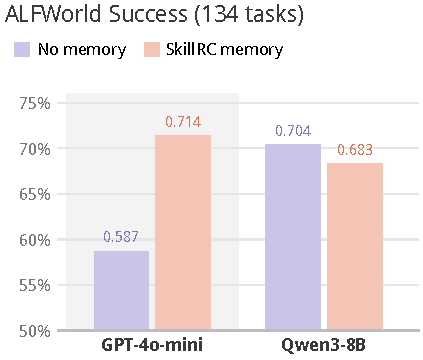
\includegraphics[width=\textwidth]{figures/fig_success.pdf}\\[-2pt]
{\small (a) Success without and with memory}
\end{minipage}\hfill
\begin{minipage}[b]{0.585\textwidth}
\centering
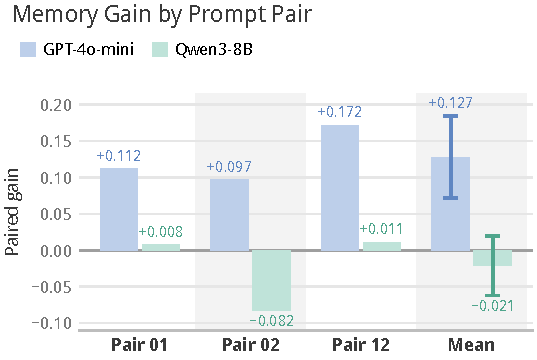
\includegraphics[width=\textwidth]{figures/fig_pairs.pdf}\\[-2pt]
{\small (b) Paired gain per demonstration pair}
\end{minipage}
\vspace{2pt}
\caption{ALFWorld results for the 645-token experience memory. (a) Equal-pair
success: the memory raises \gptm from $0.587$ to $0.714$ but not \qwenm. (b) Paired
gain on each demonstration pair and the equal-pair mean with its 95\%
task-bootstrap interval. \gptm gains on every pair; the transport gap
$\Delta_{E\times M}=-0.148$ excludes zero.}
\label{fig:success}
\vspace{-8pt}
\end{figure}

Figure~\ref{fig:success}a compares the no-memory harness with the experience-memory
harness under both executor stacks. For \gptm, the memory raises success from
$0.587$ to $0.714$, a paired gain of $+0.127$ (\ci{+0.072}{+0.184}). The gain is
present on every demonstration pair ($+0.112$, $+0.097$, and $+0.172$ on pairs 01,
02, and 12), so it is not produced by one favorable prompt. It is also obtained
with the smallest payload we test: the compact insights realize 645 memory tokens,
whereas raw trajectories and Markdown procedures realize 1{,}779--1{,}989 tokens
under the same budget and none of them exceeds this gain (RQ5).

The improvement is therefore real within the stack where the memory was built:
the same frozen executor, the same scaffold, and the same tasks become more
successful when 33 distilled rules are placed in context. This is the effect that
experience-driven harnesses are designed to produce, and it is the reference
point for the questions that follow.

\noindent\rqtag{RQ2}\hspace{0.45em}\textbf{Does the improvement transfer across executor stacks?}\par\nopagebreak



It does not. Under \qwenm, the same memory moves success from $0.704$ to $0.683$,
a change of $-0.021$ (\ci{-0.062}{+0.020}), and the pairwise effects are $+0.008$,
$-0.082$, and $+0.011$ (Figure~\ref{fig:success}b). The transport gap is
$\Delta_{E\times M}=-0.148$ (\ci{-0.218}{-0.080}). The focal contrast was
designated after a seed-axis audit showed that two nominal seeds selected the same
demonstration pair (Appendix~\ref{app:seedaxis}); using only the two originally
observed pairs gives a gap of $-0.170$ (\ci{-0.252}{-0.088}).

\begin{observationbox}
The improvement does not transfer, and the gap is not explained by one prompt
pair. The second stack starts from higher no-memory success ($70.4\%$ against
$58.7\%$), leaving less headroom, and RQ3 shows that it also responds to the added
block differently. The interval identifies moderation of the whole
payload by the stack; it does not identify which stack component, whether weights,
tokenizer, template, or runtime, is responsible.
\end{observationbox}

\noindent\rqtag{RQ3}\hspace{0.45em}\textbf{Is the improvement driven by experience content?}\par\nopagebreak

\begin{figure}[t]
\centering
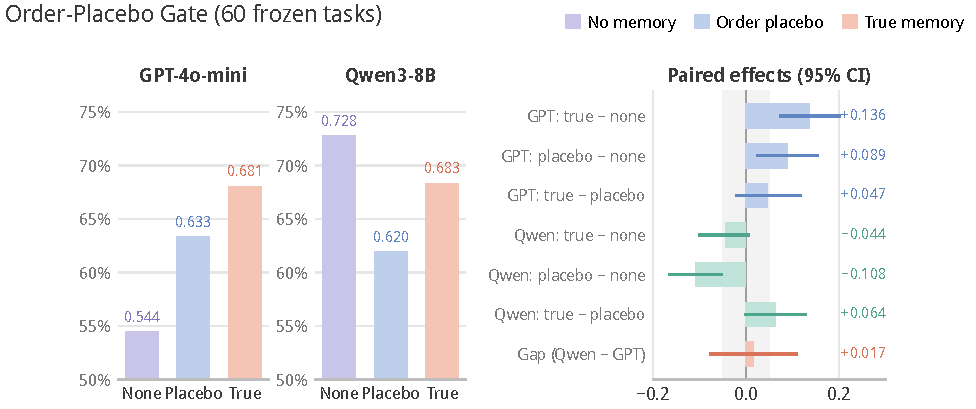
\includegraphics[width=\textwidth]{figures/fig_placebo.pdf}
\vspace{-14pt}
\caption{Pre-registered order-placebo gate on 60 frozen tasks. Left: equal-pair
success under no memory, the order placebo, and the true memory; placebo success
equals no-memory success plus the reported placebo effect. Right: paired effects
with 95\% stratified task-bootstrap intervals; the grey band is the frozen
equivalence region $[-0.05,+0.05]$.}
\label{fig:placebo}
\vspace{-8pt}
\end{figure}

Only partly. On the 60-task gate the true memory reproduces the original
direction: \gptm rises from $0.544$ to $0.681$ ($+0.136$, \ci{+0.075}{+0.200}) and
\qwenm falls from $0.728$ to $0.683$ ($-0.044$, \ci{-0.100}{+0.006}). The placebo,
which carries the same items in the same order at the same footprint but no
coherent text, already moves the stacks apart: $+0.089$ for \gptm
(\ci{+0.025}{+0.153}) and $-0.108$ for \qwenm (\ci{-0.164}{-0.053};
Figure~\ref{fig:placebo}). Coherent content then adds $S_G=+0.047$ for \gptm
(\ci{-0.019}{+0.117}; 21/16/23 task wins, losses, and ties) and $S_Q=+0.064$ for
\qwenm (\ci{0.000}{+0.128}; 18/11/31). The gap in this increment is
$\Delta_{E\times S}=+0.017$ (\ci{-0.075}{+0.108}).

\begin{observationbox}
Under the frozen rule the content mechanism is \emph{inconclusive}: coherent text
may add a modest increment for both stacks, but the executor reversal of RQ2
cannot be attributed to differential use of experience content. In point
estimates, the placebo alone opens a stack gap of $-0.197$, as large as the true
memory's $-0.181$ on the same tasks. Most of the transport gap is a difference in
how the two stacks respond to an added block of task-tagged action vocabulary.
\end{observationbox}

\noindent\rqtag{RQ4}\hspace{0.45em}\textbf{Where does transfer succeed or fail across tasks?}\par\nopagebreak

\begin{figure}[t]
\centering
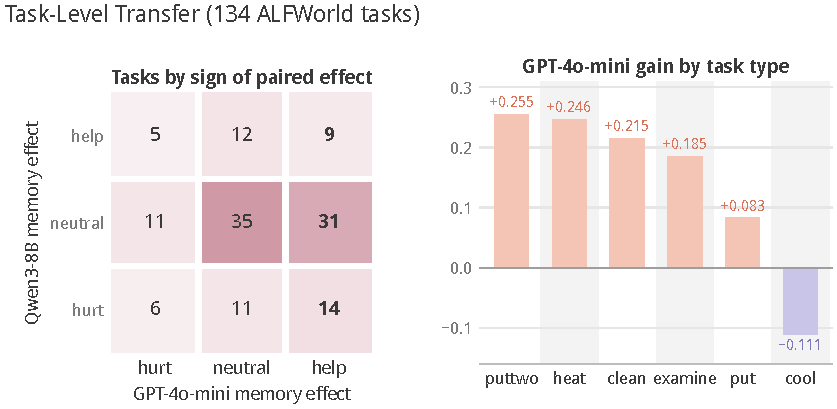
\includegraphics[width=\textwidth]{figures/fig_transport.pdf}
\vspace{-14pt}
\caption{Task-level transfer. Left: the 134 ALFWorld tasks by the sign of their
equal-pair memory effect under each stack. Right: \gptm gain by task type in the
nominal-seed matrix.}
\label{fig:transport}
\vspace{-8pt}
\end{figure}

Transfer is heterogeneous (Figure~\ref{fig:transport}). Only 9 tasks improve under
both stacks and 6 decline under both. Forty-five improve under \gptm but are
neutral (31) or harmed (14) under \qwenm, and 17 show the converse. Thirteen of the
14 tasks that help \gptm and hurt \qwenm have \qwenm no-memory success of at least
two thirds, against a mean of $0.407$ among tasks that help both, which is
compatible with a ceiling-plus-interference account but does not establish it.
Task types differ as well: \gptm gains range from $+0.255$ on \texttt{puttwo} and
$+0.246$ on \texttt{heat} to $-0.111$ on \texttt{cool}, and the types with the
weakest \gptm baseline gain the most. Cross-fitted difficulty, which classifies
each observation using only the other two no-memory observations of the same task,
shows \gptm gains declining from $+0.261$ on hard tasks to $+0.157$ on mixed and
$+0.048$ on easy ones, while \qwenm shows no monotone pattern
(Appendix~\ref{app:taxonomy}; Appendix~\ref{app:cases} walks through one case per task type).

\noindent\rqtag{RQ5}\hspace{0.45em}\textbf{Is more experience context better, and does the pattern hold elsewhere?}\par\nopagebreak

\begin{table}[t]
\centering
\caption{Realized memory tokens and paired success gains for each memory
representation and presentation in the exploratory matrix (nominal seeds
0--2; intervals in Appendix~\ref{app:matrix}). Raw trajectories were not run under
\qwenm. The highlighted row is the focal \method memory.}
\label{tab:cost}
\footnotesize
\setlength{\tabcolsep}{6pt}
\renewcommand{\arraystretch}{1.14}
\arrayrulecolor{tableline}
\begin{tabular}{@{}llrrrr@{}}
\toprule
\rowcolor{tableheadbg}
\tablehead{Representation} & \tablehead{Presentation} & \tablehead{Memory tokens} &
\tablehead{\texttt{GPT-4o-mini} $\Delta$} & \tablehead{\texttt{Qwen3-8B} $\Delta$} & \tablehead{Gap} \\
\midrule
\rowcolor{tableaccentbg}
\textbf{\textcolor{narrareddeep}{Compact insights}} & \textbf{\textcolor{narrareddeep}{BM25}}
  & \textbf{\textcolor{narrareddeep}{645}} & \textbf{\textcolor{narrareddeep}{$+0.147$}}
  & \textbf{\textcolor{narrareddeep}{$-0.020$}} & \textbf{\textcolor{narrareddeep}{$-0.167$}} \\
Compact insights & dense & 645 & $+0.070$ & $-0.005$ & $-0.075$ \\
\rowcolor{tablestripebg}
Raw trajectories & BM25 & 1{,}780 & $+0.072$ & -- & -- \\
Raw trajectories & dense & 1{,}779 & $+0.105$ & -- & -- \\
\rowcolor{tablestripebg}
Markdown procedures & BM25 & 1{,}989 & $+0.047$ & $-0.077$ & $-0.124$ \\
Markdown procedures & dense & 1{,}970 & $+0.097$ & $-0.062$ & $-0.159$ \\
\bottomrule
\end{tabular}
\arrayrulecolor{black}
\vspace{-10pt}
\end{table}

More context does not buy more utility (Table~\ref{tab:cost}). The strongest
\gptm condition injects the fewest tokens, while trajectory and procedural
memories, roughly three times larger under the same nominal budget, never exceed
the compact BM25 gain, and Markdown procedures harm \qwenm under both presentations ($-0.077$
and $-0.062$, both intervals below zero). Because the 33 insights always fit,
BM25 versus dense ranking changes only their order, yet order alone moves the
\gptm gain from $+0.147$ to $+0.070$; the executor-by-presentation interaction is
$-0.092$ (\ci{-0.162}{-0.020}). In a balanced 12-task matched-footprint pilot, no
memory and all three compressed memories each solve 5/12 tasks, but different
ones, which points to task reallocation rather than equal-footprint superiority. The memory is also cheap for the stack it helps: \gptm episodes become shorter
(18.1 against 20.3 steps), so the 645-token block raises total prompt tokens by 16.1\%
and API cost by 9.6\%, most of it cached (Appendix~\ref{app:per_type}).

\begin{figure}[t]
\centering
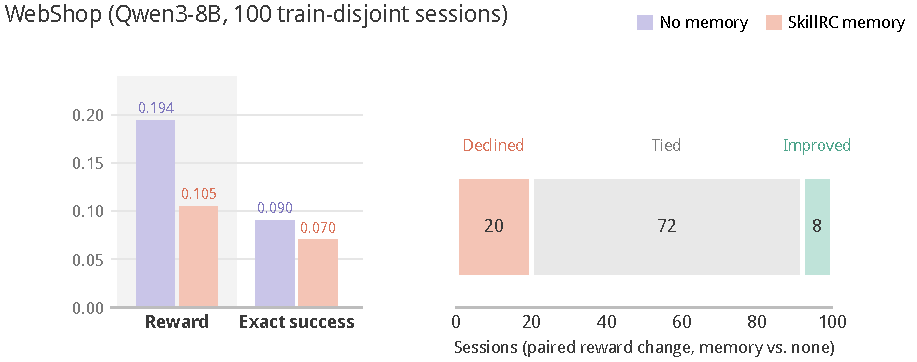
\includegraphics[width=\textwidth]{figures/fig_webshop.pdf}
\vspace{-14pt}
\caption{Train-disjoint WebShop comparison with local \qwenm. Left: mean reward and
exact purchase success without and with a ten-rule experience memory. Right: sign
of the paired reward change over 100 sessions.}
\label{fig:webshop}
\vspace{-8pt}
\end{figure}

In WebShop, a 20-task gate first confirmed that \qwenm executes validly (100\%
valid action syntax, search on 20/20 tasks, 13 purchase attempts, mean reward
$0.288$). We distilled ten ExpeL-style rules from the six positive-reward
trajectories of train sessions 500--519 and compared no memory with this pool on
disjoint sessions 0--99. Reward falls from $0.194$ to $0.105$ (paired $-0.090$,
\ci{-0.165}{-0.016}), with 8 improvements, 20 declines, and 72 ties, and exact
success moves from $0.09$ to $0.07$ ($-0.020$, \ci{-0.090}{+0.050};
Figure~\ref{fig:webshop}).

\begin{observationbox}
Experience memory can reduce performance outright. The WebShop pool was distilled
from only six positive trajectories and was read by the stack that also showed no
ALFWorld gain; it has twice as many task losses as wins. This check uses one
executor and no placebo, so it is a bounded negative-transfer replication rather
than an estimate of executor moderation in WebShop.
\end{observationbox}

\section{Conclusion}
\label{sec:conclusion}

\vspace{-5pt}

We presented \method, a reality check for experience memory in agent harnesses. It
varies only the executor stack and the memory's content, representation,
presentation, and footprint, audits what reaches the model, and evaluates the memory
through paired transport gaps and a pre-registered, payload-matched placebo. On ALFWorld, the memory improves one
executor stack with the most compact representation, but the improvement does not
transfer, and a placebo that keeps the items, order, and footprint reproduces the
reversal. Experience-driven harnesses can therefore report a genuine gain whose
source is the stack's response to added context rather than the experience
content. Future work should manipulate stack components one at a time, extend the
placebo to regimes where retrieval changes membership, and apply the same audit to
harnesses that learn their memories online.

\bibliographystyle{plainnat}
\bibliography{references}

\appendix

\section*{Appendix Contents}
\label{app:contents}
\begin{tcolorbox}[
  enhanced,
  colback=tableheadbg,
  colframe=tableaccentrule,
  boxrule=0.5pt,
  arc=2pt,
  left=7pt,
  right=7pt,
  top=6pt,
  bottom=6pt
]
\small
\renewcommand{\arraystretch}{1.18}
\begin{tabular*}{\linewidth}{@{\extracolsep{\fill}}C{0.08\linewidth}L{0.70\linewidth}r@{}}
\textbf{\textcolor{narrareddeep}{\ref{sec:limitations}}}
  & \hyperref[sec:limitations]{Limitations}
  & \textcolor{remarkgray}{p.~\pageref{sec:limitations}} \\
\textbf{\textcolor{narrareddeep}{\ref{app:implementation_details}}}
  & \hyperref[app:implementation_details]{Implementation details}
  & \textcolor{remarkgray}{p.~\pageref{app:implementation_details}} \\
\textbf{\textcolor{narrareddeep}{\ref{app:prompts}}}
  & \hyperref[app:prompts]{Prompt settings}
  & \textcolor{remarkgray}{p.~\pageref{app:prompts}} \\
\textbf{\textcolor{narrareddeep}{\ref{app:memory}}}
  & \hyperref[app:memory]{Experience memory contents}
  & \textcolor{remarkgray}{p.~\pageref{app:memory}} \\
\textbf{\textcolor{narrareddeep}{\ref{app:experimental_details}}}
  & \hyperref[app:experimental_details]{Experimental details}
  & \textcolor{remarkgray}{p.~\pageref{app:experimental_details}} \\
\textbf{\textcolor{narrareddeep}{\ref{app:per_type}}}
  & \hyperref[app:per_type]{Per-task-type results and cost}
  & \textcolor{remarkgray}{p.~\pageref{app:per_type}} \\
\textbf{\textcolor{narrareddeep}{\ref{app:models}}}
  & \hyperref[app:models]{Models used}
  & \textcolor{remarkgray}{p.~\pageref{app:models}} \\
\textbf{\textcolor{narrareddeep}{\ref{app:comparison_scope}}}
  & \hyperref[app:comparison_scope]{Comparison scope}
  & \textcolor{remarkgray}{p.~\pageref{app:comparison_scope}} \\
\textbf{\textcolor{narrareddeep}{\ref{sec:related}}}
  & \hyperref[sec:related]{Related work}
  & \textcolor{remarkgray}{p.~\pageref{sec:related}} \\
\textbf{\textcolor{narrareddeep}{\ref{app:matrix}}}
  & \hyperref[app:matrix]{Representation matrix and executor interactions}
  & \textcolor{remarkgray}{p.~\pageref{app:matrix}} \\
\textbf{\textcolor{narrareddeep}{\ref{app:taxonomy}}}
  & \hyperref[app:taxonomy]{Task-level transfer diagnostic}
  & \textcolor{remarkgray}{p.~\pageref{app:taxonomy}} \\
\textbf{\textcolor{narrareddeep}{\ref{app:cases}}}
  & \hyperref[app:cases]{Case studies}
  & \textcolor{remarkgray}{p.~\pageref{app:cases}} \\
\textbf{\textcolor{narrareddeep}{\ref{app:seedaxis}}}
  & \hyperref[app:seedaxis]{Seed-axis audit}
  & \textcolor{remarkgray}{p.~\pageref{app:seedaxis}} \\
\textbf{\textcolor{narrareddeep}{\ref{app:placebo}}}
  & \hyperref[app:placebo]{Order-placebo construction}
  & \textcolor{remarkgray}{p.~\pageref{app:placebo}}
\end{tabular*}
\end{tcolorbox}
\vspace{-6pt}

\section{Limitations}
\label{sec:limitations}

This study has several limitations. First, the executor contrast bundles model
weights, tokenizers, chat templates, serving systems, and generation
repeatability; it establishes stack-level moderation, not a model-weight
mechanism. Second, the focal contrast was designated after a seed-axis audit, and
the representation matrix, task-type, difficulty, and taxonomy analyses are
exploratory and not adjusted for multiplicity. Third, the study covers two
executor stacks, one focal 33-item pool, and ALFWorld; it is not a population
estimate over models or experience artifacts, and the representation reproductions
omit the optimizers and curators of ExpeL and SkillOS. Fourth, the order placebo
isolates coherent local order imperfectly: shuffled text may distract differently
from coherent text, and retained words keep bag-of-words cues; the 60-task gate is
also lower powered than the 134-task focal contrast and targets an equal-task-type
effect. Fifth, the WebShop check uses one local executor, one train-distilled pool,
the small environment, and one execution per condition. Finally, the hosted GPT
alias is mutable and temperature-zero hosted generations are not perfectly
deterministic, and the public release contains the harness, configurations, pools,
and analysis code but not per-episode logs, so the figures are drawn from the
frozen summary statistics.

\section{Implementation Details}
\label{app:implementation_details}

This appendix describes how the abstract components of
Section~\ref{sec:method}, namely the harness configuration, the memory payload,
the audit, and the placebo, are realized in our reference implementation. None of
these choices alters the estimands; they specify how the abstract objects are
instantiated in the experiments of Section~\ref{sec:experiments}.

\paragraph{Harness representation.}
A configuration $H=(E,M,d)$ is materialized as one YAML file: the executor endpoint
($E$), the memory kind and pool path ($c$, $r$), the retriever and an optional
index-aligned ranking reference ($p$), the token budget $B$ and item cap $K$, and the
demonstration file and seed ($d$). The remaining keys, namely decoding parameters,
prompt style, admissible-action injection, step limit, and environment, take the
same values in every configuration of a comparison. Unknown keys are rejected at
load time so that a configuration cannot silently omit a setting.

\paragraph{Initialization.}
Every comparison starts from the no-memory configuration ($c=$ none), whose prompt
contains only the task scaffold and two demonstrations. A memory condition adds one
block after the scaffold and changes nothing else; the executor client, decoding,
ReAct loop, and action parsing are shared code paths.

\paragraph{Memory construction.}
The ALFWorld pools are distilled with \gptm from successful trajectories on the
seen validation split, using at most six trajectories per task type: 33
natural-language insights (ExpeL-style), raw successful trajectories, and one
Markdown procedure per successful trajectory (SkillOS-style). The WebShop pool
holds ten rules distilled by local \qwenm.

\paragraph{Presentation and budget fill.}
All pool memories share one fill path. Items are ranked, appended greedily until the
next item would exceed $B$ (or $K$ items when no budget is set), and the
concatenation is truncated to $B$ tokens keeping its beginning. Only the ranking
differs across presentations: whitespace-tokenized BM25, dense cosine similarity
over \texttt{text-embedding-3-small} vectors, or lexical overlap. When a ranking
reference is supplied, BM25 is fit on the reference pool and the payload items are
returned at the reference indices, which is how the placebo inherits the true
memory's order exactly.

\paragraph{Payload accounting.}
Realized memory tokens are counted with the executor-appropriate tokenizer
(\texttt{tiktoken} for \gptm, the native tokenizer for the \qwenm audit) and logged
per episode, so footprint is reported as realized rather than nominal. The executor
client also records prompt, completion, and cached tokens for every call and
forwards \texttt{chat\_template\_kwargs} to disable Qwen3 thinking.

\section{Prompt Settings}
\label{app:prompts}

This appendix reproduces every prompt used in the study, verbatim from the
released code. All prompts are shared by every memory condition; a memory
condition only appends the block headed \texttt{\# Retrieved experience / skills},
whose items and order are set by the memory's representation and presentation.
Angle brackets mark slots
that are filled at run time.

\paragraph{ALFWorld agent (ReAct, both executors).}
Each call sends two messages. The system message holds the instruction, the two
demonstrations selected for the task type, and the memory block; it is constant
within an episode, which makes it cacheable. The user message holds the growing
transcript, the admissible actions, and a trailing prompt character. The example
below uses the real initial observation of task~0.

\begin{promptbox}{System message (ALFWorld)}
Interact with a household to solve a task. Output only the next line: either an action, or a line beginning with 'think:' to reason (a 'think:' line is not an environment action). Here are two examples.

<ReAct demonstration react_<type>_<i>>

<ReAct demonstration react_<type>_<j>>

Here is the task.

# Retrieved experience / skills
<33 insights in BM25 order, one per paragraph, 645 tokens in total>
\end{promptbox}

\begin{promptbox}{User message (ALFWorld, first turn of task 0)}
-= Welcome to TextWorld, ALFRED! =-

You are in the middle of a room. Looking quickly around you, you see a bed 1, a desk 2, a desk 1, a drawer 6, a drawer 5, a drawer 4, a drawer 3, a drawer 2, a drawer 1, a garbagecan 1, a laundryhamper 1, a safe 1, a shelf 6, a shelf 5, a shelf 4, a shelf 3, a shelf 2, and a shelf 1.

Your task is to: put a mug in desk.
Valid actions right now: <admissible commands, separated by '; '>
>
\end{promptbox}

\noindent
The executor's reply is parsed as its first non-empty line with any leading
\texttt{>} removed. A line beginning with \texttt{think:} is appended to the
transcript and answered with \texttt{OK.} without consuming an environment step;
any other line is executed. Because this ALFWorld version uses the verb
\texttt{move X to Y}, a reply of the form \texttt{put X in/on Y} is rewritten to
that grammar for every condition. Each subsequent user message is the full
transcript (\texttt{> action} followed by the observation) plus the current
admissible actions. An episode ends on success, after 30 environment steps, or
after 60 executor calls.

\paragraph{WebShop agent (Thought/Action).}
WebShop uses the generic Thought/Action scaffold with two worked examples and the
same memory header. The reply is parsed by its last \texttt{Action:} line.

\begin{promptbox}{System message (WebShop)}
You are an agent solving an interactive text task using the ReAct framework.
At each step: first write one short line starting with 'Thought:' with your reasoning, then output exactly one line starting with 'Action:' containing a single admissible action. Output nothing after the Action line.

# Examples
Task: Find a red cotton shirt under $30.
Thought: I should search using the requested attributes.
Action: search[red cotton shirt]
Observation: Search results include product ids.
Thought: I should inspect the most relevant product.
Action: click[b012example]
Observation: Product page with options and Buy Now.
Thought: I should select the requested option before buying.
Action: click[red]
Observation: Red is selected.
Thought: The item matches, so I should purchase it.
Action: click[buy now]

<second example: a 32-ounce insulated water bottle, same format>

# Retrieved experience / skills
<WebShop rules in BM25 order, at most 1,024 tokens>
\end{promptbox}

\begin{promptbox}{User message (WebShop)}
<WebShop observation, including the instruction>

# Valid actions right now
<admissible actions, separated by '; '>

# Interaction so far
<previous Action/Observation pairs, or "(none yet)">

What is your next Thought and Action?
\end{promptbox}

\paragraph{Memory distillation (building the pools).}
The pools are built offline from training-only trajectories with the following
prompts. Compact insights use the first prompt once per task type with at most six
successful trajectories; Markdown procedures use the second prompt once per
successful trajectory; the WebShop pool uses the third prompt on train sessions
500--519.

\begin{promptbox}{Insight distillation (ExpeL-style, ALFWorld)}
Below are successful agent trajectories for ALFWorld '<task_type>' tasks.
Extract 3 to 6 concise, GENERAL insights (rules/heuristics) that help solve this task type. Each insight: one imperative line, no specific object numbers or room layouts. Output ONLY a bullet list, each line starting with '- '.

Trajectories:
<up to six successful trajectories of this type, separated by '---'>
\end{promptbox}

\begin{promptbox}{Procedure distillation (SkillOS-style Markdown, ALFWorld)}
Below is a successful agent trajectory in ALFWorld.
Distill it into ONE reusable skill in Markdown with exactly:
'## Skill: <short name>', a 'When to use:' line, and a 'Steps:' numbered list (generalized — describe the procedure, not the specific object numbers). Keep it under 110 words.

Trajectory:
<one successful trajectory>
\end{promptbox}

\begin{promptbox}{Rule distillation (WebShop)}
You are distilling reusable procedural insights for the WebShop text environment.
The examples below come only from training sessions disjoint from evaluation.
Extract 6 to 10 concise general rules that improve product search, attribute checking,
option selection, and purchase decisions. Do not mention product IDs, session IDs, or
specific products. Output only bullet lines beginning with '- '.

Training experiences:
<positive-reward trajectories from train sessions 500-519>
\end{promptbox}

\paragraph{Decoding.}
All executor calls use temperature 0 and at most 256 completion tokens. \qwenm is
served by vLLM with \texttt{chat\_template\_kwargs = \{"enable\_thinking": false\}};
\gptm uses the provider defaults otherwise. Distillation calls use the same
decoding with at most 512 completion tokens.

\section{Experience Memory Contents}
\label{app:memory}

Table~\ref{tab:pool} lists the complete focal experience memory, the 33 ExpeL-style
insights distilled with the prompt above. Every item carries a task-type tag, and
all 33 items (645 tokens) are injected on every task, so BM25 decides only their
order. The order placebo keeps each item's tag, index, and word count; the first
\texttt{[clean]} item, for example, becomes \texttt{[clean] the the item cleaning its
starting requirements x and target Identify before}
(Appendix~\ref{app:placebo}).

\begin{table}[t]
\centering
\caption{The 33-item experience memory used in every ALFWorld memory condition, in
pool order. Counts per type: \texttt{clean} 5, \texttt{cool} 6, \texttt{examine} 6,
\texttt{heat} 5, \texttt{put} 6, \texttt{puttwo} 5.}
\label{tab:pool}
\scriptsize
\setlength{\tabcolsep}{5pt}
\renewcommand{\arraystretch}{1.08}
\arrayrulecolor{tableline}
\begin{tabular}{@{}r l L{0.80\textwidth}@{}}
\toprule
\rowcolor{tableheadbg}
\tablehead{\#} & \tablehead{Type} & \tablehead{Insight} \\
\midrule
\rowcolor{tablestripebg}
0 & \texttt{clean} & Identify the target item and its cleaning requirements before starting the task. \\
1 & \texttt{clean} & Prioritize checking locations where the target item is likely to be found, such as countertops, cabinets, and drawers. \\
\rowcolor{tablestripebg}
2 & \texttt{clean} & Always clean the item using the designated cleaning area before placing it in the final location. \\
3 & \texttt{clean} & Confirm the cleanliness of the item if necessary before moving it to the final destination. \\
\rowcolor{tablestripebg}
4 & \texttt{clean} & Ensure to follow the sequence of actions: find, clean, and then place the item correctly. \\
5 & \texttt{cool} & Start by identifying likely locations for the target item based on its type. \\
\rowcolor{tablestripebg}
6 & \texttt{cool} & Always check the fridge first for items that need to be cooled. \\
7 & \texttt{cool} & If the desired item is not found, systematically explore other potential locations. \\
\rowcolor{tablestripebg}
8 & \texttt{cool} & After obtaining the item, ensure to cool it before proceeding to the final placement. \\
9 & \texttt{cool} & Confirm the availability of the final destination before moving the item there. \\
\rowcolor{tablestripebg}
10 & \texttt{cool} & Maintain a clear sequence of actions: find, cool, and place the item. \\
11 & \texttt{examine} & Identify the required items and prioritize searching in likely locations based on their common placements. \\
\rowcolor{tablestripebg}
12 & \texttt{examine} & Check multiple potential locations systematically if the first search does not yield results. \\
13 & \texttt{examine} & Use the most probable locations for the second required item after obtaining the first. \\
\rowcolor{tablestripebg}
14 & \texttt{examine} & Always confirm the presence of an item before attempting to use it. \\
15 & \texttt{examine} & If an item is not found in one location, move to the next logical location without skipping options. \\
\rowcolor{tablestripebg}
16 & \texttt{examine} & Ensure to use the item in the correct context to achieve the task's goal. \\
17 & \texttt{heat} & Identify the target item and its required state before proceeding with the task. \\
\rowcolor{tablestripebg}
18 & \texttt{heat} & Prioritize checking locations where the target item is likely to be found. \\
19 & \texttt{heat} & Use appropriate appliances or tools to modify the item as needed before completing the task. \\
\rowcolor{tablestripebg}
20 & \texttt{heat} & Ensure to open or interact with containers before placing or retrieving items. \\
21 & \texttt{heat} & Maintain a clear sequence of actions to avoid unnecessary backtracking. \\
\rowcolor{tablestripebg}
22 & \texttt{put} & Start by checking locations where the target object is likely to be found, such as tables, countertops, or drawers. \\
23 & \texttt{put} & If the initial location does not contain the target object, systematically explore other nearby locations. \\
\rowcolor{tablestripebg}
24 & \texttt{put} & Always check closed containers (drawers, cabinets) before assuming the object is not present. \\
25 & \texttt{put} & Once the target object is found, plan the route to the designated location for placing it. \\
\rowcolor{tablestripebg}
26 & \texttt{put} & Ensure to confirm the target object is in your possession before attempting to place it. \\
27 & \texttt{put} & When placing the object, verify that the destination is clear and appropriate for the item. \\
\rowcolor{tablestripebg}
28 & \texttt{puttwo} & Start by identifying the most likely locations for the target items based on their type. \\
29 & \texttt{puttwo} & Check each location systematically, ensuring to open closed containers before searching inside. \\
\rowcolor{tablestripebg}
30 & \texttt{puttwo} & Once an item is found, immediately plan the next steps to retrieve and place it in the designated location. \\
31 & \texttt{puttwo} & If the first search does not yield results, revisit previously checked locations, as items may be present in multiple instances. \\
\rowcolor{tablestripebg}
32 & \texttt{puttwo} & Keep track of items already found and placed to avoid unnecessary repetition in searches. \\
\bottomrule
\end{tabular}
\arrayrulecolor{black}
\vspace{-8pt}
\end{table}

\section{Experimental Details}
\label{app:experimental_details}

\paragraph{Benchmarks.}
ALFWorld \citep{shridhar2021alfworld} is evaluated on its 134-task unseen split,
covering \texttt{clean}, \texttt{cool}, \texttt{examine}, \texttt{heat},
\texttt{put}, and \texttt{puttwo}, with binary success within 30 steps. WebShop
\citep{yao2022webshop} is evaluated in its small environment with 1{,}000 products
(official commit \texttt{64fa2a5c15c7}) and a 15-step limit; environment reward is
the primary outcome and exact purchase success is secondary.

\paragraph{Baselines.}
The baseline for every stack is the no-memory harness $W_0$. Exploratory memory
conditions are raw successful trajectories and SkillOS-style Markdown procedures
under the same insertion point and nominal budget; these are representation
reproductions under one harness, not reimplementations of the source systems'
optimizers or curators. For content attribution, the baseline is the
payload-matched order placebo of Section~\ref{sec:placebo}.

\paragraph{Models and protocol.}
Nominal seeds 0, 1, and 2 select demonstration pairs 02, 12, and 12; seed 5 was run
to supply pair 01 (Appendix~\ref{app:seedaxis}). The focal contrast weights pairs
01, 02, and 12 equally and averages the two executions of pair 12. The placebo gate
reuses the matching no-memory and true-memory episodes and runs only the placebo
under both stacks with $B=645$.

\paragraph{Hyperparameters and splits.}
Table~\ref{tab:hparams} lists the settings held fixed across conditions. ALFWorld
intervals resample the 134 task clusters 10{,}000 times; the placebo gate resamples
ten tasks with replacement within each task type (20{,}000 draws, seed 20260713);
WebShop uses 20{,}000 paired task-bootstrap draws, and its gate, split, primary
outcome, and stopping rule were frozen before the 100-session comparison.

\begin{table}[t]
\centering
\caption{Hyperparameters held fixed across conditions.}
\label{tab:hparams}
\footnotesize
\setlength{\tabcolsep}{8pt}
\renewcommand{\arraystretch}{1.14}
\arrayrulecolor{tableline}
\begin{tabular}{@{}ll@{}}
\toprule
\rowcolor{tableheadbg}
\tablehead{Parameter} & \tablehead{Value} \\
\midrule
\rowcolor{tablestripebg}
Temperature & 0 \\
Completion cap per turn & 256 tokens \\
\rowcolor{tablestripebg}
Demonstrations per prompt & 2 of 3 per task type \\
Step limit (ALFWorld / WebShop) & 30 / 15 \\
\rowcolor{tablestripebg}
Memory budget $B$ (ALFWorld / WebShop / placebo gate) & 2{,}048 / 1{,}024 / 645 \\
Item cap $K$ & 20 \\
\rowcolor{tablestripebg}
\qwenm max model length & 16{,}384 \\
Bootstrap draws (ALFWorld / gate / WebShop) & 10{,}000 / 20{,}000 / 20{,}000 \\
\bottomrule
\end{tabular}
\arrayrulecolor{black}
\vspace{-10pt}
\end{table}

\section{Per-Task-Type Results and Cost}
\label{app:per_type}

Tables~\ref{tab:pertype} and~\ref{tab:costfull} report the per-type success and the
full token and cost accounting of the four runs behind the focal comparison in the
nominal-seed matrix (402 episodes each: 134 tasks $\times$ seeds 0--2). The run
summaries are released with the code.

\begin{table}[t]
\centering
\caption{ALFWorld success by task type without memory, with the 645-token
experience memory (compact insights + BM25), and the difference, for both executor
stacks (nominal seeds 0--2). \textcolor{liftpositive}{Green}: gain;
\textcolor{liftnegative}{red}: loss.}
\label{tab:pertype}
\footnotesize
\setlength{\tabcolsep}{6pt}
\renewcommand{\arraystretch}{1.12}
\arrayrulecolor{tableline}
\begin{tabular}{@{}lr ccc ccc@{}}
\toprule
\rowcolor{tableheadbg}
& & \multicolumn{3}{c}{\tablehead{\texttt{GPT-4o-mini}}} & \multicolumn{3}{c}{\tablehead{\texttt{Qwen3-8B}}} \\
\rowcolor{tableheadbg}
\tablehead{Task type} & \tablehead{Episodes} & \tablehead{None} & \tablehead{Memory} & \tablehead{$\Delta$} & \tablehead{None} & \tablehead{Memory} & \tablehead{$\Delta$} \\
\midrule
\rowcolor{tablestripebg}
\texttt{clean} & 93 & 0.452 & 0.667 & \textcolor{liftpositive}{$+0.215$} & 0.656 & 0.613 & \textcolor{liftnegative}{$-0.043$} \\
\texttt{cool} & 63 & 0.857 & 0.746 & \textcolor{liftnegative}{$-0.111$} & 0.857 & 0.857 & $0.000$ \\
\rowcolor{tablestripebg}
\texttt{examine} & 54 & 0.648 & 0.833 & \textcolor{liftpositive}{$+0.185$} & 0.611 & 0.574 & \textcolor{liftnegative}{$-0.037$} \\
\texttt{heat} & 69 & 0.130 & 0.377 & \textcolor{liftpositive}{$+0.246$} & 0.739 & 0.754 & \textcolor{liftpositive}{$+0.014$} \\
\rowcolor{tablestripebg}
\texttt{put} & 72 & 0.833 & 0.917 & \textcolor{liftpositive}{$+0.083$} & 0.736 & 0.694 & \textcolor{liftnegative}{$-0.042$} \\
\texttt{puttwo} & 51 & 0.333 & 0.588 & \textcolor{liftpositive}{$+0.255$} & 0.431 & 0.431 & $0.000$ \\
\midrule
\rowcolor{tableaccentbg}
\textbf{All} & 402 & 0.540 & 0.687 & \textcolor{liftpositive}{$+0.147$} & 0.682 & 0.662 & \textcolor{liftnegative}{$-0.020$} \\
\bottomrule
\end{tabular}
\arrayrulecolor{black}
\vspace{-8pt}
\end{table}

\begin{table}[t]
\centering
\caption{Token and cost accounting for the same four runs (402 episodes each).
Token counts are in millions and summed over all calls. \qwenm is served locally,
so its dollar cost is zero and the runtime did not report cached tokens.}
\label{tab:costfull}
\footnotesize
\setlength{\tabcolsep}{5pt}
\renewcommand{\arraystretch}{1.14}
\arrayrulecolor{tableline}
\begin{tabular}{@{}llrrrrrr@{}}
\toprule
\rowcolor{tableheadbg}
\tablehead{Executor} & \tablehead{Memory} & \tablehead{Calls} & \tablehead{Steps/ep.} & \tablehead{Prompt (M)} & \tablehead{Cached (M)} & \tablehead{Output (M)} & \tablehead{Cost (\$)} \\
\midrule
\logo{openai}~\texttt{GPT-4o-mini} & none & 10{,}059 & 20.3 & 22.63 & 17.90 & 0.163 & 2.15 \\
\rowcolor{tableaccentbg}
\logo{openai}~\texttt{GPT-4o-mini} & 645 tokens & 9{,}115 & 18.1 & 26.26 & 22.31 & 0.151 & 2.36 \\
\logo{qwen-color}~\texttt{Qwen3-8B} & none & 12{,}380 & 11.1 & 32.43 & -- & 0.506 & 0.00 \\
\rowcolor{tableaccentbg}
\logo{qwen-color}~\texttt{Qwen3-8B} & 645 tokens & 12{,}262 & 10.3 & 40.68 & -- & 0.491 & 0.00 \\
\bottomrule
\end{tabular}
\arrayrulecolor{black}
\vspace{-8pt}
\end{table}

\noindent
With memory, \gptm episodes are shorter (18.1 against 20.3 steps) and make 9.4\%
fewer calls, so although every call carries 645 more tokens, total prompt tokens rise
by only 16.1\% and dollar cost by 9.6\% (\$2.36 against \$2.15 per 402 episodes).
Because the memory sits in the stable system message, 85.0\% of \gptm prompt tokens
are cached with memory against 79.1\% without it. For \qwenm the memory shortens
episodes only slightly (10.3 against 11.1 steps) and raises prompt tokens by 25.4\%.
Per type, the \gptm gains are largest where its no-memory success is lowest
(\texttt{heat}, \texttt{puttwo}, \texttt{clean}), and the only \gptm loss is on its
strongest type (\texttt{cool}); \qwenm changes by at most $0.043$ on any type.

\section{Models Used}
\label{app:models}

Table~\ref{tab:models} lists the models used in this paper. \gptm and \qwenm are
the two executor stacks of the transfer study; \gptm also distills the ALFWorld
pools, \qwenm distills the WebShop pool, and \texttt{text-embedding-3-small} is used
only for dense ranking. ``Access'' distinguishes models served only behind an API
from models whose weights are publicly released. The focal BM25 result does not
depend on the embedding service.

\begin{table}[t]
\centering
\caption{Models used in this paper. \qwenm is served with vLLM 0.24.0 from Hugging
Face snapshot \texttt{b968826d9c46} with \texttt{enable\_thinking=false}; the
\gptm alias was queried in July 2026 and has no pinned snapshot.}
\label{tab:models}
\footnotesize
\setlength{\tabcolsep}{8pt}
\renewcommand{\arraystretch}{1.20}
\arrayrulecolor{tableline}
\begin{tabular}{@{}llll@{}}
\toprule
\rowcolor{tableheadbg}
\tablehead{Model} & \tablehead{Provider} & \tablehead{Access} & \tablehead{Role} \\
\midrule
\rowcolor{tablestripebg}
\logo{openai}~\texttt{GPT-4o-mini}              & OpenAI   & Proprietary (API) & executor; ALFWorld distillation \\
\logo{qwen-color}~\texttt{Qwen3-8B}             & Alibaba  & Open weights      & executor; WebShop distillation \\
\rowcolor{tablestripebg}
\logo{openai}~\texttt{text-embedding-3-small}   & OpenAI   & Proprietary (API) & dense ranking only \\
\bottomrule
\end{tabular}
\arrayrulecolor{black}
\vspace{-15pt}
\end{table}

\section{Comparison Scope}
\label{app:comparison_scope}

\method is an evaluation harness for experience memory, not a new memory method or
harness optimizer, so it is not an empirical competitor to the systems discussed in
Appendix~\ref{sec:related}. Its comparisons are within-harness: every contrast changes
one factor of Table~\ref{tab:dimensions} on identical tasks, so the paper makes no
claim about the absolute performance of any released system. The executor contrast compares two \emph{stacks}, and we do not claim
that the difference is caused by model weights. The placebo is an experimental
control with an oracle ranking reference, not a deployable retrieval scheme, and
the representation matrix is asymmetric and exploratory rather than a ranking of
representations.

\section{Related Work}
\label{sec:related}

\subsection{Experience-Driven Harness Optimization}
\label{sec:related_harness}

Automatic improvement of LLM systems has targeted prompts
\citep{fernando2023promptbreeder}, declarative pipelines \citep{khattab2023dspy},
and agentic workflows \citep{zhang2024aflow}. Meta-Harness searches over harness
code end to end \citep{lee2026metaharness}, and \memoharness decomposes the harness
into six editable dimensions, accumulates per-case entries and global patterns in
a dual-layer experience bank, and adapts the learned harness to each test case
\citep{huang2026memoharness}. Agents that write experience into memory include
Reflexion \citep{shinn2023reflexion} and ExpeL \citep{zhao2023expel}, built on
reasoning-and-acting scaffolds such as ReAct \citep{yao2023react}. These systems
build or optimize the harness. \method instead isolates one of its components, the
experience memory, and asks whether the gain that component produces survives a
change of executor and a content control.

\subsection{Skill Libraries, Curation, and Retrieval}
\label{sec:related_skills}

SkillOpt treats a skill document as editable state accepted under held-out
validation \citep{yang2026skillopt}, SkillOS learns experience-driven skill
curation with reinforcement learning around a frozen executor
\citep{ouyang2026skillos}, and SelfEvoSkill revises skills from paired execution
audits without external outcome supervision \citep{gao2026selfevoskill}. SkillRet
benchmarks retrieval from large public skill libraries \citep{kang2026skillret},
task-decomposition-guided reranking adapts skill retrieval to execution state
\citep{chen2026reranker}, and experience reuse has been studied as continual
learning that moves into memory \citep{hu2026memory}. These systems build or select
the memory; we study whether a fixed memory transfers and why.

\subsection{Skill-Centered Evaluation}
\label{sec:related_eval}

SkillsBench finds broad average gains from curated skills with negative deltas on
some tasks \citep{li2026skillsbench}. A scalable framework evaluates agentic skills
across many agent--model configurations \citep{shaposhnikov2026framework}, and
procedural-memory management has been studied across tasks, roles, and model
backbones \citep{belikova2026procedural}. Realistic skill retrieval erodes gains
\citep{liu2026wildskills}, and SWE-Skills-Bench reports limited gains, mismatch
harms, and token overhead in software engineering \citep{han2026sweskills}. Related
frameworks unify memory, skills, and rules as points on a compression spectrum
\citep{zhang2026compression} and assess skills on utility, cost, and safety
\citep{yu2026skillaudit}. Our narrower target is identification under a fixed
artifact: a paired executor interaction combined with a payload-matched placebo.

\subsection{Prompt Sensitivity and Distraction}
\label{sec:related_prompt}

Meaning-preserving formatting changes can swing accuracy substantially
\citep{sclar2023quantifying}, and irrelevant context degrades reasoning
\citep{shi2023distracted}. The placebo result of RQ3 is an agentic instance of this
phenomenon: a lexically matched but incoherent block moves two executor stacks in
opposite directions.

\section{Representation Matrix and Executor Interactions}
\label{app:matrix}

Table~\ref{tab:matrix} reports the full exploratory matrix behind
Table~\ref{tab:cost}, with task-cluster intervals and the executor-by-memory
difference-in-differences. Three of the four executor-by-memory contrasts exclude
zero, and the presentation contrast for compact insights shows that order alone
interacts with the executor. Integrity checks on the raw episode files confirmed
402/402 episodes per run, aligned task and seed keys, zero errors, and exact
agreement between raw and stored success rates.

\begin{table}[t]
\centering
\caption{Exploratory representation matrix over nominal seeds 0--2 against each
stack's matching no-memory harness, followed by executor contrasts
(\qwenm minus \gptm). Intervals are task-clustered and unadjusted for multiplicity.
\textcolor{liftpositive}{Green}: positive effect; \textcolor{liftnegative}{red}:
negative effect.}
\label{tab:matrix}
\footnotesize
\setlength{\tabcolsep}{6pt}
\renewcommand{\arraystretch}{1.12}
\arrayrulecolor{tableline}
\begin{tabular}{@{}lllrcr@{}}
\toprule
\rowcolor{tableheadbg}
\tablehead{Stack} & \tablehead{Memory} & \tablehead{Presentation} & \tablehead{Paired $\Delta$} & \tablehead{95\% CI} & \tablehead{Tokens} \\
\midrule
\rowcolor{tablestripebg}
\texttt{GPT-4o-mini} & compact insight & BM25  & \textcolor{liftpositive}{$+0.1468$} & \ci{+0.0846}{+0.2090} & 645 \\
\texttt{GPT-4o-mini} & compact insight & dense & \textcolor{liftpositive}{$+0.0697$} & \ci{+0.0174}{+0.1244} & 645 \\
\rowcolor{tablestripebg}
\texttt{GPT-4o-mini} & raw trajectory  & BM25  & \textcolor{liftpositive}{$+0.0721$} & \ci{+0.0050}{+0.1418} & 1{,}779.7 \\
\texttt{GPT-4o-mini} & raw trajectory  & dense & \textcolor{liftpositive}{$+0.1045$} & \ci{+0.0323}{+0.1766} & 1{,}779.0 \\
\rowcolor{tablestripebg}
\texttt{GPT-4o-mini} & Markdown        & BM25  & \textcolor{liftpositive}{$+0.0473$} & \ci{-0.0025}{+0.0995} & 1{,}988.8 \\
\texttt{GPT-4o-mini} & Markdown        & dense & \textcolor{liftpositive}{$+0.0970$} & \ci{+0.0398}{+0.1542} & 1{,}969.8 \\
\rowcolor{tablestripebg}
\texttt{Qwen3-8B}    & compact insight & BM25  & \textcolor{liftnegative}{$-0.0199$} & \ci{-0.0721}{+0.0299} & 645 \\
\texttt{Qwen3-8B}    & compact insight & dense & \textcolor{liftnegative}{$-0.0050$} & \ci{-0.0597}{+0.0473} & 645 \\
\rowcolor{tablestripebg}
\texttt{Qwen3-8B}    & Markdown        & BM25  & \textcolor{liftnegative}{$-0.0771$} & \ci{-0.1343}{-0.0174} & 1{,}988.8 \\
\texttt{Qwen3-8B}    & Markdown        & dense & \textcolor{liftnegative}{$-0.0622$} & \ci{-0.1244}{-0.0025} & 1{,}969.8 \\
\midrule
\rowcolor{tableaccentbg}
\multicolumn{3}{@{}l}{Executor $\times$ insight + BM25} & \textcolor{liftnegative}{$-0.1667$} & \ci{-0.2512}{-0.0871} & \\
\multicolumn{3}{@{}l}{Executor $\times$ insight + dense} & \textcolor{liftnegative}{$-0.0746$} & \ci{-0.1567}{+0.0025} & \\
\rowcolor{tableaccentbg}
\multicolumn{3}{@{}l}{Executor $\times$ Markdown + BM25} & \textcolor{liftnegative}{$-0.1244$} & \ci{-0.1990}{-0.0498} & \\
\multicolumn{3}{@{}l}{Executor $\times$ Markdown + dense} & \textcolor{liftnegative}{$-0.1592$} & \ci{-0.2438}{-0.0746} & \\
\rowcolor{tableaccentbg}
\multicolumn{3}{@{}l}{Executor $\times$ presentation (insight, triple difference)} & \textcolor{liftnegative}{$-0.0920$} & \ci{-0.1617}{-0.0199} & \\
\bottomrule
\end{tabular}
\arrayrulecolor{black}
\vspace{-10pt}
\end{table}

\section{Task-Level Transfer Diagnostic}
\label{app:taxonomy}

A single transport gap tells us \emph{whether} the memory transfers on average; it
does not tell us \emph{which} tasks carry the gap. Table~\ref{tab:taxonomy}
classifies each of the 134 ALFWorld tasks by the sign of its equal-pair memory
effect under each stack and reports the mean effects and the mean \qwenm no-memory
success in each cell. Tasks that help \gptm and hurt \qwenm have the highest \qwenm
baseline ($0.833$), and tasks that help both have the lowest ($0.407$), the pattern
summarized in RQ4. Representative cases include task 55 (\texttt{put}; \gptm
$+0.833$, \qwenm $+0.333$) among tasks that help both, and task 133 (\texttt{heat};
\gptm $+0.833$, \qwenm $-0.333$, \qwenm baseline $1.0$) among tasks that help \gptm
and hurt \qwenm. These labels prioritize cases for trajectory review; they do not
identify mechanisms.

\begin{table}[t]
\centering
\caption{Task-level transfer diagnostic over 134 ALFWorld tasks (compact insights +
BM25, equal prompt pairs). Each row is a cell of Figure~\ref{fig:transport}.
\textcolor{liftpositive}{Green}: positive mean effect; \textcolor{liftnegative}{red}:
negative mean effect.}
\label{tab:taxonomy}
\footnotesize
\setlength{\tabcolsep}{8pt}
\renewcommand{\arraystretch}{1.10}
\arrayrulecolor{tableline}
\begin{tabular}{@{}lrrrr@{}}
\toprule
\rowcolor{tableheadbg}
\tablehead{\texttt{GPT-4o-mini} / \texttt{Qwen3-8B}} & \tablehead{Tasks} & \tablehead{GPT $\Delta$} & \tablehead{Qwen $\Delta$} & \tablehead{Qwen baseline} \\
\midrule
\rowcolor{tablestripebg}
help / help       & 9  & \textcolor{liftpositive}{$+0.444$} & \textcolor{liftpositive}{$+0.370$} & 0.407 \\
help / neutral    & 31 & \textcolor{liftpositive}{$+0.452$} & $0.000$  & 0.699 \\
\rowcolor{tablestripebg}
help / hurt       & 14 & \textcolor{liftpositive}{$+0.429$} & \textcolor{liftnegative}{$-0.357$} & 0.833 \\
neutral / help    & 12 & $0.000$  & \textcolor{liftpositive}{$+0.306$} & 0.417 \\
\rowcolor{tablestripebg}
neutral / neutral & 35 & $0.000$  & $0.000$  & 0.867 \\
neutral / hurt    & 11 & $0.000$  & \textcolor{liftnegative}{$-0.364$} & 0.636 \\
\rowcolor{tablestripebg}
hurt / help       & 5  & \textcolor{liftnegative}{$-0.267$} & \textcolor{liftpositive}{$+0.333$} & 0.333 \\
hurt / neutral    & 11 & \textcolor{liftnegative}{$-0.333$} & $0.000$  & 0.879 \\
\rowcolor{tablestripebg}
hurt / hurt       & 6  & \textcolor{liftnegative}{$-0.333$} & \textcolor{liftnegative}{$-0.417$} & 0.611 \\
\bottomrule
\end{tabular}
\arrayrulecolor{black}
\vspace{-10pt}
\end{table}

\section{Case Studies}
\label{app:cases}

This appendix walks through what each kind of task asks the agent to do, what the
experience memory offers for it, and what happened with and without the memory.
Table~\ref{tab:families} first summarizes the six ALFWorld task families. Cases~1--3
then follow three individual tasks end to end; they are the only tasks whose goal,
room, and per-episode outcomes were retained in the run logs. Cases~4--6 cover the
remaining families at the level of the family and its representative tasks, and
Case~7 covers WebShop.

\methodlabel{Sources.}
Goals and room descriptions are the environment's own text from our run logs. The
\emph{expert solution} is the walkthrough stored with each ALFWorld game file, read
directly from the benchmark data without running any model; the expert knows where
every object is, so its length is a lower bound for an agent that must search.
Episode records come from \gptm on seed 0 (demonstration pair 02). Task-level effects
are the equal-pair effects of Table~\ref{tab:taxonomy}: success is averaged over
demonstration pairs 01, 02, and 12, so $-0.333$ means that one of three pairs went
from success to failure. ``Rule rank'' is the position, among the 33 injected items,
of the first item tagged with the task's own type.

\methodlabel{What the figures show.}
ALFWorld gives the agent text only, but every ALFWorld game is generated from an ALFRED
trial recorded in the AI2-THOR 3D simulator, and the 134 unseen tasks take place in just
four rooms: a kitchen (77 tasks), a bedroom (27), a bathroom (19), and a living room
(11). To show the environment behind the text, panel (a) of each ALFWorld figure renders
the trial's room with AI2-THOR 2.1.0, the version ALFWorld uses, after restoring the
trial's object positions and states. The left image is a first-person view chosen to show
the places the expert solution visits; the right image is the room from above, with a
cone marking where the left view was taken. Labels use the names that appear in the
agent's observation, such as \texttt{shelf}, \texttt{desk}, and \texttt{garbagecan}.
Colored labels mark where the object starts (orange), the appliance applied to it
(purple), and the destination (green), and the arrow on the map follows the expert's
route. Each goal exists as three trials in the same room that differ in where objects are
placed. For Cases~1--3 we render a trial whose goal text matches the run log; for
Cases~4--6, whose goals were not retained, we render an example task of the family drawn
from the same 134 unseen tasks. Rendering runs no model. The WebShop figure shows
screenshots of the official WebShop web application serving the benchmark's
1{,}000-product catalogue. Its instruction is the one recorded for evaluation session~0;
the search and clicks are ours, chosen to show a complete purchase, and the result ranking
comes from a BM25 stand-in for the benchmark's Lucene index.

\begin{table}[t]
\centering
\caption{The six ALFWorld task families of the 134 unseen tasks. The expert procedure
is the most common walkthrough pattern; expert steps are the mean and range of the
benchmark walkthrough lengths. Success rates are from Table~\ref{tab:pertype}.}
\label{tab:families}
\footnotesize
\setlength{\tabcolsep}{4pt}
\renewcommand{\arraystretch}{1.18}
\arrayrulecolor{tableline}
\begin{tabular}{@{}l r L{0.36\textwidth} c c c@{}}
\toprule
\rowcolor{tableheadbg}
\tablehead{Family} & \tablehead{Tasks} & \tablehead{What the goal requires (expert procedure)} & \tablehead{Expert steps} & \tablehead{\texttt{GPT-4o-mini}} & \tablehead{\texttt{Qwen3-8B}} \\
\midrule
\rowcolor{tablestripebg}
\texttt{put} & 24 & find an object, take it, go to the target receptacle, place it & 4.6 (4--6) & $0.833\rightarrow0.917$ & $0.736\rightarrow0.694$ \\
\texttt{clean} & 31 & find, take, go to the sink basin, \emph{clean}, go to the target, place & 6.3 (4--7) & $0.452\rightarrow0.667$ & $0.656\rightarrow0.613$ \\
\rowcolor{tablestripebg}
\texttt{heat} & 23 & find, take, go to the microwave, \emph{heat}, go to the target, place & 6.0 (4--7) & $0.130\rightarrow0.377$ & $0.739\rightarrow0.754$ \\
\texttt{cool} & 21 & find, take, go to the fridge, \emph{cool}, go to the target, place & 6.1 (4--7) & $0.857\rightarrow0.746$ & $0.857\rightarrow0.857$ \\
\rowcolor{tablestripebg}
\texttt{examine} & 18 & find an object, take it, go to a desk lamp, \emph{use} the lamp & 3.8 (3--4) & $0.648\rightarrow0.833$ & $0.611\rightarrow0.574$ \\
\texttt{puttwo} & 17 & find and place one instance, then find and place a second & 8.6 (8--9) & $0.333\rightarrow0.588$ & $0.431\rightarrow0.431$ \\
\bottomrule
\end{tabular}
\arrayrulecolor{black}
\vspace{-8pt}
\end{table}

\begin{casebox}[dimA]{Case 1 \textperiodcentered{} \texttt{put} \textperiodcentered{} Task 0: ``put a mug in desk''}
\begin{center}
\resizebox{\linewidth}{!}{\begin{tikzpicture}[x=1cm, y=1cm, font=\sffamily\footnotesize,
  ptitle/.style={anchor=west, font=\sffamily\bfseries\small, text=narrareddeep},
  textbox/.style={draw=phaseA!60, fill=phaseA!6, rounded corners=2pt, inner sep=4pt, anchor=north west,
                  align=left, font=\sffamily\scriptsize},
  lbl/.style={draw=#1, fill=white, fill opacity=0.9, text opacity=1, rounded corners=1pt, inner sep=1.6pt,
              line width=0.6pt, font=\sffamily\scriptsize},
  lblkey/.style={draw=#1, fill=white, fill opacity=0.95, text opacity=1, rounded corners=1pt, inner sep=1.8pt,
                 line width=1.0pt, font=\sffamily\scriptsize\bfseries},
  lead/.style={draw=#1, line width=0.7pt},
  path/.style={-{Latex[length=2.6mm, width=2.4mm]}, draw=black!85, line width=1.6pt},
  imgcap/.style={anchor=north, font=\sffamily\scriptsize, text=black!60},
  chip/.style={draw=black!30, fill=white, rounded corners=6pt, inner sep=2.5pt, font=\sffamily\footnotesize},
  flow/.style={-{Latex[length=1.6mm]}, draw=black!50, line width=0.6pt},
  lab/.style={anchor=east, font=\sffamily\footnotesize, text=black!75},
  txt/.style={anchor=west, font=\sffamily\footnotesize, text=black!75}]

\node[ptitle] at (0,0.000) {(a) The task and its room (AI2-THOR rendering of the benchmark trial)};
\node[textbox, text width=14.70cm] (obs) at (0,-0.280) {\textbf{Goal.} Your task is to: put a mug in desk.\\[1pt]\textbf{Initial observation.} You are in the middle of a room. Looking quickly around you, you see a bed 1, a desk 2, a desk 1, a drawer 6, a drawer 5, a drawer 4, a drawer 3, a drawer 2, a drawer 1, a garbagecan 1, a laundryhamper 1, a safe 1, a shelf 6, a shelf 5, a shelf 4, a shelf 3, a shelf 2, and a shelf 1.};
\begin{scope}[shift={($(obs.south west)+(0,-0.25)$)}]
\node[anchor=north west, inner sep=0] at (0.000,0.000) {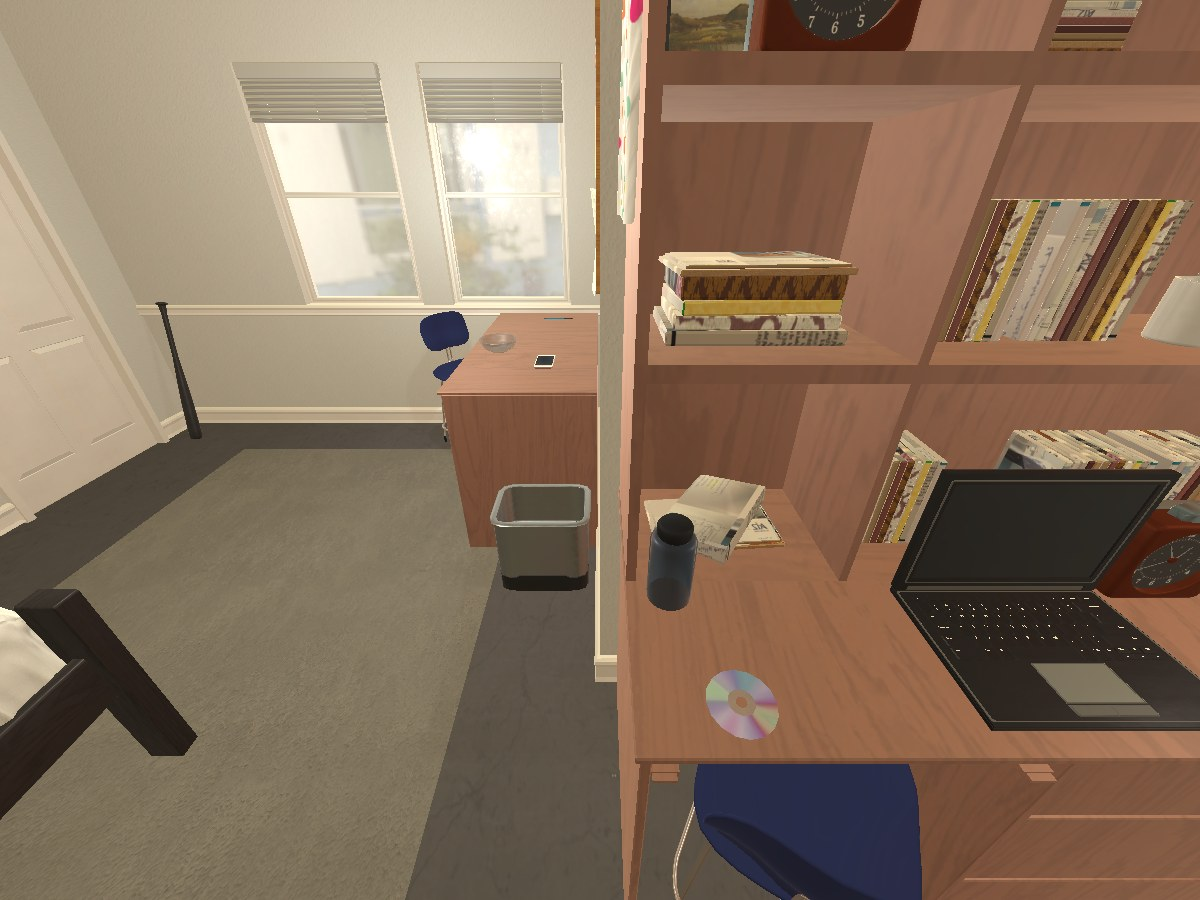
\includegraphics[width=8.508cm]{figures/cases/task0_view1.jpg}};
\draw[black!35, line width=0.4pt] (0.000,0.000) rectangle ++(8.508,-6.381);
\draw[dimF, line width=1.1pt] (8.295,-2.216) circle (0.302);
\draw[lead=dimF] (8.295,-2.216) -- (8.064,-1.754);
\fill[dimF] (8.295,-2.216) circle (0.06);
\node[lblkey=dimF] at (8.064,-1.754) {mug};
\draw[liftpositive, line width=1.1pt, rounded corners=1pt] (3.098,-2.226) rectangle (4.233,-3.878);
\draw[lead=liftpositive] (3.666,-3.052) -- (3.666,-2.552);
\fill[liftpositive] (3.666,-3.052) circle (0.06);
\node[lblkey=liftpositive] at (3.666,-2.552) {desk: put it here};
\draw[dimA, line width=1.1pt, rounded corners=1pt] (6.587,-0.624) rectangle (8.501,-2.581);
\draw[lead=dimA] (7.544,-1.602) -- (6.491,-1.249);
\fill[dimA] (7.544,-1.602) circle (0.06);
\node[lblkey=dimA] at (6.491,-1.249) {shelf: the mug is here};
\fill[black!55] (6.438,-4.931) circle (0.06);
\node[lbl=black!45] at (6.438,-4.931) {desk};
\draw[lead=black!55] (5.906,-1.602) -- (5.006,-1.794);
\fill[black!55] (5.906,-1.602) circle (0.06);
\node[lbl=black!45] at (5.006,-1.794) {shelves};
\fill[black!55] (0.698,-4.999) circle (0.06);
\node[lbl=black!45] at (0.698,-4.999) {bed};
\draw[lead=black!55] (7.675,-6.005) -- (7.675,-5.505);
\fill[black!55] (7.675,-6.005) circle (0.06);
\node[lbl=black!45] at (7.675,-5.505) {drawers};
\draw[lead=black!55] (3.829,-3.815) -- (3.829,-3.315);
\fill[black!55] (3.829,-3.815) circle (0.06);
\node[lbl=black!45] at (3.829,-3.315) {garbagecan};
\node[anchor=north west, inner sep=0] at (8.758,0.000) {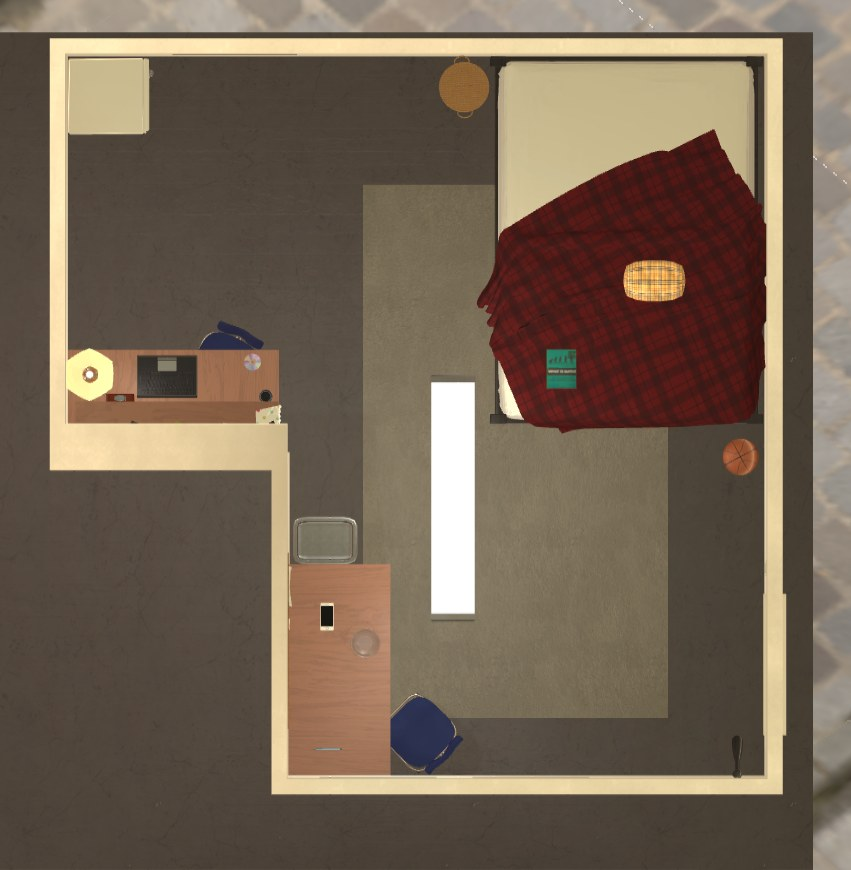
\includegraphics[width=6.242cm]{figures/cases/task0_map.jpg}};
\draw[black!35, line width=0.4pt] (8.758,0.000) rectangle ++(6.242,-6.381);
\fill[black, opacity=0.22] (10.861,-2.189) -- ++(-135:1.1) arc (-135:-45:1.1) -- cycle;
\fill[black] (10.861,-2.189) circle (0.08);
\draw[white, line width=3.4pt, opacity=0.85] (9.917,-3.289) -- (11.191,-4.899);
\draw[path] (9.917,-3.289) -- (11.191,-4.899);
\draw[lead=dimA] (9.792,-3.132) -- (10.845,-3.485);
\fill[dimA] (9.792,-3.132) circle (0.06);
\node[lblkey=dimA] at (10.845,-3.485) {shelf: the mug is here};
\draw[lead=liftpositive] (11.347,-5.095) -- (11.347,-4.595);
\fill[liftpositive] (11.347,-5.095) circle (0.06);
\node[lblkey=liftpositive] at (11.347,-4.595) {desk: put it here};
\draw[lead=black!55] (13.353,-1.719) -- (13.353,-1.219);
\fill[black!55] (13.353,-1.719) circle (0.06);
\node[lbl=black!45] at (13.353,-1.219) {bed};
\draw[lead=black!55] (10.211,-2.842) -- (10.211,-2.342);
\fill[black!55] (10.211,-2.842) circle (0.06);
\node[lbl=black!45] at (10.211,-2.342) {desk};
\draw[lead=black!55] (9.659,-2.774) -- (10.559,-2.965);
\fill[black!55] (9.659,-2.774) circle (0.06);
\node[lbl=black!45] at (10.559,-2.965) {drawers};
\draw[lead=black!55] (11.415,-4.542) -- (11.415,-4.042);
\fill[black!55] (11.415,-4.542) circle (0.06);
\node[lbl=black!45] at (11.415,-4.042) {drawers};
\draw[lead=black!55] (11.143,-3.966) -- (9.953,-3.966);
\fill[black!55] (11.143,-3.966) circle (0.06);
\node[lbl=black!45] at (9.953,-3.966) {garbagecan};
\draw[lead=black!55] (12.162,-0.638) -- (11.375,-0.285);
\fill[black!55] (12.162,-0.638) circle (0.06);
\node[lbl=black!45] at (11.375,-0.285) {laundryhamper};
\draw[lead=black!55] (9.536,-0.706) -- (9.296,-0.244);
\fill[black!55] (9.536,-0.706) circle (0.06);
\node[lbl=black!45] at (9.296,-0.244) {safe};
\draw[lead=black!55] (10.236,-3.132) -- (9.337,-2.941);
\fill[black!55] (10.236,-3.132) circle (0.06);
\node[lbl=black!45] at (9.337,-2.941) {shelves};
\node[imgcap] at (4.254,-6.421) {first-person view inside the room};
\node[imgcap] at (11.879,-6.421) {the room from above; cone: the left view; arrow: the expert's route};
\node[anchor=west, font=\sffamily\bfseries\footnotesize, text=black!70] at (0,-7.181) {Expert solution (4 steps):};
\node[chip, anchor=west] (s0) at (3.900,-7.181) {go to shelf};
\node[chip, anchor=west] (s1) at (6.162,-7.181) {take mug from shelf};
\draw[flow] (s0.east) -- (s1.west);
\node[chip, anchor=west] (s2) at (9.560,-7.181) {go to desk};
\draw[flow] (s1.east) -- (s2.west);
\node[chip, anchor=west] (s3) at (11.680,-7.181) {move mug to desk};
\draw[flow] (s2.east) -- (s3.west);
\node[ptitle] at (0.000,-7.981) {(b) What happened: \texttt{GPT-4o-mini}, seed 0};
\node[lab] at (1.650,-8.581) {expert};
\fill[black!30, rounded corners=1pt] (1.750,-8.431) rectangle ++(0.800,-0.3);
\node[txt] at (2.630,-8.581) {4};
\node[lab] at (1.650,-9.041) {no memory};
\fill[phaseA!35, rounded corners=1pt] (1.750,-8.891) rectangle ++(3.800,-0.3);
\node[txt] at (5.630,-9.041) {19, solved};
\node[lab] at (1.650,-9.501) {memory};
\fill[salmon!60, rounded corners=1pt] (1.750,-9.351) rectangle ++(1.200,-0.3);
\node[txt] at (3.030,-9.501) {6, solved};
\draw[densely dashed, black!40] (7.750,-8.331) -- (7.750,-9.761);
\node[font=\sffamily\scriptsize, text=black!50, anchor=north] at (7.750,-9.761) {30-step limit};
\node[txt] at (10.600,-8.581) {prompt tokens: 40,783 $\rightarrow$ 17,850};
\node[txt] at (10.600,-9.001) {effect over 3 demo pairs:};
\node[txt] at (10.600,-9.421) {\quad GPT $0.000$, Qwen $-0.333$};
\end{scope}
\end{tikzpicture}
}
\end{center}
\vspace{-4pt}
\captionof{figure}{Task 0. (a) The bedroom of this task, rendered from one of the two benchmark trials whose goal text matches the run log. The mug starts on a shelf of the desk hutch and must be moved to the other desk; the expert needs four steps. (b) \gptm on seed 0 solves the task in both conditions, in 19 steps without memory and 6 with it.}
\label{fig:case_task0}
\vspace{4pt}

\textbf{The task.} The agent starts in a bedroom and reads: \emph{``You are in the middle
of a room. Looking quickly around you, you see a bed 1, a desk 2, a desk 1, a drawer 6,
a drawer 5, a drawer 4, a drawer 3, a drawer 2, a drawer 1, a garbagecan 1, a
laundryhamper 1, a safe 1, a shelf 6, a shelf 5, a shelf 4, a shelf 3, a shelf 2, and a
shelf 1. Your task is to: put a mug in desk.''} The room has 18 places to look, and the
agent does not know where the mug is.

\textbf{What it takes.} In the benchmark data this goal exists as three trials in the
same room, and in all three the mug starts on a shelf. The expert solution is four
steps: \texttt{go to shelf}, \texttt{take mug from shelf}, \texttt{go to desk},
\texttt{move mug to desk}. A searching agent needs extra steps to find the right shelf.

\textbf{What the memory offers.} Two \texttt{[put]} demonstrations are in the prompt
in both conditions. With memory, the agent also reads all 33 insights; the first
\texttt{[put]} rule appears third. The six \texttt{[put]} rules (items 22--27) describe
a search-then-place routine, for example ``If the initial location does not contain the
target object, systematically explore other nearby locations'' and ``Ensure to confirm
the target object is in your possession before attempting to place it''. Notably, the
rule naming likely places lists ``tables, countertops, or drawers'', not shelves.

\textbf{What happened.} \gptm (seed 0) solves the task in both conditions: in 19 steps
with 40{,}783 prompt tokens without memory, and in 6 steps, two above the expert, with
17{,}850 prompt tokens with memory. Over the three demonstration pairs, \gptm's success
on this task is the same with and without memory (effect $0.000$). \qwenm solves it on
every pair without memory and fails one pair with memory ($-0.333$).

\textbf{Analysis.} The memory makes \gptm's successful search much more direct on this
task, from more than four times the expert length to near it, but because the task was
already solved, the success rate does not register the improvement. Without the step
trace we cannot tell which rule, if any, shortened the search. For \qwenm, which was at
ceiling on this task, the added block could only cost success, and it did on one pair.
Success-rate deltas therefore miss efficiency gains, and for a stack already at
ceiling they can only record losses.
\end{casebox}

\begin{casebox}[dimF]{Case 2 \textperiodcentered{} \texttt{heat} \textperiodcentered{} Task 1: ``heat some egg and put it in garbagecan''}
\begin{center}
\resizebox{\linewidth}{!}{\begin{tikzpicture}[x=1cm, y=1cm, font=\sffamily\footnotesize,
  ptitle/.style={anchor=west, font=\sffamily\bfseries\small, text=narrareddeep},
  textbox/.style={draw=phaseA!60, fill=phaseA!6, rounded corners=2pt, inner sep=4pt, anchor=north west,
                  align=left, font=\sffamily\scriptsize},
  lbl/.style={draw=#1, fill=white, fill opacity=0.9, text opacity=1, rounded corners=1pt, inner sep=1.6pt,
              line width=0.6pt, font=\sffamily\scriptsize},
  lblkey/.style={draw=#1, fill=white, fill opacity=0.95, text opacity=1, rounded corners=1pt, inner sep=1.8pt,
                 line width=1.0pt, font=\sffamily\scriptsize\bfseries},
  lead/.style={draw=#1, line width=0.7pt},
  path/.style={-{Latex[length=2.6mm, width=2.4mm]}, draw=black!85, line width=1.6pt},
  imgcap/.style={anchor=north, font=\sffamily\scriptsize, text=black!60},
  chip/.style={draw=black!30, fill=white, rounded corners=6pt, inner sep=2.5pt, font=\sffamily\footnotesize},
  flow/.style={-{Latex[length=1.6mm]}, draw=black!50, line width=0.6pt},
  lab/.style={anchor=east, font=\sffamily\footnotesize, text=black!75},
  txt/.style={anchor=west, font=\sffamily\footnotesize, text=black!75}]

\node[ptitle] at (0,0.000) {(a) The task and its room (AI2-THOR rendering of the benchmark trial)};
\node[textbox, text width=14.70cm] (obs) at (0,-0.280) {\textbf{Goal.} Your task is to: heat some egg and put it in garbagecan.\\[1pt]\textbf{Initial observation.} You are in the middle of a room. Looking quickly around you, you see a cabinet 6, a cabinet 5, a cabinet 4, a cabinet 3, a cabinet 2, a cabinet 1, a coffeemachine 1, a countertop 3, a countertop 2, a countertop 1, a drawer 3, a drawer 2, a drawer 1, a fridge 1, a garbagecan 1, a microwave 1, a shelf 3, a shelf 2, a shelf 1, a sinkbasin 1, a stoveburner 4, a stoveburner 3, a stoveburner 2, a stoveburner 1, and a toaster 1.};
\begin{scope}[shift={($(obs.south west)+(0,-0.25)$)}]
\node[anchor=north west, inner sep=0] at (0.000,0.000) {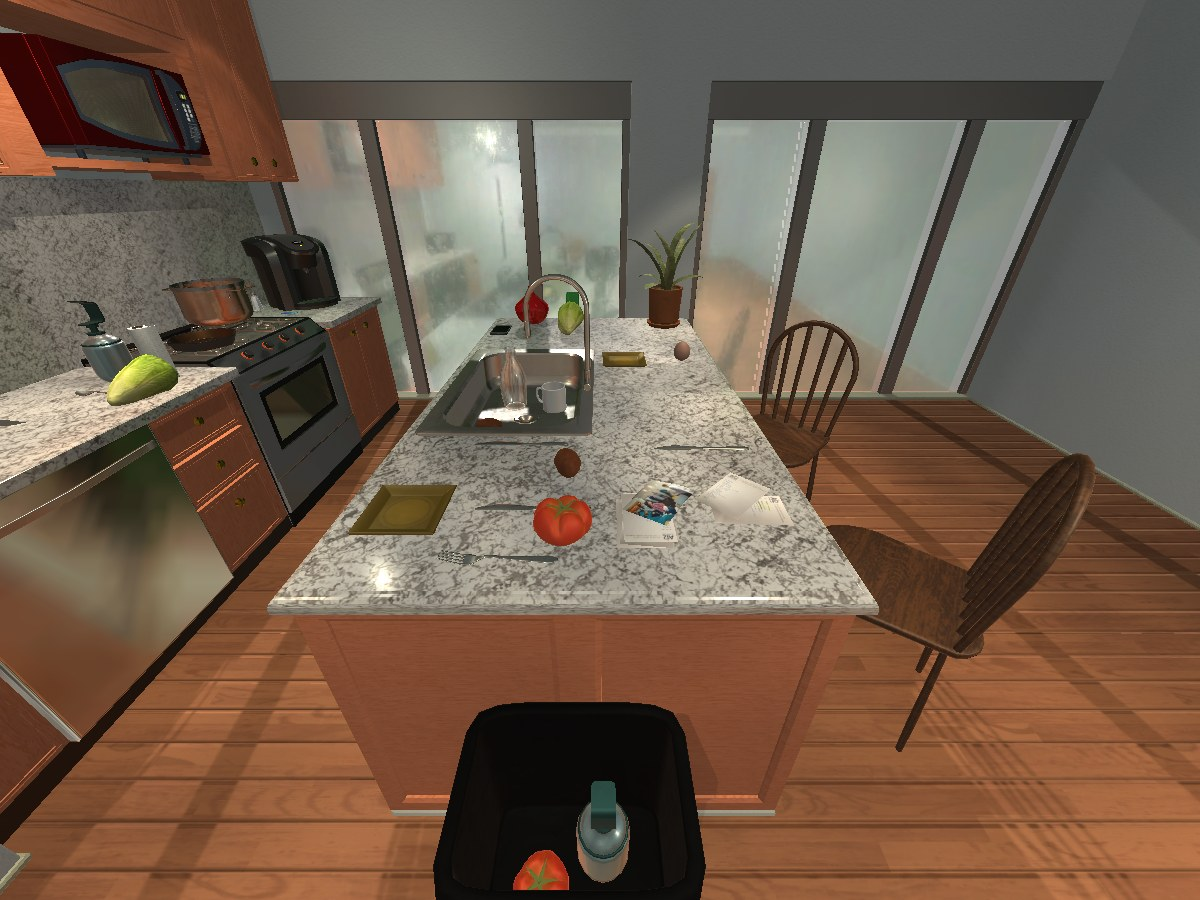
\includegraphics[width=8.815cm]{figures/cases/task1_view1.jpg}};
\draw[black!35, line width=0.4pt] (0.000,0.000) rectangle ++(8.815,-6.611);
\draw[dimF, line width=1.1pt] (5.006,-2.582) circle (0.160);
\draw[lead=dimF] (5.006,-2.582) -- (5.006,-2.082);
\fill[dimF] (5.006,-2.582) circle (0.06);
\node[lblkey=dimF] at (5.006,-2.082) {egg};
\draw[liftpositive, line width=1.1pt, rounded corners=1pt] (3.181,-5.164) rectangle (5.179,-6.611);
\draw[lead=liftpositive] (4.180,-5.888) -- (4.180,-5.388);
\fill[liftpositive] (4.180,-5.888) circle (0.06);
\node[lblkey=liftpositive] at (4.180,-5.388) {garbagecan: put it here};
\draw[dimA, line width=1.1pt, rounded corners=1pt] (2.101,-2.343) rectangle (6.325,-4.334);
\fill[dimA] (4.213,-3.339) circle (0.06);
\node[lblkey=dimA] at (4.213,-3.339) {countertop: the egg is here};
\draw[dimE, line width=1.1pt, rounded corners=1pt] (0.000,-0.250) rectangle (1.535,-1.212);
\draw[lead=dimE] (0.768,-0.731) -- (1.850,-1.084);
\fill[dimE] (0.768,-0.731) circle (0.06);
\node[lblkey=dimE] at (1.850,-1.084) {microwave: heat it here};
\draw[lead=black!55] (0.859,-3.122) -- (0.859,-2.622);
\fill[black!55] (0.859,-3.122) circle (0.06);
\node[lbl=black!45] at (0.859,-2.622) {countertops};
\draw[lead=black!55] (1.723,-0.668) -- (1.083,-0.315);
\fill[black!55] (1.723,-0.668) circle (0.06);
\node[lbl=black!45] at (1.083,-0.315) {cabinets};
\draw[lead=black!55] (1.763,-3.809) -- (1.763,-3.309);
\fill[black!55] (1.763,-3.809) circle (0.06);
\node[lbl=black!45] at (1.763,-3.309) {drawers};
\draw[lead=black!55] (2.130,-2.005) -- (2.130,-1.505);
\fill[black!55] (2.130,-2.005) circle (0.06);
\node[lbl=black!45] at (2.130,-1.505) {coffeemachine};
\node[anchor=north west, inner sep=0] at (9.065,0.000) {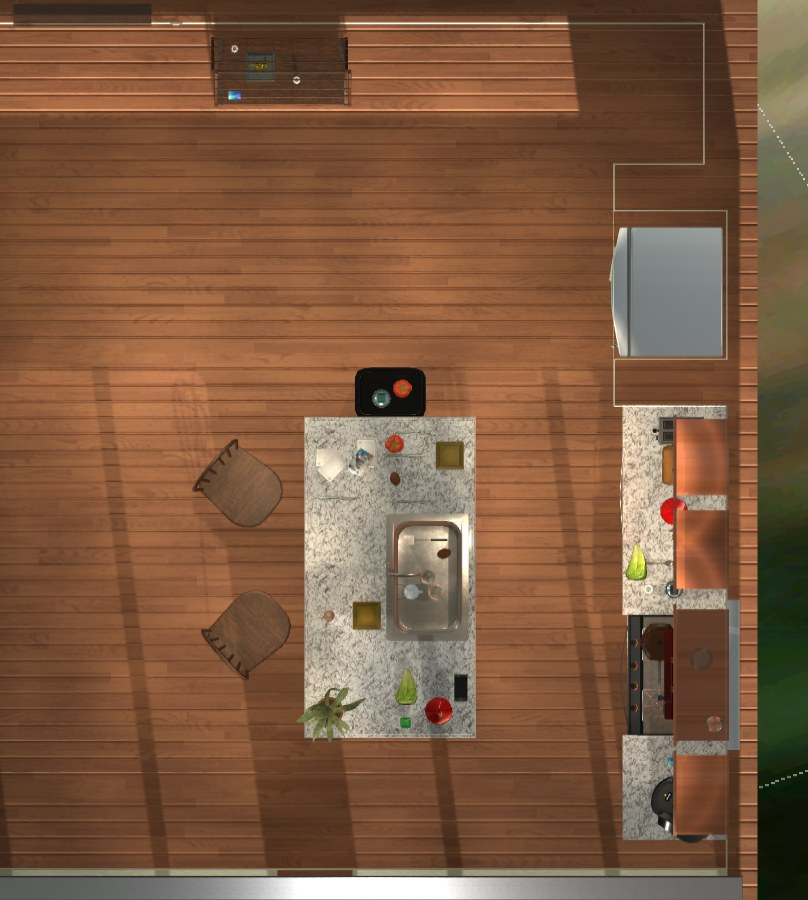
\includegraphics[width=5.935cm]{figures/cases/task1_map.jpg}};
\draw[black!35, line width=0.4pt] (9.065,0.000) rectangle ++(5.935,-6.611);
\fill[black, opacity=0.22] (11.874,-2.424) -- ++(-135:1.1) arc (-135:-45:1.1) -- cycle;
\fill[black] (11.874,-2.424) circle (0.08);
\draw[white, line width=3.4pt, opacity=0.85] (11.804,-4.290) -- (13.885,-4.885);
\draw[path] (11.804,-4.290) -- (13.885,-4.885);
\draw[white, line width=3.4pt, opacity=0.85] (13.979,-4.817) -- (12.115,-3.063);
\draw[path] (13.979,-4.817) -- (12.115,-3.063);
\draw[lead=dimA] (11.611,-4.235) -- (11.611,-3.735);
\fill[dimA] (11.611,-4.235) circle (0.06);
\node[lblkey=dimA] at (11.611,-3.735) {countertop: the egg is here};
\draw[lead=dimE] (14.125,-4.954) -- (13.043,-4.600);
\fill[dimE] (14.125,-4.954) circle (0.06);
\node[lblkey=dimE] at (13.043,-4.600) {microwave: heat it here};
\draw[lead=liftpositive] (11.933,-2.891) -- (10.851,-3.245);
\fill[liftpositive] (11.933,-2.891) circle (0.06);
\node[lblkey=liftpositive] at (10.851,-3.245) {garbagecan: put it here};
\draw[lead=black!55] (13.912,-3.766) -- (13.912,-3.266);
\fill[black!55] (13.912,-3.766) circle (0.06);
\node[lbl=black!45] at (13.912,-3.266) {cabinets};
\draw[lead=black!55] (13.912,-5.682) -- (13.912,-5.182);
\fill[black!55] (13.912,-5.682) circle (0.06);
\node[lbl=black!45] at (13.912,-5.182) {cabinets};
\draw[lead=black!55] (14.098,-5.925) -- (12.896,-5.734);
\fill[black!55] (14.098,-5.925) circle (0.06);
\node[lbl=black!45] at (12.896,-5.734) {coffeemachine};
\draw[lead=black!55] (14.003,-3.755) -- (14.003,-2.655);
\fill[black!55] (14.003,-3.755) circle (0.06);
\node[lbl=black!45] at (14.003,-2.655) {countertop};
\draw[lead=black!55] (14.003,-5.786) -- (13.305,-6.140);
\fill[black!55] (14.003,-5.786) circle (0.06);
\node[lbl=black!45] at (13.305,-6.140) {countertop};
\draw[lead=black!55] (13.679,-4.242) -- (14.289,-3.889);
\fill[black!55] (13.679,-4.242) circle (0.06);
\node[lbl=black!45] at (14.289,-3.889) {drawers};
\draw[lead=black!55] (14.041,-2.144) -- (14.041,-1.644);
\fill[black!55] (14.041,-2.144) circle (0.06);
\node[lbl=black!45] at (14.041,-1.644) {fridge};
\draw[lead=black!55] (11.115,-0.530) -- (10.215,-0.339);
\fill[black!55] (11.115,-0.530) circle (0.06);
\node[lbl=black!45] at (10.215,-0.339) {shelves};
\draw[lead=black!55] (12.207,-4.239) -- (10.776,-4.239);
\fill[black!55] (12.207,-4.239) circle (0.06);
\node[lbl=black!45] at (10.776,-4.239) {sinkbasin};
\draw[lead=black!55] (14.034,-4.960) -- (12.852,-4.182);
\fill[black!55] (14.034,-4.960) circle (0.06);
\node[lbl=black!45] at (12.852,-4.182) {stoveburners};
\draw[lead=black!55] (14.060,-3.164) -- (14.060,-2.064);
\fill[black!55] (14.060,-3.164) circle (0.06);
\node[lbl=black!45] at (14.060,-2.064) {toaster};
\node[imgcap] at (4.407,-6.651) {first-person view inside the room};
\node[imgcap] at (12.032,-6.651) {the room from above; cone: the left view; arrow: the expert's route};
\node[anchor=west, font=\sffamily\bfseries\footnotesize, text=black!70] at (0,-7.411) {Expert solution (6 steps):};
\node[chip, anchor=west] (s0) at (3.900,-7.411) {go to countertop};
\node[chip, anchor=west] (s1) at (6.872,-7.411) {take egg from countertop};
\draw[flow] (s0.east) -- (s1.west);
\node[chip, anchor=west] (s2) at (10.980,-7.411) {go to microwave};
\draw[flow] (s1.east) -- (s2.west);
\node[chip, anchor=west] (s3) at (3.900,-7.911) {heat egg with microwave};
\node[chip, anchor=west] (s4) at (7.866,-7.911) {go to garbagecan};
\draw[flow] (s3.east) -- (s4.west);
\node[chip, anchor=west] (s5) at (10.838,-7.911) {move egg to garbagecan};
\draw[flow] (s4.east) -- (s5.west);
\node[ptitle] at (0.000,-8.711) {(b) What happened: \texttt{GPT-4o-mini}, seed 0};
\node[lab] at (1.650,-9.311) {expert};
\fill[black!30, rounded corners=1pt] (1.750,-9.161) rectangle ++(1.200,-0.3);
\node[txt] at (3.030,-9.311) {6};
\node[lab] at (1.650,-9.771) {no memory};
\fill[phaseA!35, rounded corners=1pt] (1.750,-9.621) rectangle ++(6.000,-0.3);
\node[txt] at (7.830,-9.771) {30, not solved};
\node[lab] at (1.650,-10.231) {memory};
\fill[salmon!60, rounded corners=1pt] (1.750,-10.081) rectangle ++(6.000,-0.3);
\node[txt] at (7.830,-10.231) {30, not solved};
\draw[densely dashed, black!40] (7.750,-9.061) -- (7.750,-10.491);
\node[font=\sffamily\scriptsize, text=black!50, anchor=north] at (7.750,-10.491) {30-step limit};
\node[txt] at (10.600,-9.311) {prompt tokens: 81,372 $\rightarrow$ 108,358};
\node[txt] at (10.600,-9.731) {effect over 3 demo pairs:};
\node[txt] at (10.600,-10.151) {\quad GPT $0.000$, Qwen $-0.333$};
\end{scope}
\end{tikzpicture}
}
\end{center}
\vspace{-4pt}
\captionof{figure}{Task 1. (a) The kitchen, rendered from a trial in which the egg starts on a countertop (two of the three trials of this goal; in the third it starts in the garbage can). The egg must be heated in the microwave and then put in the garbage can. (b) \gptm on seed 0 reaches the 30-step limit in both conditions.}
\label{fig:case_task1}
\vspace{4pt}

\textbf{The task.} The agent starts in a kitchen: \emph{``\ldots you see a cabinet 6,
a cabinet 5, a cabinet 4, a cabinet 3, a cabinet 2, a cabinet 1, a coffeemachine 1, a
countertop 3, a countertop 2, a countertop 1, a drawer 3, a drawer 2, a drawer 1, a
fridge 1, a garbagecan 1, a microwave 1, a shelf 3, a shelf 2, a shelf 1, a sinkbasin 1,
a stoveburner 4, a stoveburner 3, a stoveburner 2, a stoveburner 1, and a toaster 1.
Your task is to: heat some egg and put it in garbagecan.''} There are 25 places to look.

\textbf{What it takes.} The egg starts on a countertop in two of the three trials of
this goal and inside the garbage can in the third. The expert solution is six steps:
go to the egg, take it, \texttt{go to microwave}, \texttt{heat egg with microwave},
\texttt{go to garbagecan}, \texttt{move egg to garbagecan}.

\textbf{What the memory offers.} Here the first \texttt{[heat]} rule is the
\emph{first} item of the memory block, so the matching procedure is as salient as it
can be. The five \texttt{[heat]} rules (items 17--21) include ``Use appropriate
appliances or tools to modify the item as needed before completing the task'' and
``Ensure to open or interact with containers before placing or retrieving items''.

\textbf{What happened.} \gptm (seed 0) fails in both conditions, stopping at the
30-step limit, five times the expert length. The memory raises the episode's prompt
tokens from 81{,}372 to 108{,}358. Over the three pairs, \gptm's success on this task is
unchanged ($0.000$), while \qwenm, which solved it on one pair without memory, loses
that pair ($-0.333$).

\textbf{Analysis.} \texttt{heat} is \gptm's weakest family ($0.130$ without memory)
and the one where the memory helps it most after \texttt{puttwo} ($+0.246$), so this
task is a counterexample inside a strong family gain: the most relevant rule comes
first and the agent still fails, at a 33\% higher token cost. The rules state the
generic procedure (find, use the appliance, place) but nothing about where an egg is,
which is what the agent must discover. Task 133, another \texttt{heat} task with its
first rule also at rank~1, shows the family's other face: \gptm $+0.833$, \qwenm
$-0.333$ from a \qwenm no-memory success of $1.000$.
\end{casebox}

\begin{casebox}[dimD]{Case 3 \textperiodcentered{} \texttt{puttwo} \textperiodcentered{} Task 2: ``put two pillow in sofa''}
\begin{center}
\resizebox{\linewidth}{!}{\begin{tikzpicture}[x=1cm, y=1cm, font=\sffamily\footnotesize,
  ptitle/.style={anchor=west, font=\sffamily\bfseries\small, text=narrareddeep},
  textbox/.style={draw=phaseA!60, fill=phaseA!6, rounded corners=2pt, inner sep=4pt, anchor=north west,
                  align=left, font=\sffamily\scriptsize},
  lbl/.style={draw=#1, fill=white, fill opacity=0.9, text opacity=1, rounded corners=1pt, inner sep=1.6pt,
              line width=0.6pt, font=\sffamily\scriptsize},
  lblkey/.style={draw=#1, fill=white, fill opacity=0.95, text opacity=1, rounded corners=1pt, inner sep=1.8pt,
                 line width=1.0pt, font=\sffamily\scriptsize\bfseries},
  lead/.style={draw=#1, line width=0.7pt},
  path/.style={-{Latex[length=2.6mm, width=2.4mm]}, draw=black!85, line width=1.6pt},
  imgcap/.style={anchor=north, font=\sffamily\scriptsize, text=black!60},
  chip/.style={draw=black!30, fill=white, rounded corners=6pt, inner sep=2.5pt, font=\sffamily\footnotesize},
  flow/.style={-{Latex[length=1.6mm]}, draw=black!50, line width=0.6pt},
  lab/.style={anchor=east, font=\sffamily\footnotesize, text=black!75},
  txt/.style={anchor=west, font=\sffamily\footnotesize, text=black!75}]

\node[ptitle] at (0,0.000) {(a) The task and its room (AI2-THOR rendering of the benchmark trial)};
\node[textbox, text width=14.70cm] (obs) at (0,-0.280) {\textbf{Goal.} Your task is to: put two pillow in sofa.\\[1pt]\textbf{Initial observation.} You are in the middle of a room. Looking quickly around you, you see a armchair 1, a cabinet 4, a cabinet 3, a cabinet 2, a cabinet 1, a drawer 5, a drawer 4, a drawer 3, a drawer 2, a drawer 1, a dresser 1, a garbagecan 1, a safe 1, a shelf 12, a shelf 11, a shelf 10, a shelf 9, a shelf 8, a shelf 7, a shelf 6, a shelf 5, a shelf 4, a shelf 3, a shelf 2, a shelf 1, a sidetable 1, and a sofa 1.};
\begin{scope}[shift={($(obs.south west)+(0,-0.25)$)}]
\node[anchor=north west, inner sep=0] at (0.000,0.000) {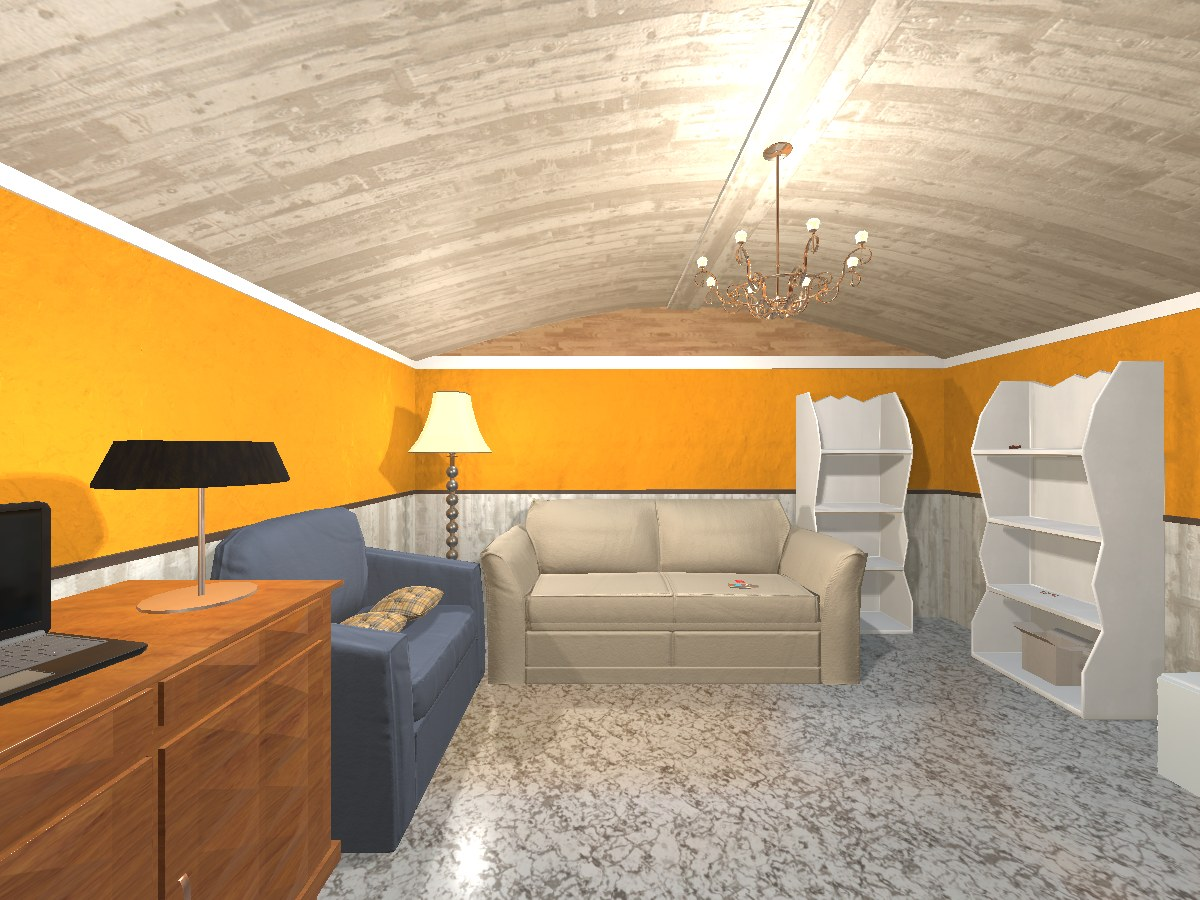
\includegraphics[width=7.919cm]{figures/cases/task2_view1.jpg}};
\draw[black!35, line width=0.4pt] (0.000,0.000) rectangle ++(7.919,-5.939);
\draw[dimF, line width=1.1pt] (2.462,-4.108) circle (0.261);
\draw[lead=dimF] (2.462,-4.108) -- (2.462,-3.608);
\fill[dimF] (2.462,-4.108) circle (0.06);
\node[lblkey=dimF] at (2.462,-3.608) {pillow};
\draw[dimF, line width=1.1pt] (2.683,-3.986) circle (0.289);
\draw[lead=dimF] (2.683,-3.986) -- (1.833,-4.177);
\fill[dimF] (2.683,-3.986) circle (0.06);
\node[lblkey=dimF] at (1.833,-4.177) {pillow};
\draw[dimA, line width=1.1pt, rounded corners=1pt] (1.386,-3.352) rectangle (3.201,-5.629);
\draw[lead=dimA] (2.293,-4.491) -- (2.293,-4.991);
\fill[dimA] (2.293,-4.491) circle (0.06);
\node[lblkey=dimA] at (2.293,-4.991) {armchair: the pillows are here};
\draw[liftpositive, line width=1.1pt, rounded corners=1pt] (3.168,-3.293) rectangle (5.722,-4.521);
\fill[liftpositive] (4.445,-3.907) circle (0.06);
\node[lblkey=liftpositive] at (4.445,-3.907) {sofa: put both here};
\draw[lead=black!55] (1.132,-4.887) -- (0.751,-4.148);
\fill[black!55] (1.132,-4.887) circle (0.06);
\node[lbl=black!45] at (0.751,-4.148) {dresser};
\fill[black!55] (7.045,-3.570) circle (0.06);
\node[lbl=black!45] at (7.045,-3.570) {shelves};
\draw[lead=black!55] (1.584,-5.085) -- (1.584,-4.585);
\fill[black!55] (1.584,-5.085) circle (0.06);
\node[lbl=black!45] at (1.584,-4.585) {cabinets};
\draw[lead=black!55] (0.505,-5.012) -- (0.771,-5.474);
\fill[black!55] (0.505,-5.012) circle (0.06);
\node[lbl=black!45] at (0.771,-5.474) {drawers};
\node[anchor=north west, inner sep=0] at (8.169,0.000) {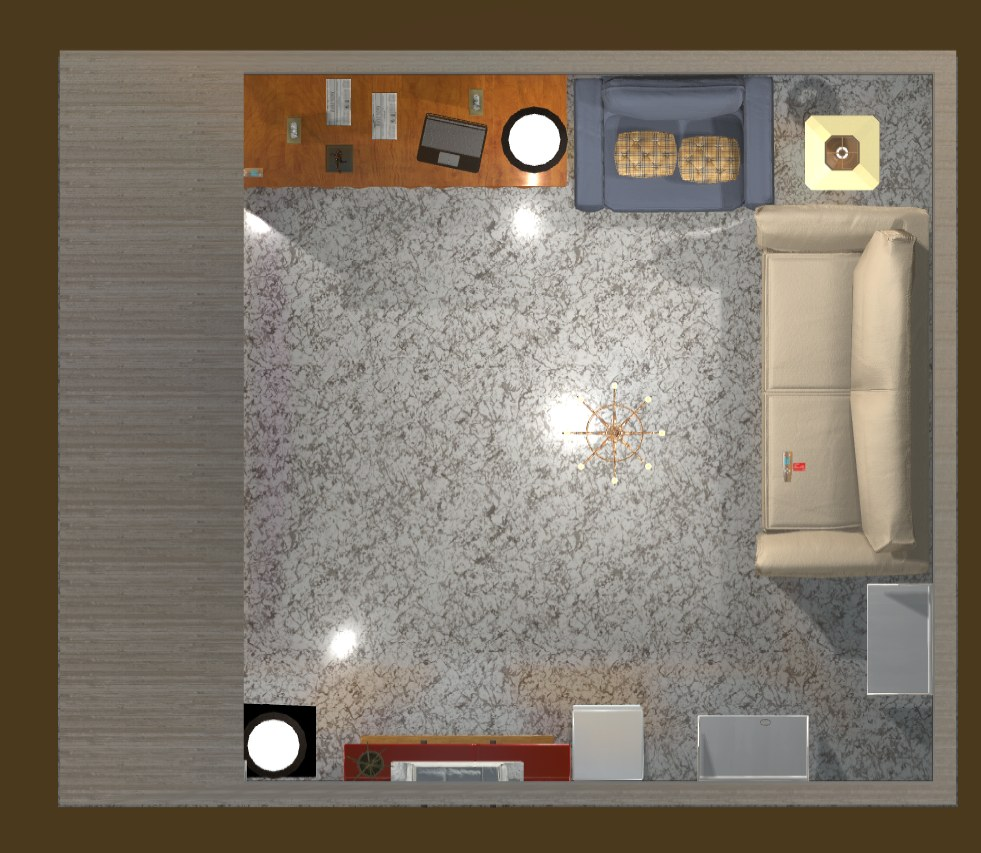
\includegraphics[width=6.831cm]{figures/cases/task2_map.jpg}};
\draw[black!35, line width=0.4pt] (8.169,0.000) rectangle ++(6.831,-5.939);
\fill[black, opacity=0.22] (10.468,-2.234) -- ++(-45:1.1) arc (-45:45:1.1) -- cycle;
\fill[black] (10.468,-2.234) circle (0.08);
\draw[white, line width=3.4pt, opacity=0.85] (12.967,-1.160) -- (13.815,-2.515);
\draw[path] (12.967,-1.160) -- (13.815,-2.515);
\draw[lead=dimA] (12.861,-0.991) -- (12.861,-0.491);
\fill[dimA] (12.861,-0.991) circle (0.06);
\node[lblkey=dimA] at (12.861,-0.491) {armchair: the pillows are here};
\draw[lead=liftpositive] (13.948,-2.727) -- (13.578,-2.265);
\fill[liftpositive] (13.948,-2.727) circle (0.06);
\node[lblkey=liftpositive] at (13.578,-2.265) {sofa: put both here};
\draw[lead=black!55] (10.471,-1.290) -- (10.195,-0.828);
\fill[black!55] (10.471,-1.290) circle (0.06);
\node[lbl=black!45] at (10.195,-0.828) {cabinets};
\draw[lead=black!55] (12.003,-1.290) -- (11.393,-0.936);
\fill[black!55] (12.003,-1.290) circle (0.06);
\node[lbl=black!45] at (11.393,-0.936) {cabinet};
\draw[lead=black!55] (11.139,-1.191) -- (10.239,-1.383);
\fill[black!55] (11.139,-1.191) circle (0.06);
\node[lbl=black!45] at (10.239,-1.383) {drawers};
\draw[lead=black!55] (9.982,-1.191) -- (9.028,-1.191);
\fill[black!55] (9.982,-1.191) circle (0.06);
\node[lbl=black!45] at (9.028,-1.191) {drawer};
\draw[lead=black!55] (9.700,-5.087) -- (9.700,-4.587);
\fill[black!55] (9.700,-5.087) circle (0.06);
\node[lbl=black!45] at (9.700,-4.587) {drawer};
\draw[lead=black!55] (10.851,-0.908) -- (10.029,-0.342);
\fill[black!55] (10.851,-0.908) circle (0.06);
\node[lbl=black!45] at (10.029,-0.342) {dresser};
\draw[lead=black!55] (8.937,-1.418) -- (8.937,-1.918);
\fill[black!55] (8.937,-1.418) circle (0.06);
\node[lbl=black!45] at (8.937,-1.918) {garbagecan};
\draw[lead=black!55] (12.402,-5.188) -- (12.402,-4.688);
\fill[black!55] (12.402,-5.188) circle (0.06);
\node[lbl=black!45] at (12.402,-4.688) {safe};
\draw[lead=black!55] (13.917,-4.839) -- (13.917,-4.339);
\fill[black!55] (13.917,-4.839) circle (0.06);
\node[lbl=black!45] at (13.917,-4.339) {shelves};
\draw[lead=black!55] (9.487,-5.379) -- (8.877,-5.025);
\fill[black!55] (9.487,-5.379) circle (0.06);
\node[lbl=black!45] at (8.877,-5.025) {shelves};
\draw[lead=black!55] (9.700,-5.189) -- (9.031,-5.542);
\fill[black!55] (9.700,-5.189) circle (0.06);
\node[lbl=black!45] at (9.031,-5.542) {sidetable};
\node[imgcap] at (3.960,-5.979) {first-person view inside the room};
\node[imgcap] at (11.585,-5.979) {the room from above; cone: the left view; arrow: the expert's route};
\node[anchor=west, font=\sffamily\bfseries\footnotesize, text=black!70] at (0,-6.739) {Expert solution (8 steps):};
\node[chip, anchor=west] (s0) at (3.900,-6.739) {go to armchair};
\node[chip, anchor=west] (s1) at (6.588,-6.739) {take pillow from armchair};
\draw[flow] (s0.east) -- (s1.west);
\node[chip, anchor=west] (s2) at (10.838,-6.739) {go to sofa};
\draw[flow] (s1.east) -- (s2.west);
\node[chip, anchor=west] (s3) at (3.900,-7.239) {move pillow to sofa};
\node[chip, anchor=west] (s4) at (7.298,-7.239) {go to armchair};
\draw[flow] (s3.east) -- (s4.west);
\node[chip, anchor=west] (s5) at (9.986,-7.239) {take pillow from armchair};
\draw[flow] (s4.east) -- (s5.west);
\node[chip, anchor=west] (s6) at (3.900,-7.739) {go to sofa};
\node[chip, anchor=west] (s7) at (6.020,-7.739) {move pillow to sofa};
\draw[flow] (s6.east) -- (s7.west);
\node[ptitle] at (0.000,-8.539) {(b) What happened: \texttt{GPT-4o-mini}, seed 0};
\node[lab] at (1.650,-9.139) {expert};
\fill[black!30, rounded corners=1pt] (1.750,-8.989) rectangle ++(1.600,-0.3);
\node[txt] at (3.430,-9.139) {8};
\node[lab] at (1.650,-9.599) {no memory};
\fill[phaseA!35, rounded corners=1pt] (1.750,-9.449) rectangle ++(6.000,-0.3);
\node[txt] at (7.830,-9.599) {30, not solved};
\node[lab] at (1.650,-10.059) {memory};
\fill[salmon!60, rounded corners=1pt] (1.750,-9.909) rectangle ++(6.000,-0.3);
\node[txt] at (7.830,-10.059) {30, not solved};
\draw[densely dashed, black!40] (7.750,-8.889) -- (7.750,-10.319);
\node[font=\sffamily\scriptsize, text=black!50, anchor=north] at (7.750,-10.319) {30-step limit};
\node[txt] at (10.600,-9.139) {prompt tokens: 89,011 $\rightarrow$ 109,495};
\node[txt] at (10.600,-9.559) {effect over 3 demo pairs:};
\node[txt] at (10.600,-9.979) {\quad not reported for this task};
\end{scope}
\end{tikzpicture}
}
\end{center}
\vspace{-4pt}
\captionof{figure}{Task 2. (a) The living room, rendered from one of the two trials whose goal text matches the run log. Both pillows start on the armchair and must be moved to the sofa, so the expert repeats one four-step routine. (b) \gptm on seed 0 reaches the 30-step limit in both conditions.}
\label{fig:case_task2}
\vspace{4pt}

\textbf{The task.} The agent starts in a living room with 27 places to look:
\emph{``\ldots you see a armchair 1, a cabinet 4, a cabinet 3, a cabinet 2, a cabinet 1,
a drawer 5, a drawer 4, a drawer 3, a drawer 2, a drawer 1, a dresser 1, a garbagecan 1,
a safe 1, a shelf 12, \ldots, a shelf 1, a sidetable 1, and a sofa 1. Your task is to:
put two pillow in sofa.''}

\textbf{What it takes.} In all three trials of this goal both pillows start on the
armchair. The expert solution is eight steps, the same four-step routine performed
twice: \texttt{go to armchair}, \texttt{take pillow from armchair}, \texttt{go to sofa},
\texttt{move pillow to sofa}.

\textbf{What the memory offers.} The five \texttt{[puttwo]} rules (items 28--32) speak
directly to the difficulty of the family, which is keeping track of the second instance:
``Once an item is found, immediately plan the next steps to retrieve and place it'',
``If the first search does not yield results, revisit previously checked locations, as
items may be present in multiple instances'', and ``Keep track of items already found
and placed to avoid unnecessary repetition in searches''. The first \texttt{[puttwo]}
rule is ranked 4th for the family's representative tasks.

\textbf{What happened.} \gptm (seed 0) fails in both conditions at the 30-step limit,
nearly four times the expert length, and the memory raises prompt tokens from
89{,}011 to 109{,}495. This task is not among the representative cases of
Table~\ref{tab:taxonomy}, so its equal-pair effects are not reported.

\textbf{Analysis.} Even with rules that name the exact difficulty and an expert path
that needs only one location, \gptm does not finish this task within the budget on
seed 0. Across the family, however, the memory lifts \gptm more than any other family
($0.333\rightarrow0.588$) while leaving \qwenm exactly unchanged
($0.431\rightarrow0.431$); two representative tasks move in opposite directions for
the two stacks (task 103: \gptm $+1.000$, \qwenm $0.000$; task 118: \gptm $-0.333$,
\qwenm $+0.333$). The transport gap is therefore visible inside a single family.
\end{casebox}

\noindent
The goals of the remaining representative tasks were not retained in the run logs, so
Cases~4--6 describe each family through the benchmark data and identify its
representative tasks by ID. Their figures show an example task of the family instead.

\begin{casebox}[dimC]{Case 4 \textperiodcentered{} \texttt{clean} \textperiodcentered{} family of 31 tasks; representative task 30}
\begin{center}
\resizebox{\linewidth}{!}{\begin{tikzpicture}[x=1cm, y=1cm, font=\sffamily\footnotesize,
  ptitle/.style={anchor=west, font=\sffamily\bfseries\small, text=narrareddeep},
  textbox/.style={draw=phaseA!60, fill=phaseA!6, rounded corners=2pt, inner sep=4pt, anchor=north west,
                  align=left, font=\sffamily\scriptsize},
  lbl/.style={draw=#1, fill=white, fill opacity=0.9, text opacity=1, rounded corners=1pt, inner sep=1.6pt,
              line width=0.6pt, font=\sffamily\scriptsize},
  lblkey/.style={draw=#1, fill=white, fill opacity=0.95, text opacity=1, rounded corners=1pt, inner sep=1.8pt,
                 line width=1.0pt, font=\sffamily\scriptsize\bfseries},
  lead/.style={draw=#1, line width=0.7pt},
  path/.style={-{Latex[length=2.6mm, width=2.4mm]}, draw=black!85, line width=1.6pt},
  imgcap/.style={anchor=north, font=\sffamily\scriptsize, text=black!60},
  chip/.style={draw=black!30, fill=white, rounded corners=6pt, inner sep=2.5pt, font=\sffamily\footnotesize},
  flow/.style={-{Latex[length=1.6mm]}, draw=black!50, line width=0.6pt},
  lab/.style={anchor=east, font=\sffamily\footnotesize, text=black!75},
  txt/.style={anchor=west, font=\sffamily\footnotesize, text=black!75}]

\node[ptitle] at (0,0.000) {(a) An example task of this family and its room (AI2-THOR rendering)};
\node[textbox, text width=14.70cm] (obs) at (0,-0.280) {\textbf{Goal.} Your task is to: put a clean soapbar in countertop.\\[1pt]\textbf{Initial observation.} You are in the middle of a room. Looking quickly around you, you see a cabinet 4, a cabinet 3, a cabinet 2, a cabinet 1, a countertop 1, a garbagecan 1, a handtowelholder 2, a handtowelholder 1, a sinkbasin 2, a sinkbasin 1, a toilet 1, a toiletpaperhanger 1, and a towelholder 1.};
\begin{scope}[shift={($(obs.south west)+(0,-0.25)$)}]
\node[anchor=north west, inner sep=0] at (0.000,0.000) {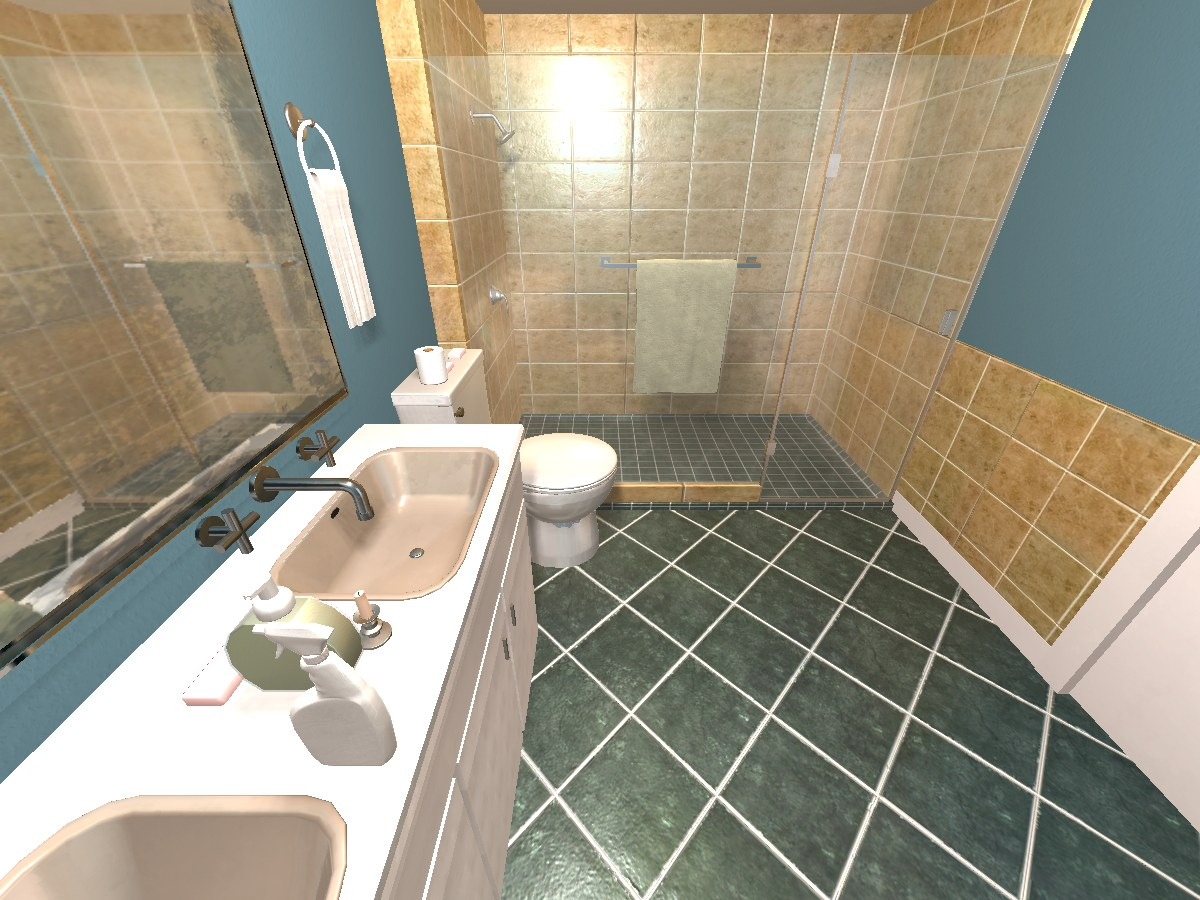
\includegraphics[width=9.012cm]{figures/cases/clean_view1.jpg}};
\draw[black!35, line width=0.4pt] (0.000,0.000) rectangle ++(9.012,-6.759);
\draw[dimF, line width=1.1pt] (3.428,-2.658) circle (0.160);
\draw[lead=dimF] (3.428,-2.658) -- (3.428,-2.158);
\fill[dimF] (3.428,-2.658) circle (0.06);
\node[lblkey=dimF] at (3.428,-2.158) {soapbar};
\draw[dimE, line width=1.1pt, rounded corners=1pt] (0.000,-5.978) rectangle (2.598,-6.759);
\draw[lead=dimE] (1.299,-6.368) -- (3.315,-6.368);
\fill[dimE] (1.299,-6.368) circle (0.06);
\node[lblkey=dimE] at (3.315,-6.368) {sinkbasin: clean it here};
\draw[liftpositive, line width=1.1pt, rounded corners=1pt] (0.000,-3.192) rectangle (3.905,-6.759);
\fill[liftpositive] (1.953,-4.975) circle (0.06);
\node[lblkey=liftpositive] at (1.953,-4.975) {countertop: put it here};
\draw[dimA, line width=1.1pt, rounded corners=1pt] (2.936,-2.628) rectangle (4.634,-4.266);
\draw[lead=dimA] (3.785,-3.447) -- (3.785,-2.947);
\fill[dimA] (3.785,-3.447) circle (0.06);
\node[lblkey=dimA] at (3.785,-2.947) {toilet: the soapbar is here};
\draw[lead=black!55] (2.880,-3.935) -- (2.880,-3.435);
\fill[black!55] (2.880,-3.935) circle (0.06);
\node[lbl=black!45] at (2.880,-3.435) {sinkbasin};
\draw[lead=black!55] (3.665,-5.610) -- (2.715,-5.418);
\fill[black!55] (3.665,-5.610) circle (0.06);
\node[lbl=black!45] at (2.715,-5.418) {cabinets};
\node[anchor=north west, inner sep=0] at (9.262,0.000) {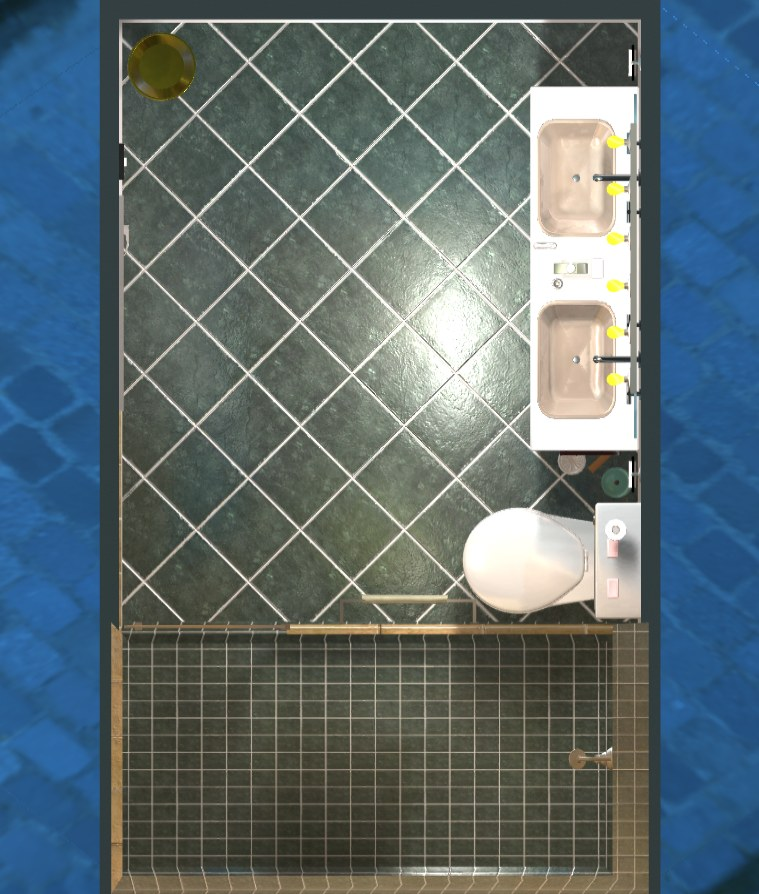
\includegraphics[width=5.738cm]{figures/cases/clean_map.jpg}};
\draw[black!35, line width=0.4pt] (9.262,0.000) rectangle ++(5.738,-6.759);
\fill[black, opacity=0.22] (12.888,-1.368) -- ++(-135:1.1) arc (-135:-45:1.1) -- cycle;
\fill[black] (12.888,-1.368) circle (0.08);
\draw[white, line width=3.4pt, opacity=0.85] (13.251,-4.028) -- (13.577,-1.589);
\draw[path] (13.251,-4.028) -- (13.577,-1.589);
\draw[white, line width=3.4pt, opacity=0.85] (13.631,-1.540) -- (13.656,-1.782);
\draw[path] (13.631,-1.540) -- (13.656,-1.782);
\draw[lead=dimA] (13.225,-4.226) -- (13.225,-3.726);
\fill[dimA] (13.225,-4.226) circle (0.06);
\node[lblkey=dimA] at (13.225,-3.726) {toilet: the soapbar is here};
\draw[lead=dimE] (13.610,-1.341) -- (13.197,-0.879);
\fill[dimE] (13.610,-1.341) circle (0.06);
\node[lblkey=dimE] at (13.197,-0.879) {sinkbasin: clean it here};
\draw[lead=liftpositive] (13.682,-2.031) -- (11.977,-1.839);
\fill[liftpositive] (13.682,-2.031) circle (0.06);
\node[lblkey=liftpositive] at (11.977,-1.839) {countertop: put it here};
\draw[lead=black!55] (13.305,-2.015) -- (12.665,-2.368);
\fill[black!55] (13.305,-2.015) circle (0.06);
\node[lbl=black!45] at (12.665,-2.368) {cabinets};
\draw[lead=black!55] (10.484,-0.503) -- (10.192,-0.965);
\fill[black!55] (10.484,-0.503) circle (0.06);
\node[lbl=black!45] at (10.192,-0.965) {garbagecan};
\draw[lead=black!55] (14.109,-3.587) -- (13.773,-3.125);
\fill[black!55] (14.109,-3.587) circle (0.06);
\node[lbl=black!45] at (13.773,-3.125) {handtowelholder};
\draw[lead=black!55] (14.109,-0.475) -- (12.806,-0.283);
\fill[black!55] (14.109,-0.475) circle (0.06);
\node[lbl=black!45] at (12.806,-0.283) {handtowelholder};
\draw[lead=black!55] (13.610,-2.715) -- (14.279,-2.361);
\fill[black!55] (13.610,-2.715) circle (0.06);
\node[lbl=black!45] at (14.279,-2.361) {sinkbasin};
\draw[lead=black!55] (13.675,-3.332) -- (13.675,-4.132);
\fill[black!55] (13.675,-3.332) circle (0.06);
\node[lbl=black!45] at (13.675,-4.132) {toiletpaperhanger};
\draw[lead=black!55] (12.347,-4.712) -- (11.619,-4.358);
\fill[black!55] (12.347,-4.712) circle (0.06);
\node[lbl=black!45] at (11.619,-4.358) {towelholder};
\node[imgcap] at (4.506,-6.799) {first-person view inside the room};
\node[imgcap] at (12.131,-6.799) {the room from above; cone: the left view; arrow: the expert's route};
\node[anchor=west, font=\sffamily\bfseries\footnotesize, text=black!70] at (0,-7.559) {Expert solution (6 steps):};
\node[chip, anchor=west] (s0) at (3.900,-7.559) {go to toilet};
\node[chip, anchor=west] (s1) at (6.304,-7.559) {take soapbar from toilet};
\draw[flow] (s0.east) -- (s1.west);
\node[chip, anchor=west] (s2) at (10.412,-7.559) {go to sink};
\draw[flow] (s1.east) -- (s2.west);
\node[chip, anchor=west] (s3) at (3.900,-8.059) {clean soapbar with sink};
\node[chip, anchor=west] (s4) at (7.866,-8.059) {go to countertop};
\draw[flow] (s3.east) -- (s4.west);
\node[chip, anchor=west] (s5) at (10.838,-8.059) {move soapbar to countertop};
\draw[flow] (s4.east) -- (s5.west);
\node[ptitle] at (0.000,-8.859) {(b) Effect of the memory on this family, 3 demonstration pairs};
\node[txt, text=black!65] at (0.000,-9.309) {family success: GPT $0.452\rightarrow0.667$, Qwen $0.656\rightarrow0.613$};
\draw[black!45] (7.400,-9.709) -- (7.400,-11.839);
\node[font=\sffamily\scriptsize, text=black!50] at (5.000,-12.009) {$-1$};
\node[font=\sffamily\scriptsize, text=black!50] at (7.400,-12.009) {$0$};
\node[font=\sffamily\scriptsize, text=black!50] at (9.800,-12.009) {$+1$};
\node[lab] at (4.850,-9.979) {task 30};
\fill[gptblue!55] (7.400,-9.829) rectangle ++(1.601,-0.24);
\node[anchor=west, font=\sffamily\scriptsize, text=black!70] at (9.061,-9.949) {$+0.667$};
\fill[qwenmint!55] (7.400,-10.119) rectangle ++(-0.799,-0.24);
\node[anchor=east, font=\sffamily\scriptsize, text=black!70] at (6.541,-10.239) {$-0.333$};
\node[lab] at (4.850,-10.639) {task 57};
\fill[gptblue!55] (7.400,-10.489) rectangle ++(0.000,-0.24);
\node[anchor=west, font=\sffamily\scriptsize, text=black!70] at (7.460,-10.609) {$0$};
\fill[qwenmint!55] (7.400,-10.779) rectangle ++(0.799,-0.24);
\node[anchor=west, font=\sffamily\scriptsize, text=black!70] at (8.259,-10.899) {$+0.333$};
\node[lab] at (4.850,-11.299) {task 50};
\fill[gptblue!55] (7.400,-11.149) rectangle ++(0.000,-0.24);
\node[anchor=west, font=\sffamily\scriptsize, text=black!70] at (7.460,-11.269) {$0$};
\fill[qwenmint!55] (7.400,-11.439) rectangle ++(-1.601,-0.24);
\node[anchor=east, font=\sffamily\scriptsize, text=black!70] at (5.739,-11.559) {$-0.667$};
\fill[gptblue!55] (0.000,-10.059) rectangle ++(0.28,-0.18);
\node[txt] at (0.320,-10.149) {GPT-4o-mini};
\fill[qwenmint!55] (0.000,-10.459) rectangle ++(0.28,-0.18);
\node[txt] at (0.320,-10.549) {Qwen3-8B};
\end{scope}
\end{tikzpicture}
}
\end{center}
\vspace{-4pt}
\captionof{figure}{The \texttt{clean} family. (a) An example \texttt{clean} task from the benchmark, in the bathroom: the soap bar starts on the toilet, must be cleaned at the sink basin, and goes on the countertop. It is not task 30, whose goal was not retained. (b) Memory effect on three representative tasks for each executor, averaged over the three demonstration pairs.}
\label{fig:case_clean}
\vspace{4pt}

\textbf{The tasks.} The agent must clean an object and place it somewhere, in kitchens
and bathrooms. The most frequent objects in the 31 unseen \texttt{clean} tasks are
soap bars, cloths, plates, eggs, and mugs; the most frequent destinations are
countertops and cabinets.

\textbf{What it takes.} Six steps on average (4--7): find the object, take it,
\texttt{go to sinkbasin}, \texttt{clean <object> with sinkbasin}, go to the destination,
and place it.

\textbf{What the memory offers.} The five \texttt{[clean]} rules (items 0--4), including
``Always clean the item using the designated cleaning area before placing it in the
final location'' and ``Ensure to follow the sequence of actions: find, clean, and then
place the item correctly''. The first \texttt{[clean]} rule is ranked 4th for task 30.

\textbf{What happened.} Family: \gptm $0.452\rightarrow0.667$, \qwenm
$0.656\rightarrow0.613$. Task 30: \gptm $+0.667$ (two of three pairs gained), \qwenm
$-0.333$ from a no-memory success of $0.333$ (its only solved pair is lost). Two other
\texttt{clean} tasks: task 57 (\gptm $0.000$, \qwenm $+0.333$) and task 50 (\gptm
$0.000$, \qwenm $-0.667$).

\textbf{Analysis.} The rules spell out the very step this family adds, and \gptm, which
starts below 50\%, gains $0.215$. Task 30 shows the transport gap on a task where
\qwenm is \emph{not} at ceiling, so headroom alone does not explain it, and across three
\texttt{clean} tasks the same block helps \qwenm once and hurts it twice. Under the
order placebo, the same five \texttt{[clean]} items appear in the same positions as word
salad (Table~\ref{tab:placebo}), and the placebo alone already raises \gptm and lowers
\qwenm on average (RQ3).
\end{casebox}

\begin{casebox}[qwenmint]{Case 5 \textperiodcentered{} \texttt{cool} \textperiodcentered{} family of 21 tasks; representative task 5}
\begin{center}
\resizebox{\linewidth}{!}{\begin{tikzpicture}[x=1cm, y=1cm, font=\sffamily\footnotesize,
  ptitle/.style={anchor=west, font=\sffamily\bfseries\small, text=narrareddeep},
  textbox/.style={draw=phaseA!60, fill=phaseA!6, rounded corners=2pt, inner sep=4pt, anchor=north west,
                  align=left, font=\sffamily\scriptsize},
  lbl/.style={draw=#1, fill=white, fill opacity=0.9, text opacity=1, rounded corners=1pt, inner sep=1.6pt,
              line width=0.6pt, font=\sffamily\scriptsize},
  lblkey/.style={draw=#1, fill=white, fill opacity=0.95, text opacity=1, rounded corners=1pt, inner sep=1.8pt,
                 line width=1.0pt, font=\sffamily\scriptsize\bfseries},
  lead/.style={draw=#1, line width=0.7pt},
  path/.style={-{Latex[length=2.6mm, width=2.4mm]}, draw=black!85, line width=1.6pt},
  imgcap/.style={anchor=north, font=\sffamily\scriptsize, text=black!60},
  chip/.style={draw=black!30, fill=white, rounded corners=6pt, inner sep=2.5pt, font=\sffamily\footnotesize},
  flow/.style={-{Latex[length=1.6mm]}, draw=black!50, line width=0.6pt},
  lab/.style={anchor=east, font=\sffamily\footnotesize, text=black!75},
  txt/.style={anchor=west, font=\sffamily\footnotesize, text=black!75}]

\node[ptitle] at (0,0.000) {(a) An example task of this family and its room (AI2-THOR rendering)};
\node[textbox, text width=14.70cm] (obs) at (0,-0.280) {\textbf{Goal.} Your task is to: put a cool mug in cabinet.\\[1pt]\textbf{Initial observation.} You are in the middle of a room. Looking quickly around you, you see a cabinet 6, a cabinet 5, a cabinet 4, a cabinet 3, a cabinet 2, a cabinet 1, a coffeemachine 1, a countertop 3, a countertop 2, a countertop 1, a drawer 3, a drawer 2, a drawer 1, a fridge 1, a garbagecan 1, a microwave 1, a shelf 3, a shelf 2, a shelf 1, a sinkbasin 1, a stoveburner 4, a stoveburner 3, a stoveburner 2, a stoveburner 1, and a toaster 1.};
\begin{scope}[shift={($(obs.south west)+(0,-0.25)$)}]
\node[anchor=north west, inner sep=0] at (0.000,0.000) {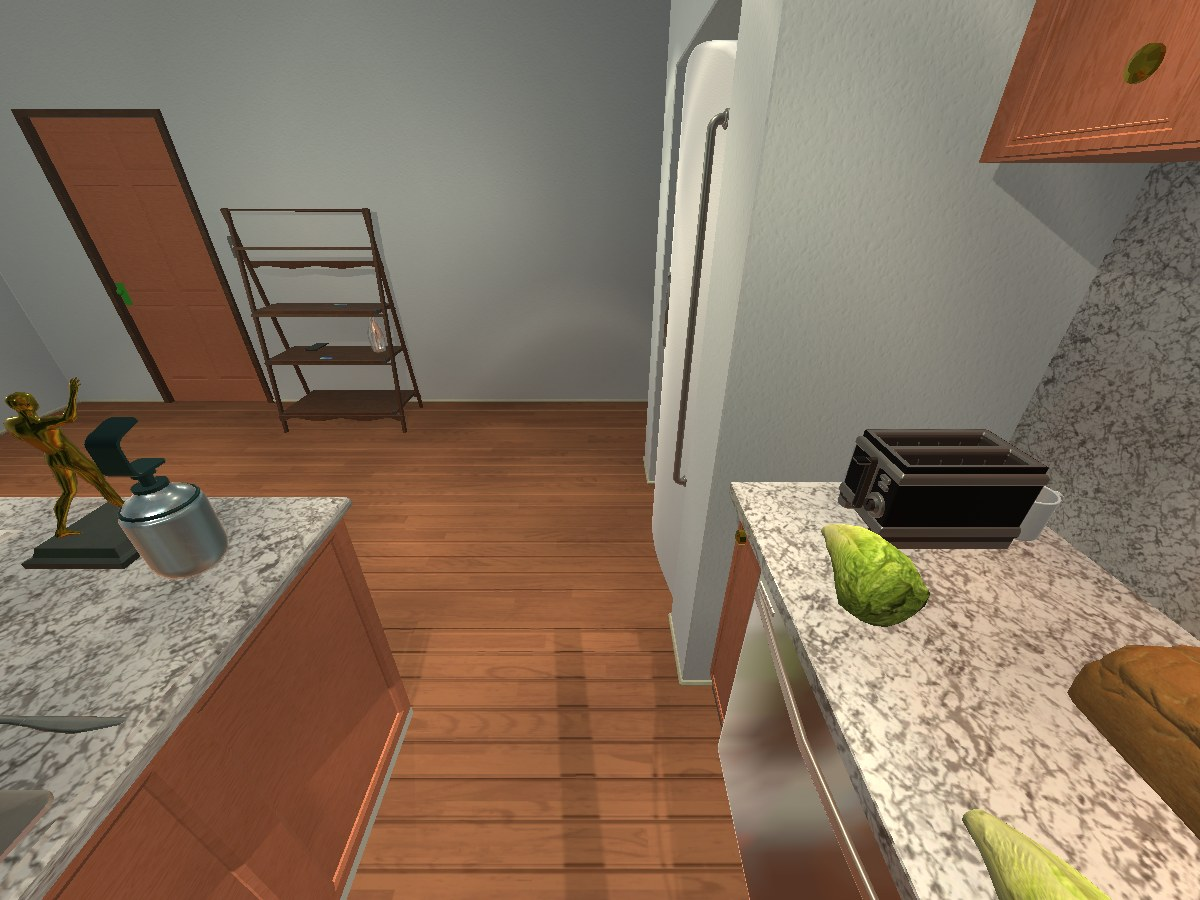
\includegraphics[width=8.815cm]{figures/cases/cool_view1.jpg}};
\draw[black!35, line width=0.4pt] (0.000,0.000) rectangle ++(8.815,-6.611);
\draw[dimF, line width=1.1pt] (7.628,-3.776) circle (0.238);
\draw[lead=dimF] (7.628,-3.776) -- (7.628,-3.276);
\fill[dimF] (7.628,-3.776) circle (0.06);
\node[lblkey=dimF] at (7.628,-3.276) {mug};
\draw[dimA, line width=1.1pt, rounded corners=1pt] (5.377,-3.541) rectangle (8.807,-6.611);
\draw[lead=dimA] (7.092,-5.076) -- (6.653,-4.614);
\fill[dimA] (7.092,-5.076) circle (0.06);
\node[lblkey=dimA] at (6.653,-4.614) {countertop: the mug is here};
\draw[dimE, line width=1.1pt, rounded corners=1pt] (4.789,-0.301) rectangle (5.414,-4.385);
\draw[lead=dimE] (5.102,-2.343) -- (5.102,-1.843);
\fill[dimE] (5.102,-2.343) circle (0.06);
\node[lblkey=dimE] at (5.102,-1.843) {fridge: cool it here};
\draw[liftpositive, line width=1.1pt, rounded corners=1pt] (7.316,-0.007) rectangle (8.807,-1.161);
\draw[lead=liftpositive] (8.062,-0.584) -- (7.068,-0.230);
\fill[liftpositive] (8.062,-0.584) circle (0.06);
\node[lblkey=liftpositive] at (7.068,-0.230) {cabinet: put it here};
\fill[black!55] (1.216,-5.079) circle (0.06);
\node[lbl=black!45] at (1.216,-5.079) {countertop};
\draw[lead=black!55] (6.931,-3.596) -- (6.664,-3.134);
\fill[black!55] (6.931,-3.596) circle (0.06);
\node[lbl=black!45] at (6.664,-3.134) {toaster};
\draw[lead=black!55] (5.399,-4.587) -- (5.399,-4.087);
\fill[black!55] (5.399,-4.587) circle (0.06);
\node[lbl=black!45] at (5.399,-4.087) {cabinet};
\node[anchor=north west, inner sep=0] at (9.065,0.000) {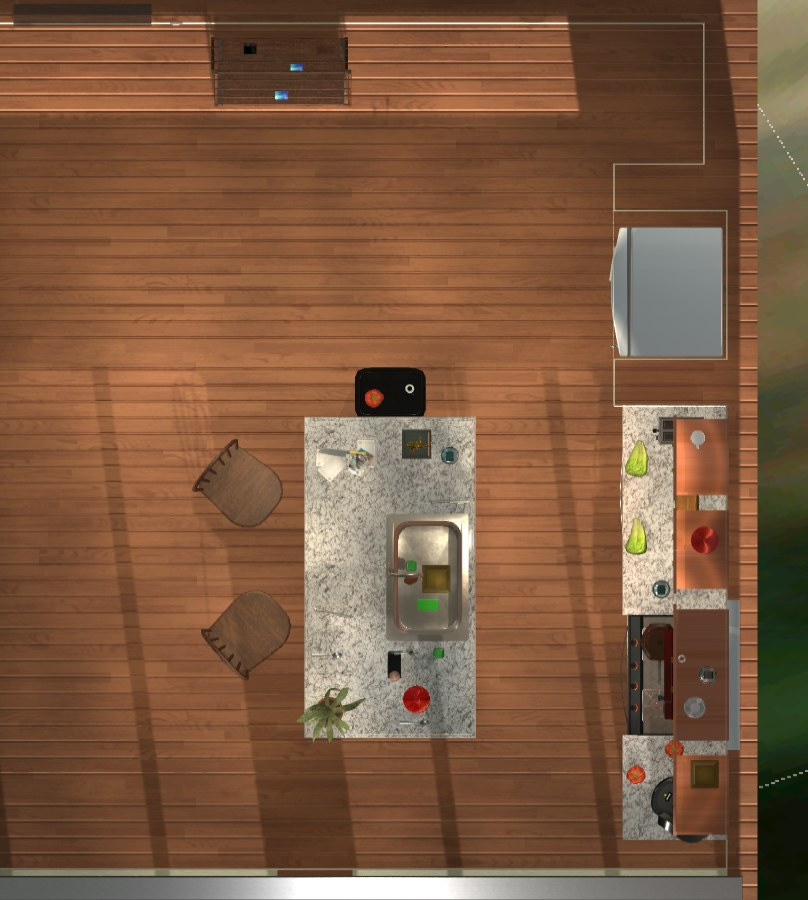
\includegraphics[width=5.935cm]{figures/cases/cool_map.jpg}};
\draw[black!35, line width=0.4pt] (9.065,0.000) rectangle ++(5.935,-6.611);
\fill[black, opacity=0.22] (13.252,-4.077) -- ++(45:1.1) arc (45:135:1.1) -- cycle;
\fill[black] (13.252,-4.077) circle (0.08);
\draw[white, line width=3.4pt, opacity=0.85] (14.008,-3.555) -- (14.035,-2.394);
\draw[path] (14.008,-3.555) -- (14.035,-2.394);
\draw[white, line width=3.4pt, opacity=0.85] (14.038,-2.344) -- (14.025,-3.430);
\draw[path] (14.038,-2.344) -- (14.025,-3.430);
\draw[lead=dimA] (14.003,-3.755) -- (12.803,-3.402);
\fill[dimA] (14.003,-3.755) circle (0.06);
\node[lblkey=dimA] at (12.803,-3.402) {countertop: the mug is here};
\draw[lead=dimE] (14.041,-2.144) -- (13.662,-1.682);
\fill[dimE] (14.041,-2.144) circle (0.06);
\node[lblkey=dimE] at (13.662,-1.682) {fridge: cool it here};
\draw[lead=liftpositive] (14.022,-3.680) -- (13.528,-2.941);
\fill[liftpositive] (14.022,-3.680) circle (0.06);
\node[lblkey=liftpositive] at (13.528,-2.941) {cabinet: put it here};
\draw[lead=black!55] (13.857,-3.809) -- (14.132,-4.271);
\fill[black!55] (13.857,-3.809) circle (0.06);
\node[lbl=black!45] at (14.132,-4.271) {cabinets};
\draw[lead=black!55] (13.912,-5.682) -- (13.912,-5.182);
\fill[black!55] (13.912,-5.682) circle (0.06);
\node[lbl=black!45] at (13.912,-5.182) {cabinets};
\draw[lead=black!55] (14.098,-5.925) -- (12.896,-5.734);
\fill[black!55] (14.098,-5.925) circle (0.06);
\node[lbl=black!45] at (12.896,-5.734) {coffeemachine};
\draw[lead=black!55] (11.611,-4.235) -- (10.913,-3.881);
\fill[black!55] (11.611,-4.235) circle (0.06);
\node[lbl=black!45] at (10.913,-3.881) {countertop};
\draw[lead=black!55] (14.003,-5.786) -- (13.305,-6.140);
\fill[black!55] (14.003,-5.786) circle (0.06);
\node[lbl=black!45] at (13.305,-6.140) {countertop};
\draw[lead=black!55] (13.679,-4.242) -- (12.779,-4.433);
\fill[black!55] (13.679,-4.242) circle (0.06);
\node[lbl=black!45] at (12.779,-4.433) {drawers};
\draw[lead=black!55] (11.933,-2.891) -- (11.933,-2.391);
\fill[black!55] (11.933,-2.891) circle (0.06);
\node[lbl=black!45] at (11.933,-2.391) {garbagecan};
\draw[lead=black!55] (14.125,-4.954) -- (14.125,-3.854);
\fill[black!55] (14.125,-4.954) circle (0.06);
\node[lbl=black!45] at (14.125,-3.854) {microwave};
\draw[lead=black!55] (11.115,-0.530) -- (10.215,-0.339);
\fill[black!55] (11.115,-0.530) circle (0.06);
\node[lbl=black!45] at (10.215,-0.339) {shelves};
\draw[lead=black!55] (12.207,-4.239) -- (11.207,-4.430);
\fill[black!55] (12.207,-4.239) circle (0.06);
\node[lbl=black!45] at (11.207,-4.430) {sinkbasin};
\draw[lead=black!55] (14.034,-4.960) -- (12.426,-4.960);
\fill[black!55] (14.034,-4.960) circle (0.06);
\node[lbl=black!45] at (12.426,-4.960) {stoveburners};
\draw[lead=black!55] (14.060,-3.164) -- (14.060,-2.364);
\fill[black!55] (14.060,-3.164) circle (0.06);
\node[lbl=black!45] at (14.060,-2.364) {toaster};
\node[imgcap] at (4.407,-6.651) {first-person view inside the room};
\node[imgcap] at (12.032,-6.651) {the room from above; cone: the left view; arrow: the expert's route};
\node[anchor=west, font=\sffamily\bfseries\footnotesize, text=black!70] at (0,-7.411) {Expert solution (6 steps):};
\node[chip, anchor=west] (s0) at (3.900,-7.411) {go to countertop};
\node[chip, anchor=west] (s1) at (6.872,-7.411) {take mug from countertop};
\draw[flow] (s0.east) -- (s1.west);
\node[chip, anchor=west] (s2) at (10.980,-7.411) {go to fridge};
\draw[flow] (s1.east) -- (s2.west);
\node[chip, anchor=west] (s3) at (3.900,-7.911) {cool mug with fridge};
\node[chip, anchor=west] (s4) at (7.440,-7.911) {go to cabinet};
\draw[flow] (s3.east) -- (s4.west);
\node[chip, anchor=west] (s5) at (9.986,-7.911) {move mug to cabinet};
\draw[flow] (s4.east) -- (s5.west);
\node[ptitle] at (0.000,-8.711) {(b) Effect of the memory on this family, 3 demonstration pairs};
\node[txt, text=black!65] at (0.000,-9.161) {family success: GPT $0.857\rightarrow0.746$, Qwen $0.857\rightarrow0.857$};
\draw[black!45] (7.400,-9.561) -- (7.400,-12.351);
\node[font=\sffamily\scriptsize, text=black!50] at (5.000,-12.521) {$-1$};
\node[font=\sffamily\scriptsize, text=black!50] at (7.400,-12.521) {$0$};
\node[font=\sffamily\scriptsize, text=black!50] at (9.800,-12.521) {$+1$};
\node[lab] at (4.850,-9.831) {task 5};
\fill[gptblue!55] (7.400,-9.681) rectangle ++(-1.200,-0.24);
\node[anchor=east, font=\sffamily\scriptsize, text=black!70] at (6.140,-9.801) {$-0.500$};
\fill[qwenmint!55] (7.400,-9.971) rectangle ++(-0.799,-0.24);
\node[anchor=east, font=\sffamily\scriptsize, text=black!70] at (6.541,-10.091) {$-0.333$};
\node[lab] at (4.850,-10.491) {task 16};
\fill[gptblue!55] (7.400,-10.341) rectangle ++(-0.799,-0.24);
\node[anchor=east, font=\sffamily\scriptsize, text=black!70] at (6.541,-10.461) {$-0.333$};
\fill[qwenmint!55] (7.400,-10.631) rectangle ++(0.000,-0.24);
\node[anchor=west, font=\sffamily\scriptsize, text=black!70] at (7.460,-10.751) {$0$};
\node[lab] at (4.850,-11.151) {task 19};
\fill[gptblue!55] (7.400,-11.001) rectangle ++(-0.799,-0.24);
\node[anchor=east, font=\sffamily\scriptsize, text=black!70] at (6.541,-11.121) {$-0.333$};
\fill[qwenmint!55] (7.400,-11.291) rectangle ++(0.000,-0.24);
\node[anchor=west, font=\sffamily\scriptsize, text=black!70] at (7.460,-11.411) {$0$};
\node[lab] at (4.850,-11.811) {task 39};
\fill[gptblue!55] (7.400,-11.661) rectangle ++(0.000,-0.24);
\node[anchor=west, font=\sffamily\scriptsize, text=black!70] at (7.460,-11.781) {$0$};
\fill[qwenmint!55] (7.400,-11.951) rectangle ++(0.799,-0.24);
\node[anchor=west, font=\sffamily\scriptsize, text=black!70] at (8.259,-12.071) {$+0.333$};
\fill[gptblue!55] (0.000,-9.911) rectangle ++(0.28,-0.18);
\node[txt] at (0.320,-10.001) {GPT-4o-mini};
\fill[qwenmint!55] (0.000,-10.311) rectangle ++(0.28,-0.18);
\node[txt] at (0.320,-10.401) {Qwen3-8B};
\end{scope}
\end{tikzpicture}
}
\end{center}
\vspace{-4pt}
\captionof{figure}{The \texttt{cool} family. (a) An example \texttt{cool} task, in the kitchen: the mug starts on a countertop, must be cooled in the fridge, and goes into a cabinet. (b) Memory effect on four representative tasks.}
\label{fig:case_cool}
\vspace{4pt}

\textbf{The tasks.} The agent must cool an object in the fridge and place it somewhere,
typically in a kitchen. Frequent objects are mugs, lettuce, pans, bread, and potatoes;
frequent destinations are countertops and the microwave.

\textbf{What it takes.} Six steps on average (4--7): find the object, take it,
\texttt{go to fridge}, \texttt{cool <object> with fridge}, go to the destination, and
place it.

\textbf{What the memory offers.} Six \texttt{[cool]} rules (items 5--10), such as ``Always
check the fridge first for items that need to be cooled'' and ``Maintain a clear sequence
of actions: find, cool, and place the item''. The first \texttt{[cool]} rule is ranked 2nd
for task 5.

\textbf{What happened.} Family: \gptm $0.857\rightarrow0.746$, the only family in which
\gptm loses; \qwenm $0.857\rightarrow0.857$. Task 5: \gptm $-0.500$ and \qwenm $-0.333$,
with \qwenm solving it on every pair without memory; it is one of the six tasks harmed
under both stacks. Other \texttt{cool} tasks: tasks 16 and 19 (\gptm $-0.333$, \qwenm
$0.000$) and task 39 (\gptm $0.000$, \qwenm $+0.333$).

\textbf{Analysis.} \texttt{cool} is \gptm's strongest family without memory, and it is
where the memory hurts \gptm. The rules restate a procedure both executors already
follow, and one of them (``Always check the fridge first'') points the search at the
fridge, where the object must be cooled but is not necessarily found; the retained data
cannot show whether this redirected the search. Harm concentrates where the no-memory
harness is already strong, for either executor.
\end{casebox}

\begin{casebox}[dimE]{Case 6 \textperiodcentered{} \texttt{examine} \textperiodcentered{} family of 18 tasks; representative task 7}
\begin{center}
\resizebox{\linewidth}{!}{\begin{tikzpicture}[x=1cm, y=1cm, font=\sffamily\footnotesize,
  ptitle/.style={anchor=west, font=\sffamily\bfseries\small, text=narrareddeep},
  textbox/.style={draw=phaseA!60, fill=phaseA!6, rounded corners=2pt, inner sep=4pt, anchor=north west,
                  align=left, font=\sffamily\scriptsize},
  lbl/.style={draw=#1, fill=white, fill opacity=0.9, text opacity=1, rounded corners=1pt, inner sep=1.6pt,
              line width=0.6pt, font=\sffamily\scriptsize},
  lblkey/.style={draw=#1, fill=white, fill opacity=0.95, text opacity=1, rounded corners=1pt, inner sep=1.8pt,
                 line width=1.0pt, font=\sffamily\scriptsize\bfseries},
  lead/.style={draw=#1, line width=0.7pt},
  path/.style={-{Latex[length=2.6mm, width=2.4mm]}, draw=black!85, line width=1.6pt},
  imgcap/.style={anchor=north, font=\sffamily\scriptsize, text=black!60},
  chip/.style={draw=black!30, fill=white, rounded corners=6pt, inner sep=2.5pt, font=\sffamily\footnotesize},
  flow/.style={-{Latex[length=1.6mm]}, draw=black!50, line width=0.6pt},
  lab/.style={anchor=east, font=\sffamily\footnotesize, text=black!75},
  txt/.style={anchor=west, font=\sffamily\footnotesize, text=black!75}]

\node[ptitle] at (0,0.000) {(a) An example task of this family and its room (AI2-THOR rendering)};
\node[textbox, text width=14.70cm] (obs) at (0,-0.280) {\textbf{Goal.} Your task is to: examine the book with the desklamp.\\[1pt]\textbf{Initial observation.} You are in the middle of a room. Looking quickly around you, you see a bed 1, a desk 2, a desk 1, a drawer 6, a drawer 5, a drawer 4, a drawer 3, a drawer 2, a drawer 1, a garbagecan 1, a laundryhamper 1, a safe 1, a shelf 6, a shelf 5, a shelf 4, a shelf 3, a shelf 2, and a shelf 1.};
\begin{scope}[shift={($(obs.south west)+(0,-0.25)$)}]
\node[anchor=north west, inner sep=0] at (0.000,0.000) {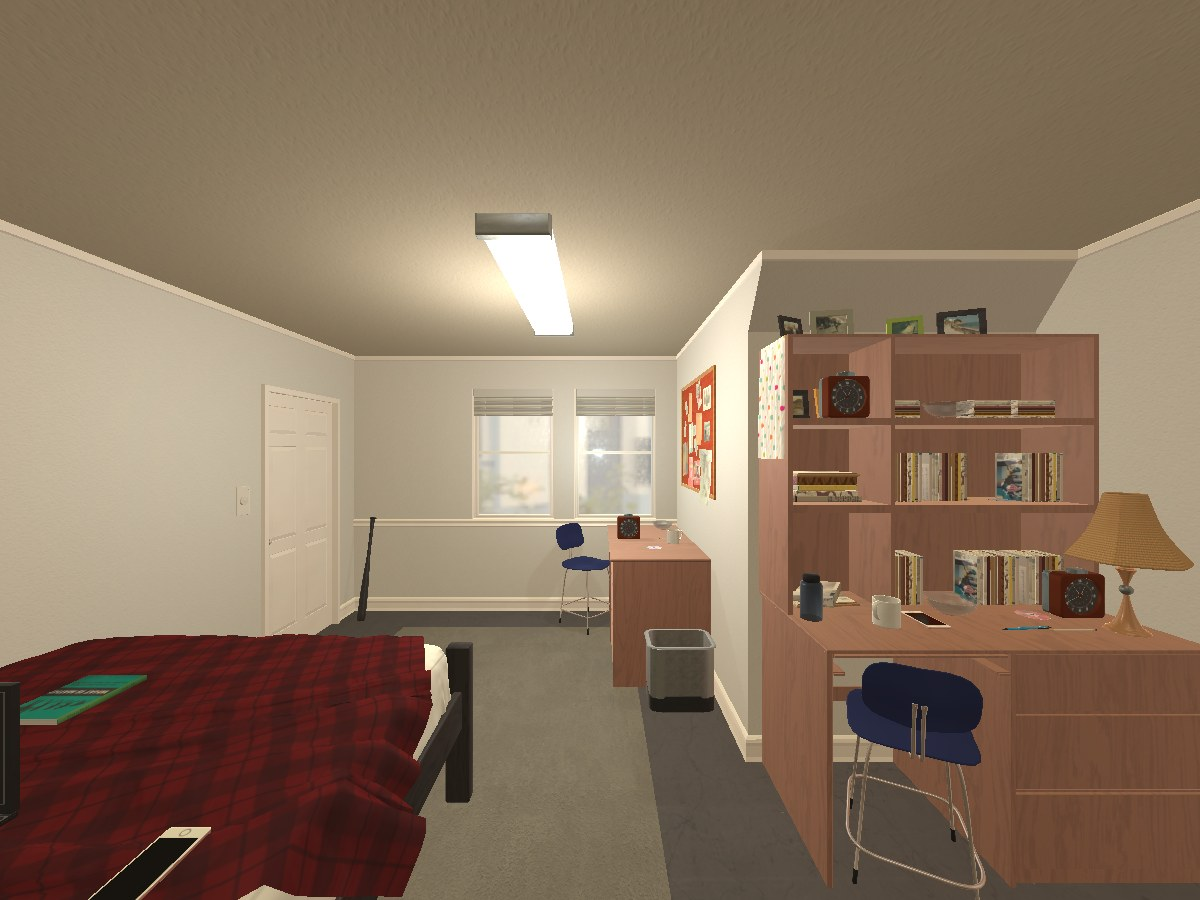
\includegraphics[width=8.487cm]{figures/cases/examine_view1.jpg}};
\draw[black!35, line width=0.4pt] (0.000,0.000) rectangle ++(8.487,-6.365);
\draw[dimF, line width=1.1pt] (0.587,-4.954) circle (0.535);
\draw[lead=dimF] (0.587,-4.954) -- (0.587,-4.454);
\fill[dimF] (0.587,-4.954) circle (0.06);
\node[lblkey=dimF] at (0.587,-4.454) {book};
\draw[dimA, line width=1.1pt, rounded corners=1pt] (0.000,-4.491) rectangle (3.338,-6.365);
\fill[dimA] (1.669,-5.428) circle (0.06);
\node[lblkey=dimA] at (1.669,-5.428) {bed: the book is here};
\draw[dimE, line width=1.1pt, rounded corners=1pt] (7.525,-3.487) rectangle (8.438,-4.512);
\draw[lead=dimE] (7.981,-4.000) -- (6.988,-3.646);
\fill[dimE] (7.981,-4.000) circle (0.06);
\node[lblkey=dimE] at (6.988,-3.646) {desklamp: turn it on};
\fill[black!55] (6.928,-5.234) circle (0.06);
\node[lbl=black!45] at (6.928,-5.234) {desks};
\draw[lead=black!55] (7.030,-3.989) -- (6.130,-4.180);
\fill[black!55] (7.030,-3.989) circle (0.06);
\node[lbl=black!45] at (6.130,-4.180) {shelves};
\draw[lead=black!55] (7.833,-5.877) -- (6.933,-5.686);
\fill[black!55] (7.833,-5.877) circle (0.06);
\node[lbl=black!45] at (6.933,-5.686) {drawers};
\node[anchor=north west, inner sep=0] at (8.737,0.000) {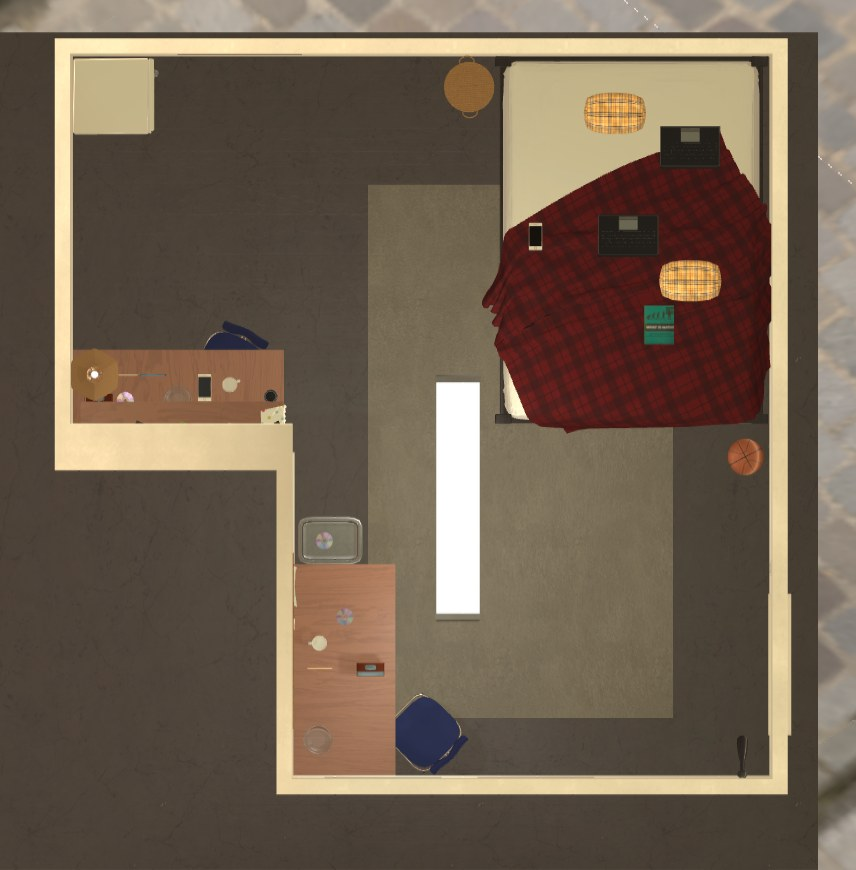
\includegraphics[width=6.263cm]{figures/cases/examine_map.jpg}};
\draw[black!35, line width=0.4pt] (8.737,0.000) rectangle ++(6.263,-6.365);
\fill[black, opacity=0.22] (11.708,-0.789) -- ++(-135:1.1) arc (-135:-45:1.1) -- cycle;
\fill[black] (11.708,-0.789) circle (0.08);
\draw[white, line width=3.4pt, opacity=0.85] (13.163,-1.765) -- (9.665,-2.678);
\draw[path] (13.163,-1.765) -- (9.665,-2.678);
\draw[lead=dimA] (13.357,-1.715) -- (13.357,-1.215);
\fill[dimA] (13.357,-1.715) circle (0.06);
\node[lblkey=dimA] at (13.357,-1.215) {bed: the book is here};
\draw[lead=dimE] (9.423,-2.741) -- (10.416,-3.094);
\fill[dimE] (9.423,-2.741) circle (0.06);
\node[lblkey=dimE] at (10.416,-3.094) {desklamp: turn it on};
\draw[lead=black!55] (10.223,-2.835) -- (10.223,-2.335);
\fill[black!55] (10.223,-2.835) circle (0.06);
\node[lbl=black!45] at (10.223,-2.335) {desk};
\draw[lead=black!55] (11.356,-5.082) -- (11.356,-4.582);
\fill[black!55] (11.356,-5.082) circle (0.06);
\node[lbl=black!45] at (11.356,-4.582) {desk};
\draw[lead=black!55] (9.672,-2.767) -- (9.291,-2.028);
\fill[black!55] (9.672,-2.767) circle (0.06);
\node[lbl=black!45] at (9.291,-2.028) {drawers};
\draw[lead=black!55] (11.424,-4.531) -- (11.424,-4.031);
\fill[black!55] (11.424,-4.531) circle (0.06);
\node[lbl=black!45] at (11.424,-4.031) {drawers};
\draw[lead=black!55] (11.153,-3.956) -- (10.454,-3.602);
\fill[black!55] (11.153,-3.956) circle (0.06);
\node[lbl=black!45] at (10.454,-3.602) {garbagecan};
\draw[lead=black!55] (12.169,-0.637) -- (11.382,-0.283);
\fill[black!55] (12.169,-0.637) circle (0.06);
\node[lbl=black!45] at (11.382,-0.283) {laundryhamper};
\draw[lead=black!55] (9.550,-0.704) -- (9.309,-0.242);
\fill[black!55] (9.550,-0.704) circle (0.06);
\node[lbl=black!45] at (9.309,-0.242) {safe};
\draw[lead=black!55] (10.174,-3.124) -- (9.678,-4.140);
\fill[black!55] (10.174,-3.124) circle (0.06);
\node[lbl=black!45] at (9.678,-4.140) {shelves};
\node[imgcap] at (4.244,-6.405) {first-person view inside the room};
\node[imgcap] at (11.869,-6.405) {the room from above; cone: the left view; arrow: the expert's route};
\node[anchor=west, font=\sffamily\bfseries\footnotesize, text=black!70] at (0,-7.165) {Expert solution (4 steps):};
\node[chip, anchor=west] (s0) at (3.900,-7.165) {go to bed};
\node[chip, anchor=west] (s1) at (5.878,-7.165) {take book from bed};
\draw[flow] (s0.east) -- (s1.west);
\node[chip, anchor=west] (s2) at (9.134,-7.165) {go to desk};
\draw[flow] (s1.east) -- (s2.west);
\node[chip, anchor=west] (s3) at (11.254,-7.165) {use desklamp};
\draw[flow] (s2.east) -- (s3.west);
\node[ptitle] at (0.000,-7.965) {(b) Effect of the memory on this family, 3 demonstration pairs};
\node[txt, text=black!65] at (0.000,-8.415) {family success: GPT $0.648\rightarrow0.833$, Qwen $0.611\rightarrow0.574$};
\draw[black!45] (7.400,-8.815) -- (7.400,-10.945);
\node[font=\sffamily\scriptsize, text=black!50] at (5.000,-11.115) {$-1$};
\node[font=\sffamily\scriptsize, text=black!50] at (7.400,-11.115) {$0$};
\node[font=\sffamily\scriptsize, text=black!50] at (9.800,-11.115) {$+1$};
\node[lab] at (4.850,-9.085) {task 7};
\fill[gptblue!55] (7.400,-8.935) rectangle ++(1.601,-0.24);
\node[anchor=west, font=\sffamily\scriptsize, text=black!70] at (9.061,-9.055) {$+0.667$};
\fill[qwenmint!55] (7.400,-9.225) rectangle ++(0.799,-0.24);
\node[anchor=west, font=\sffamily\scriptsize, text=black!70] at (8.259,-9.345) {$+0.333$};
\node[lab] at (4.850,-9.745) {task 45};
\fill[gptblue!55] (7.400,-9.595) rectangle ++(1.601,-0.24);
\node[anchor=west, font=\sffamily\scriptsize, text=black!70] at (9.061,-9.715) {$+0.667$};
\fill[qwenmint!55] (7.400,-9.885) rectangle ++(-1.601,-0.24);
\node[anchor=east, font=\sffamily\scriptsize, text=black!70] at (5.739,-10.005) {$-0.667$};
\node[lab] at (4.850,-10.405) {task 89};
\fill[gptblue!55] (7.400,-10.255) rectangle ++(-1.200,-0.24);
\node[anchor=east, font=\sffamily\scriptsize, text=black!70] at (6.140,-10.375) {$-0.500$};
\fill[qwenmint!55] (7.400,-10.545) rectangle ++(0.000,-0.24);
\node[anchor=west, font=\sffamily\scriptsize, text=black!70] at (7.460,-10.665) {$0$};
\fill[gptblue!55] (0.000,-9.165) rectangle ++(0.28,-0.18);
\node[txt] at (0.320,-9.255) {GPT-4o-mini};
\fill[qwenmint!55] (0.000,-9.565) rectangle ++(0.28,-0.18);
\node[txt] at (0.320,-9.655) {Qwen3-8B};
\end{scope}
\end{tikzpicture}
}
\end{center}
\vspace{-4pt}
\captionof{figure}{The \texttt{examine} family. (a) An example \texttt{examine} task, in the bedroom: the book lies on the bed, and the agent must carry it to the desk and turn on the desk lamp while holding it. (b) Memory effect on three representative tasks.}
\label{fig:case_examine}
\vspace{4pt}

\textbf{The tasks.} The agent must look at an object under a desk lamp, in bedrooms. Frequent objects are mugs, pencils, bowls, CDs, and books.

\textbf{What it takes.} The shortest family, 3.8 steps on average (3--4): find the object,
take it, \texttt{go to} the desk lamp, and \texttt{use desklamp}. The difficulty is
finding the object and recognizing that ``examine'' means turning on the lamp while
holding it.

\textbf{What the memory offers.} Six \texttt{[examine]} rules (items 11--16), including
``Use the most probable locations for the second required item after obtaining the
first'' and ``Ensure to use the item in the correct context to achieve the task's goal''.
For task 7 the first \texttt{[examine]} rule is ranked only 7th.

\textbf{What happened.} Family: \gptm $0.648\rightarrow0.833$, \qwenm
$0.611\rightarrow0.574$. Task 7: \gptm $+0.667$ and \qwenm $+0.333$ from a \qwenm
no-memory success of $0.333$, one of only nine tasks that improve under both stacks.
Task 45, of the same family, shows the reversal instead (\gptm $+0.667$, \qwenm
$-0.667$, from a \qwenm no-memory success of $0.667$), and task 89 harms \gptm
($-0.500$).

\textbf{Analysis.} Joint improvement happens on a task where both executors start low,
even though the matching rule is far down the block. With a higher \qwenm baseline, the
same family produces the reversal. Baseline competence, not rule position, best
separates the two outcomes in these cases.
\end{casebox}

\begin{casebox}[salmon]{Case 7 \textperiodcentered{} WebShop \textperiodcentered{} 100 train-disjoint sessions}
\begin{center}
\resizebox{\linewidth}{!}{\begin{tikzpicture}[x=1cm, y=1cm, font=\sffamily\footnotesize,
  ptitle/.style={anchor=west, font=\sffamily\bfseries\small, text=narrareddeep},
  textbox/.style={draw=phaseA!60, fill=phaseA!6, rounded corners=2pt, inner sep=4pt, anchor=north west,
                  align=left, font=\sffamily\scriptsize},
  lbl/.style={draw=#1, fill=white, fill opacity=0.9, text opacity=1, rounded corners=1pt, inner sep=1.6pt,
              line width=0.6pt, font=\sffamily\scriptsize},
  lblkey/.style={draw=#1, fill=white, fill opacity=0.95, text opacity=1, rounded corners=1pt, inner sep=1.8pt,
                 line width=1.0pt, font=\sffamily\scriptsize\bfseries},
  lead/.style={draw=#1, line width=0.7pt},
  path/.style={-{Latex[length=2.6mm, width=2.4mm]}, draw=black!85, line width=1.6pt},
  imgcap/.style={anchor=north, font=\sffamily\scriptsize, text=black!60},
  chip/.style={draw=black!30, fill=white, rounded corners=6pt, inner sep=2.5pt, font=\sffamily\footnotesize},
  flow/.style={-{Latex[length=1.6mm]}, draw=black!50, line width=0.6pt},
  lab/.style={anchor=east, font=\sffamily\footnotesize, text=black!75},
  txt/.style={anchor=west, font=\sffamily\footnotesize, text=black!75}]

\node[ptitle] at (0,0) {(a) One WebShop session in the official web app (evaluation session 0)};
\node[anchor=south west, align=left, text width=5.40cm, font=\sffamily\scriptsize, text=black!75, inner sep=1pt] at (0.000,-1.650) {The start page shows the request and a search box.};
\node[anchor=north west, inner sep=0] at (0.000,-1.750) {
\includegraphics[width=5.500cm]{figures/cases/ws_search.jpg}};
\draw[black!35, line width=0.4pt] (0.000,-1.750) rectangle ++(5.500,-2.173);
\node[anchor=south west, align=left, text width=3.85cm, font=\sffamily\scriptsize, text=black!75, inner sep=1pt] at (5.800,-1.650) {After \texttt{search[double sided machine washable decorative pillows 28 x 28]}: 50 results, 10 per page.};
\node[anchor=north west, inner sep=0] at (5.800,-1.750) {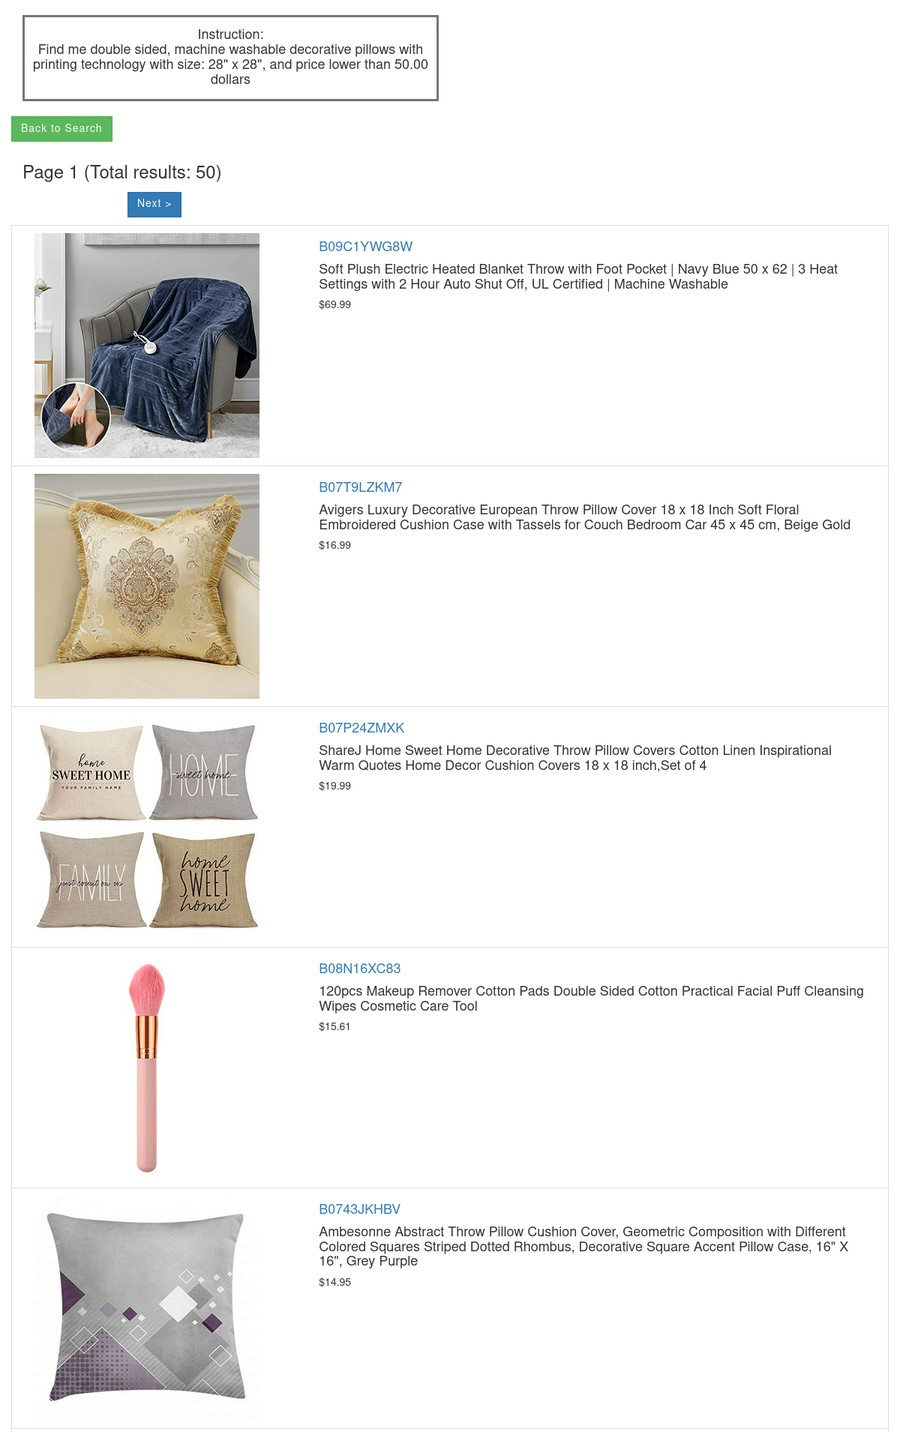
\includegraphics[width=3.950cm]{figures/cases/ws_results.jpg}};
\draw[black!35, line width=0.4pt] (5.800,-1.750) rectangle ++(3.950,-6.285);
\node[anchor=south west, align=left, text width=4.85cm, font=\sffamily\scriptsize, text=black!75, inner sep=1pt] at (10.050,-1.650) {After \texttt{click[B0743JKHBV]}: the product page, with its size options and a \textit{Buy Now} button.};
\node[anchor=north west, inner sep=0] at (10.050,-1.750) {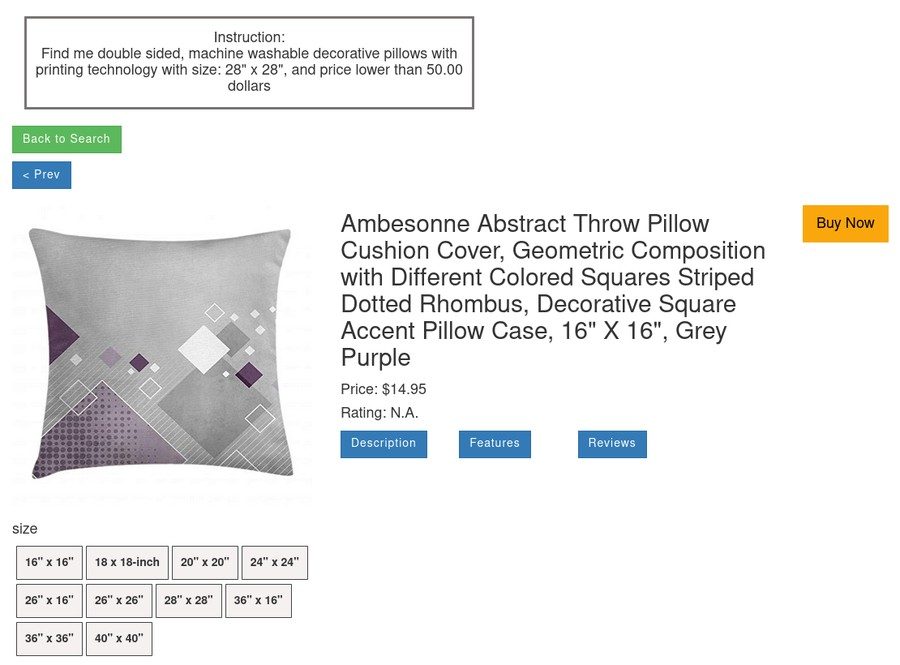
\includegraphics[width=4.950cm]{figures/cases/ws_product.jpg}};
\draw[black!35, line width=0.4pt] (10.050,-1.750) rectangle ++(4.950,-3.658);
\node[anchor=south west, align=left, text width=4.85cm, font=\sffamily\scriptsize, text=black!75, inner sep=1pt] at (10.050,-6.528) {After \texttt{click[28\textquotedbl{} x 28\textquotedbl{}]} and \texttt{click[Buy Now]}: the episode ends; the score box (green) shows reward 1.0.};
\node[anchor=north west, inner sep=0] at (10.050,-6.608) {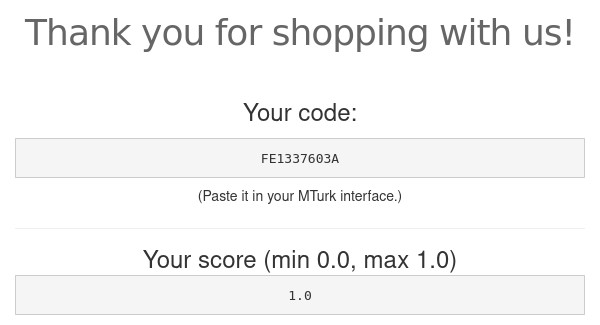
\includegraphics[width=4.950cm]{figures/cases/ws_score.jpg}};
\draw[black!35, line width=0.4pt] (10.050,-6.608) rectangle ++(4.950,-2.681);
\draw[liftpositive, line width=1.2pt, rounded corners=1pt] (5.835,-6.960) rectangle (9.715,-8.026);
\node[lblkey=liftpositive, anchor=center] (hl) at (7.775,-8.355) {the requested product (5th)};
\draw[lead=liftpositive] (hl) -- (7.775,-8.026);
\draw[dimA, line width=1.2pt, rounded corners=1pt] (10.902,-4.957) rectangle (11.277,-5.155);
\node[lblkey=dimA, anchor=west] (hl) at (11.700,-5.056) {\texttt{click[28\textquotedbl{} x 28\textquotedbl{}]}};
\draw[lead=dimA] (hl) -- (11.277,-5.056);
\draw[dimF, line width=1.2pt, rounded corners=1pt] (14.461,-2.872) rectangle (14.940,-3.087);
\node[lblkey=dimF, anchor=east] (hl) at (14.340,-2.674) {\texttt{click[Buy Now]}};
\draw[lead=dimF] (hl) -- (14.461,-2.872);
\draw[liftpositive, line width=1.2pt, rounded corners=1pt] (10.166,-8.868) rectangle (14.885,-9.215);
\node[textbox, text width=5.20cm] at (0.000,-4.223) {\textbf{What the reward checks.} The purchase is compared with the request:\\[1pt]\textbullet\ attributes: double sided, machine washable, printing technology\\\textbullet\ option: size 28\textquotedbl{} x 28\textquotedbl{}\\\textbullet\ price: lower than \$50.00\\\textbullet\ product type: the title must match the request\\[2pt]The reward is the share of matched attributes, options, and price, times the type match; here everything matches, so it is 1.0. A session allows at most 15 actions, and the store holds 1{,}000 products. The ranking shown comes from our BM25 stand-in for the search index.};
\draw[flow, line width=1pt] (5.530,-2.850) -- (5.770,-2.850);
\draw[flow, line width=1pt] (9.780,-2.850) -- (10.020,-2.850);
\draw[flow, line width=1pt] (9.930,-5.108) |- (10.020,-7.108);
\node[ptitle] at (0,-10.039) {(b) What happened: \texttt{Qwen3-8B}, 100 sessions};
\node[lab] at (1.650,-10.639) {no memory};
\fill[phaseA!35, rounded corners=1pt] (1.750,-10.489) rectangle ++(4.666,-0.3);
\node[txt] at (6.496,-10.639) {mean reward 0.194};
\node[lab] at (1.650,-11.099) {memory};
\fill[salmon!60, rounded corners=1pt] (1.750,-10.949) rectangle ++(2.508,-0.3);
\node[txt] at (4.338,-11.099) {mean reward 0.105};
\node[txt] at (9.600,-10.639) {paired change per session:};
\fill[salmon!60] (9.600,-10.939) rectangle ++(1.080,-0.36);
\node[font=\sffamily\footnotesize] at (10.140,-11.119) {20};
\node[font=\sffamily\scriptsize, text=black!65, anchor=north] at (10.140,-11.339) {declined};
\fill[black!12] (10.680,-10.939) rectangle ++(3.888,-0.36);
\node[font=\sffamily\footnotesize] at (12.624,-11.119) {72};
\node[font=\sffamily\scriptsize, text=black!65, anchor=north] at (12.624,-11.339) {unchanged};
\fill[qwenmint!55] (14.568,-10.939) rectangle ++(0.432,-0.36);
\node[font=\sffamily\footnotesize] at (14.784,-11.119) {8};
\node[font=\sffamily\scriptsize, text=black!65, anchor=north] at (14.784,-11.339) {improved};
\end{tikzpicture}
}
\end{center}
\vspace{-4pt}
\captionof{figure}{WebShop. (a) One session in the official web app: the start page with the request, the results of a search, the product page where the size is chosen, and the score page after the purchase. The query and clicks are ours; the reward of 1.0 shows what a full match looks like. (b) Mean reward and the sign of the paired reward change over 100 sessions.}
\label{fig:case_webshop}
\vspace{4pt}

\textbf{The tasks.} Each WebShop session gives a natural-language request for a product
with required attributes, options, and a price limit, in a simulated store of 1{,}000
products. The agent searches, opens product pages, selects options, and buys; the
environment reward measures how well the purchased product matches the request, and
exact success requires a full match. Episodes are limited to 15 steps.

\textbf{What the memory offers.} Ten rules about search, attribute checking, option
selection, and purchase, distilled by \qwenm with the prompt of
Appendix~\ref{app:prompts} from the six positive-reward trajectories of train sessions
500--519, and presented by BM25 with $B=1{,}024$.

\textbf{What happened.} A 20-session gate confirmed valid execution (100\% valid action
syntax, search on 20/20, 13 purchase attempts, mean reward $0.288$). On sessions 0--99,
reward falls from $0.194$ to $0.105$ (paired $-0.090$, \ci{-0.165}{-0.016}) and exact
success from $0.09$ to $0.07$; 8 sessions improve, 20 decline, and 72 are unchanged.

\textbf{Analysis.} The experience behind the memory is thin, six successful
trajectories, and the executor reading it is the one that showed no ALFWorld gain. The
rules lower reward on twice as many sessions as they raise it. This case has one
executor and no placebo, so it shows negative transfer but cannot separate content from
context.
\end{casebox}

\section{Seed-Axis Audit}
\label{app:seedaxis}

The scaffold selects two of three demonstrations per task type with a seeded
shuffle. Nominal seeds 0, 1, and 2 map to pairs 02, 12, and 12, so seeds 1 and 2
repeat one prompt condition and pair 01 was missing from the original matrix. Seeds
1 and 2 disagree on 20.9\% of \gptm no-memory task outcomes but on only 1.5\% of
\qwenm outcomes despite identical prompts, which reflects residual hosted
nondeterminism. Weighting the two observed pairs equally gives a \gptm gain of
$+0.134$ (\ci{+0.069}{+0.200}), a \qwenm change of $-0.035$ (\ci{-0.082}{+0.011}),
and a gap of $-0.170$ (\ci{-0.252}{-0.088}). After seed 5 supplied pair 01, the
complete three-pair estimates are those reported in RQ1 and RQ2. Repeated
executions of one prompt are averaged within pair and never treated as independent
seeds.

\section{Order-Placebo Construction}
\label{app:placebo}

The placebo is built in three deterministic steps: (i) shuffle the body words of
each item, re-drawing until no original adjacent body bigram remains; (ii) greedily
replace words with the nonce \texttt{x} until the payload measures exactly 645
tokens under both the \gptm and \qwenm tokenizers (28 of 472 words); (iii) serve the
payload through the ranking-reference path so that BM25 scores are computed on the
original text. The released builder regenerates the placebo exactly (645 tokens
before and 673 after shuffling, 28 substitutions, 94.07\% of body words retained,
645/645 tokens under both tokenizers), and the runtime audit confirmed identical
order on 134/134 queries and all 33 items present. Table~\ref{tab:placebo} shows two
items.

\begin{table}[t]
\centering
\caption{Examples of the order placebo. Task tags, item indices, word counts,
retrieval order, and total footprint are preserved.}
\label{tab:placebo}
\footnotesize
\setlength{\tabcolsep}{6pt}
\renewcommand{\arraystretch}{1.25}
\arrayrulecolor{tableline}
\begin{tabular}{@{}L{0.46\textwidth}L{0.46\textwidth}@{}}
\toprule
\rowcolor{tableheadbg}
\tablehead{True insight} & \tablehead{Index-aligned order placebo} \\
\midrule
\rowcolor{tablestripebg}
\texttt{[clean]} Identify the target item and its cleaning requirements before starting the task.
& \texttt{[clean]} the the item cleaning its starting requirements x and target Identify before \\
\texttt{[clean]} Always clean the item using the designated cleaning area before placing it in the final location.
& \texttt{[clean]} item final area it the Always the before designated clean in x using placing cleaning the \\
\bottomrule
\end{tabular}
\arrayrulecolor{black}
\vspace{-10pt}
\end{table}
